\documentclass[11pt]{article}

% ---------------------------------------------------------------
% From Limit-Order-Book Information to Executable Decisions
% Survey (theoretical / methodological). No new experiments.
% ---------------------------------------------------------------

\usepackage[utf8]{inputenc}
\usepackage[T1]{fontenc}
\usepackage{lmodern}
\usepackage{amsmath,amssymb,amsthm}
\usepackage{booktabs}
\usepackage{graphicx}
\usepackage{array}
\usepackage{tabularx}
\usepackage{longtable}
\usepackage{geometry}
\usepackage[authoryear,round]{natbib}
\usepackage{xurl}
\usepackage{hyperref}
\usepackage{xcolor}
\usepackage{enumitem}
\usepackage{microtype}
\usepackage{cancel}
\usepackage{listings}
\usepackage{tikz}
\usetikzlibrary{arrows.meta,positioning,shapes.geometric,fit,calc}
\usepackage[font=small,labelfont=bf,skip=4pt]{caption}
\usepackage{placeins}
\usepackage[most]{tcolorbox}

\geometry{margin=1in}
\setlength{\emergencystretch}{2em}
\hypersetup{colorlinks=true, linkcolor=blue!50!black, citecolor=blue!50!black,
            urlcolor=blue!50!black}

\lstset{basicstyle=\ttfamily\small, columns=fullflexible, keepspaces=true,
        frame=single, framerule=0.3pt, xleftmargin=1em, xrightmargin=1em,
        breaklines=true}

% Boxes for worked examples and intuition notes
\newtheoremstyle{example}{6pt}{6pt}{\normalfont}{}{\bfseries}{.}{0.5em}{}
\theoremstyle{example}
\newtheorem{example}{Example}[section]
\newtheorem{principle}{Principle}
\newcommand{\illus}{\textsc{(illustrative)}}
% Plain-language reading of an equation, for undergraduate readers
\newcommand{\inwords}[1]{\par\smallskip\noindent\textit{In words:} #1\par\smallskip}

% Four-question model card used at the end of each model in Part II
\newtcolorbox{modelcard}[1]{breakable, enhanced, colback=black!3, colframe=black!45,
  boxrule=0.5pt, arc=1.5pt, left=5pt, right=5pt, top=3pt, bottom=3pt,
  fonttitle=\bfseries\small, title={Model card: #1}, fontupper=\small}
\newcommand{\cardrow}[2]{\par\noindent\textbf{#1.}\enspace #2\par\smallskip}

\newcommand{\E}{\mathbb{E}}
\renewcommand{\P}{\mathbb{P}}
\newcommand{\OFI}{\mathrm{OFI}}
\newcommand{\QI}{\mathrm{QI}}
\newcommand{\Fill}{\mathrm{Fill}}
\newcommand{\lamd}{\textsc{lamd}}
\newcommand{\pov}{\textsc{Shadow-PPOV}}

\title{\textbf{From Limit-Order-Book Information to Executable Decisions:}\\[2pt]
\Large Signals, Queues, Deterministic Simulation, and LLM-Assisted Model Discovery}

\author{%
  Vincent Maciejewski\\
  \small M2 Technologies\\
  \small \texttt{mayeski@gmail.com}
}

\date{Draft --- \today}

\begin{document}
\maketitle

\begin{abstract}
A large literature predicts short-term price moves from the limit order book (LOB): signals such as order-flow
imbalance and the micro-price, queue and first-passage models, Hawkes and neural point processes, and deep networks
from convolutional models to Transformers and pretrained message-level encoders. Most of it stops at the forecast.
Models are scored on how often they guess the direction of the next move, and in an independent re-test of fifteen
published deep models on later Nasdaq data, F1 scores were between 48\% and 61\%, lower than those reported on FI-2010. A trader needs to know something else: whether the
information a model extracts survives the queue, the fill and the latency of a real order, and still makes money.

This survey follows a model from theory to production. It is three surveys in one, in the order the work is done:
order-book models---how each is built, what it predicts and which simple baselines it must beat; simulators---how a
model becomes a trading strategy and is tested against recorded markets with its orders in the real queues; and
hardware---how a tested strategy is deployed fast enough to run. Its thesis is that what matters for trading is the
expected profit of an action given the market state and the order's place in the queue, not the accuracy of the
forecast behind it.

The survey shows a practitioner how to check each step. The first check is whether a reported accuracy is real. In a
re-test of DeepLOB on a year of Apple data, with the same network, the construction of the label alone moved accuracy
from 65.9\% to 54.6\%; with the network held fixed, the choice of input decided most of the result in one large
comparison. The second check is whether a forecast survives execution: what a simulator must capture, which simulators
provide it, and a model-free execution benchmark that sets the floor. On a year of E-mini S\&P~500 data, resting
(leaving a limit order in the queue) and crossing (trading at once at the opposite price) cost similar amounts, about
$0.095$ ticks per contract, and cost rose with every step of delay. The third check is whether a model can be
deployed. Published inference times of order-book models range from 25\,\textmu s to 23\,ms, while a stage on the hot
path of a CME feed (the chain every market-data message passes through) must handle each packet in about
7.5\,\textmu s. A slower stage lets the queue in front of it grow: the strategy misses signals and its orders are
picked off (filled by faster traders after the price has moved). The survey sets out which stages FPGAs, GPUs and
other processors can accelerate.

The worked example throughout is \kasparhft{}\footnote{\kasparhft{} is available at
\url{https://github.com/vincent212/kaspar-hft}.}, an open-source, venue-independent trading system and
deterministic, queue-exact simulator, with handlers implemented for CME. Simulated orders enter the reconstructed first-in-first-out queues and are filled only by
recorded executions that reach them; a model is added as one more actor that sends its predictions to a strategy; and
the strategy tested in the simulator is the strategy deployed, with no change of code---moving from replay to paper and
live trading is a configuration setting.

Three principles run through the survey: the market is observed, not generated; complexity, in the model or in the
hardware, must earn its place by out-of-sample economic value; and representations are compared before
architectures.

\medskip
\noindent\textbf{Keywords:} limit order book, market microstructure, order-flow imbalance, micro-price,
Hawkes process, queue position, first-passage time, adverse selection, deterministic simulation, deep
learning, spatial-temporal Transformer, foundation models, uncertainty quantification, multiple testing,
Occam's razor, market simulation, reinforcement learning, hardware acceleration, FPGA, Kaspar-HFT.
\end{abstract}


\tableofcontents
\newpage

\part{The Problem}
\paragraph{About this part.} Part~I sets up the problem before any model appears. It explains what a
limit order book is and how it is built from exchange messages, fixes the notation and the probability
used throughout, and makes the survey's central distinction: predicting the next price move is not the
same as making money from it. Section~\ref{sec:intro} covers the market, the notation and the three
principles that organise the survey; Section~\ref{sec:method} explains how the literature was chosen
and how strongly each kind of claim should be believed.

% ================================================================
\section{Introduction}
\label{sec:intro}
% ================================================================

This section introduces the object of study and the language used to describe it. It explains how an
electronic market matches buyers and sellers through a limit order book, what the book looks like as
data, and how exchanges publish it; then fixes the notation and the few ideas from probability that
the rest of the survey needs. It ends with the survey's main argument---prediction, execution and
simulation are different problems---and the three principles and four axes used to organise the
literature.

\subsection{The limit order book as a dynamic market state}

Modern electronic markets operate as \emph{continuous double auctions}: buyers and sellers may
submit orders at any moment, and a trade happens whenever a buy price meets a sell price. The study
of how these trading mechanisms turn orders and information into prices is called \emph{market
microstructure}~\citep{ohara1995,harris2003,hasbrouck2007}. \emph{Liquidity}---how easily one can
trade without moving the price---is supplied by resting limit orders and consumed by aggressive
orders, and the visible limit order book records the outcome at a resolution that ranges from
individual messages to aggregated price levels~\citep{gould2013,bouchaud2018}.

This survey is written for readers with a computer-science or electrical-engineering background
and no prior finance. Market, statistical and machine-learning terms are explained where they first
appear, and Appendix~\ref{app:glossary} collects them with references. Most examples use
\emph{futures}: standardised exchange-traded contracts to buy or sell an asset at a set future
date~\citep{hull}. The running examples are the E-mini S\&P~500 future (ES, on an index of 500
large US stocks), the E-mini Nasdaq-100 future (NQ) and the 10-year US Treasury note future (ZN),
all traded on CME Group's electronic platform. Each such contract is an \emph{instrument}.

\paragraph{Orders and order types.}
An \emph{order} is an instruction to buy or sell a quantity of a contract. The quantity is counted
in \emph{lots} (one futures contract, or one share), and prices are restricted to multiples of the
\emph{tick}, the smallest allowed price step. The main order types are the
following~\citep{harris2003}.
\begin{itemize}[leftmargin=1.5em,itemsep=1pt]
\item A \emph{limit order} says ``buy (or sell) up to this many lots, at this price or better''.
  Whatever cannot trade immediately waits in the book. Waiting buy orders are \emph{bids}; waiting
  sell orders are \emph{asks} (or \emph{offers}).
\item A \emph{market order} says ``buy (or sell) this many lots now, at whatever price is
  available''. It trades immediately against waiting orders and never waits itself. A limit order
  priced to trade immediately (a buy at or above the best ask) behaves the same way; both are called
  \emph{aggressive}, and the trader is said to \emph{cross the spread}. A trader whose limit order
  waits in the book is \emph{passive}.
\item A \emph{cancel} removes a waiting order, completely or partly; a \emph{modify} (or
  \emph{replace}) changes its price or quantity.
\item \emph{Time-in-force} qualifiers say how long an order may wait: a \emph{day} order waits
  until the session ends; an \emph{immediate-or-cancel} (IOC) order trades what it can at once and
  cancels the rest; a \emph{fill-or-kill} (FOK) order trades in full at once or not at all.
\item An \emph{iceberg} order shows only part of its quantity; when the visible part trades,
  more appears. A fully \emph{hidden} order shows nothing. Both trade but are partly or wholly
  invisible in the book.
\end{itemize}

\paragraph{The book is a data structure.}
The \emph{limit order book} (LOB) is the set of all waiting orders for one instrument. Each side is
naturally implemented as an ordered map from price to a queue of orders: bids sorted from highest
price down, asks from lowest price up, with a hash map from order identifier to order so that a
cancel can find its order in constant time. The \emph{best bid} is the highest bid price, the
\emph{best ask} the lowest ask price. When an aggressive buy arrives, the exchange's
\emph{matching engine} trades it against the best ask, then the next price up, and so on until the
buy is filled or its limit price is reached; trading through several price levels is called
\emph{walking the book}. Figure~\ref{fig:book} shows the structure.

\begin{figure}[ht]
\centering
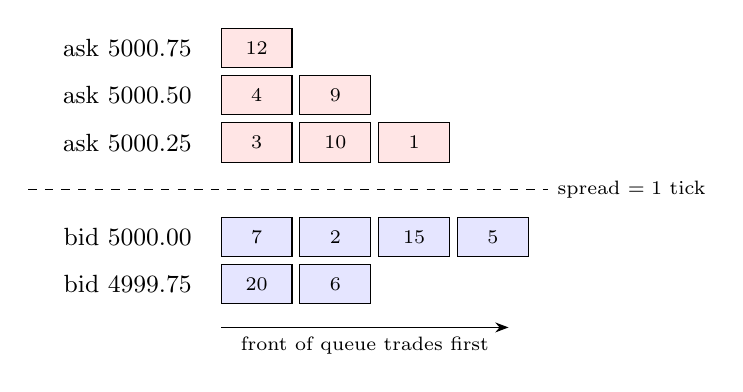
\begin{tikzpicture}[
  ord/.style={draw, minimum width=9mm, minimum height=5mm, font=\scriptsize, inner sep=1pt},
  px/.style={font=\small, anchor=east}]
\node[px] at (0,2.4) {ask 5000.75};
\node[px] at (0,1.8) {ask 5000.50};
\node[px] at (0,1.2) {ask 5000.25};
\node[px] at (0,0.0) {bid 5000.00};
\node[px] at (0,-0.6) {bid 4999.75};
\node[ord, fill=red!10] at (0.7,2.4) {12};
\node[ord, fill=red!10] at (0.7,1.8) {4};\node[ord, fill=red!10] at (1.7,1.8) {9};
\node[ord, fill=red!10] at (0.7,1.2) {3};\node[ord, fill=red!10] at (1.7,1.2) {10};\node[ord, fill=red!10] at (2.7,1.2) {1};
\node[ord, fill=blue!10] at (0.7,0.0) {7};\node[ord, fill=blue!10] at (1.7,0.0) {2};\node[ord, fill=blue!10] at (2.7,0.0) {15};\node[ord, fill=blue!10] at (3.7,0.0) {5};
\node[ord, fill=blue!10] at (0.7,-0.6) {20};\node[ord, fill=blue!10] at (1.7,-0.6) {6};
\draw[dashed] (-2.2,0.6) -- (4.4,0.6) node[right, font=\scriptsize] {spread $=1$ tick};
\draw[-{Stealth}] (0.25,-1.15) -- node[below, font=\scriptsize]{front of queue trades first} (3.9,-1.15);
\end{tikzpicture}
\caption{A small book. Each box is one waiting order and the number is its size in lots. Orders at
the same price form a first-in-first-out queue, front on the left. The best bid is 5000.00 with
$7+2+15+5 = 29$ lots; the best ask is 5000.25 with $14$ lots; the spread is one tick of 0.25.}
\label{fig:book}
\end{figure}

\paragraph{Queues and priority.}
Which waiting order trades first is decided by the venue's \emph{priority rule}. Most venues use
\emph{price--time priority}: better prices trade first, and among orders at the same price the one
that arrived first trades first. Each price level is then exactly a FIFO queue. Some products use
\emph{pro-rata} allocation instead, in which an incoming order is split among the waiting orders in
proportion to their sizes; at CME, for example, most futures match first-in-first-out while SOFR
interest-rate futures use a pro-rata or allocation algorithm~\citep{cme_matching}. Under
price--time priority an order's place in the queue matters, and the rules for keeping it matter
too: on CME Globex, decreasing an order's quantity keeps its place, while increasing the quantity
or changing the price sends it to the back of the queue~\citep{cme_matching}. The volume waiting
ahead of an order is its \emph{queue position}; much of this survey is about why that number
matters.

\paragraph{What a market-data feed shows.}
Exchanges publish the book through market-data feeds at three levels of detail. \emph{Level~1}
gives only the best bid and ask and their sizes. \emph{Level~2}, or \emph{market by price} (MBP),
gives the total size at each of the best few price levels. \emph{Level~3}, or \emph{market by
order} (MBO), reports every individual order: each addition, execution, cancellation and
modification, with an order identifier. MBO data provide the information needed to
reconstruct the displayed order-level queues, and therefore to estimate queue positions, subject to the
venue's matching rules and feed semantics; hidden liquidity and feed gaps remain outside what any feed
shows.

\paragraph{Example: building the book from Nasdaq ITCH.}
Nasdaq's TotalView-ITCH~5.0 feed is a widely used MBO protocol and a clear example of how a book is
built from messages~\citep{itch50}. Every message is a small fixed-layout binary record with a
one-character type, a timestamp in nanoseconds since midnight, and, for order messages, an 8-byte
\emph{order reference number} that identifies the order for the rest of the day. The order
messages are:

\begin{center}\footnotesize
\begin{tabular}{cll}
\toprule
Type & Name & Effect on the book \\
\midrule
\texttt{A}, \texttt{F} & Add Order & new order (side, shares, price) joins the back of its queue \\
\texttt{E} & Order Executed & order traded; reduce its shares by the executed amount \\
\texttt{C} & Order Executed With Price & as \texttt{E}, at a price different from the order's own \\
\texttt{X} & Order Cancel & partial cancel; reduce its shares \\
\texttt{D} & Order Delete & order cancelled; remove it \\
\texttt{U} & Order Replace & remove the old order; add a new one with a new reference number \\
\texttt{P} & Trade (non-cross) & an execution against a non-displayed order; no book change \\
\bottomrule
\end{tabular}
\end{center}

\noindent Building the book is a short event loop over these messages:
\begin{lstlisting}[language=Python]
book   = {'B': SortedDict(), 'S': SortedDict()}  # price -> deque of orders
orders = {}                                       # reference number -> order

def on_message(m):
    if m.type in 'AF':                            # add: join the back of the queue
        o = Order(m.ref, m.side, m.price, m.shares)
        book[o.side].setdefault(o.price, deque()).append(o)
        orders[o.ref] = o
    elif m.type in 'ECX':                         # execution or partial cancel
        o = orders[m.ref]
        o.shares -= m.shares
        if o.shares == 0: remove(o)
    elif m.type == 'D':                           # full cancel
        remove(orders[m.ref])
    elif m.type == 'U':                           # replace: remove, re-add at back
        old = orders[m.old_ref]
        remove(old)
        on_message(Add(m.new_ref, old.side, m.price, m.shares))

def remove(o):
    q = book[o.side][o.price]
    q.remove(o)                                   # O(1) with a linked list
    if not q: del book[o.side][o.price]
    del orders[o.ref]
\end{lstlisting}
Three details matter later in this survey. First, an execution message names the waiting order
that traded, so the feed reveals \emph{which} order in the queue was hit---the information needed
to reconstruct queue positions (Part~IV). Second, a replace carries a new reference number, so in
the reconstructed book the order leaves its place and rejoins at the back. Third, hidden orders
produce only \texttt{P} messages and never enter the book: the book a feed lets you build is the
\emph{displayed} book. ITCH is delivered over a sequenced UDP multicast protocol (MoldUDP64), so a
receiver can detect lost packets by gaps in the sequence numbers. CME's MDP~3.0 market-by-order feed,
used by the system in Part~IV, follows the same pattern with its own binary
encoding~\citep{cme_mdp3}.

At time $t$, an $L$-level description of the book is
\begin{equation}
  \mathcal{L}_t = \left\{ p^{b}_{\ell,t},\, v^{b}_{\ell,t},\, p^{a}_{\ell,t},\, v^{a}_{\ell,t}
  \right\}_{\ell=1}^{L},
\end{equation}
where $p^{b}_{\ell,t}$ and $v^{b}_{\ell,t}$ are the price and displayed volume at the $\ell$-th best
bid level ($\ell = 1$ is the best bid), and $p^{a}_{\ell,t}$, $v^{a}_{\ell,t}$ the same on the ask side.
\inwords{this is the market-by-price view of the book: a table with $L$ rows per side, each row a
price and the total number of lots waiting there. It can be computed from the order-level book by
summing each queue. It is the state of the market, and it changes every time an order arrives,
trades or is cancelled.}
The mid-price and
spread,
\begin{equation}
  m_t = \tfrac12\left(p^{a}_{1,t}+p^{b}_{1,t}\right), \qquad s_t = p^{a}_{1,t}-p^{b}_{1,t},
\end{equation}
\inwords{the mid $m_t$ is halfway between the best price anyone will buy at and the best price
anyone will sell at; it is the usual single-number ``price'' of the market. The spread $s_t$ is the
gap between them: buying and immediately selling back costs one spread.}
These are convenient summaries that discard most of the book: the distribution of liquidity across
levels, the sequence of events that produced the current state, and the queue position of any
individual order.

Throughout, numerical examples use stylised values chosen to make the arithmetic visible. They are
not empirical estimates, and this paper reports no new experiments.

\begin{example}[Same mid, different market]
Two E-mini S\&P 500 (ES) books have the same mid (5000.125) and the same one-tick spread (tick
$=0.25$). In the first, 12 lots rest at the best ask; in the second, 900. Buying 100 lots
aggressively costs several ticks more in the first book than in the second. Mid and spread do not
distinguish them.
\end{example}

Three properties make LOB modelling unusually hard. The data are \emph{event-driven}: orders arrive,
execute and cancel at irregular times. The state is \emph{high-dimensional} even when only a few
levels are observed. And the statistical properties are \emph{non-stationary} across time of day,
assets, volatility regimes and market-structure changes. A model that performs well for one
representation, horizon or market is therefore not, by that fact, a model of order-book dynamics.

\subsection{Notation}
\label{sec:notation}

This subsection fixes the symbols used throughout, and explains what each one means for a trader
watching the book. Symbols used in only one section are defined where they first appear. To make
the symbols concrete, each group is followed by its value in one running example: the book of
Figure~\ref{fig:book}, where at time $t$ we decide to place a passive buy order for one lot at
5000.00.

\begin{description}[leftmargin=1.5em,style=nextline,itemsep=4pt]
\item[Time and events]
  $t$ is time. Book events (additions, cancellations, executions) are numbered $n = 1, 2, \dots$
  and happen at times $t_1 \le t_2 \le \cdots$. A quantity written with subscript $t$ is its value
  just after everything that happened up to and including $t$; $t-$ means ``just before $t$''.
  $H > 0$ is a horizon---how far ahead we look---and $\delta$ is the tick size.\\
  \emph{What it means:} the market is a stream of events, and we look at it as a sequence of
  snapshots taken whenever we like. $H$ is the question ``how long am I willing to wait?''\\
  \emph{Example:} $\delta = 0.25$ (one ES tick), and we look $H = 1$ s ahead.

\item[Book]
  $p^{b}_{\ell,t}$, $v^{b}_{\ell,t}$, $p^{a}_{\ell,t}$, $v^{a}_{\ell,t}$, the mid $m_t$ and the
  spread $s_t$ are as defined in Section~\ref{sec:intro}. The change in the mid over the next $H$
  seconds is $\Delta m_{t,H} = m_{t+H} - m_t$.\\
  \emph{What it means:} $\Delta m_{t,H}$ is ``how much did the price go up (or down, if negative)
  while I waited''. Almost every prediction model in the literature targets some function of it.\\
  \emph{Example:} $p^b_{1,t} = 5000.00$, $v^b_{1,t} = 29$, $p^a_{1,t} = 5000.25$, $v^a_{1,t} = 14$,
  so $m_t = 5000.125$ and $s_t = 0.25$. If one second later the best bid and ask are 4999.75 and
  5000.00, then $m_{t+H} = 4999.875$ and $\Delta m_{t,H} = -0.25$: the price fell one tick.

\item[Information and prediction]
  $X_t$ is everything observable at $t$ that a model may use: the book, recent events, and anything
  derived from them. $Y_{t+H}$ is the quantity we want to predict, which becomes known only at
  $t+H$; $\widehat{Y}_t$ is a model's prediction of it, made at $t$.\\
  \emph{What it means:} $X_t$ is the model's input vector and $\widehat{Y}_t$ its output. The rule
  is that $X_t$ may contain only what was really known at $t$---no peeking at the future.\\
  \emph{Example:} $X_t$ could be the sizes of the five best levels on each side; $Y_{t+H}$ could be
  ``did the mid rise within one second?'', and $\widehat{Y}_t = 0.6$ a model's estimate that it
  will.

\item[Actions and orders]
  $a_t$ is what we do at $t$: place an order, keep it, cancel it, or cross the spread. $d$ is the
  side of an order, $d = +1$ for a buy and $d = -1$ for a sell. For a waiting order,
  $Q^{\text{ahead}}_t$ is the displayed volume ahead of it in its queue, and $q$ stands for a
  particular value of $Q^{\text{ahead}}_t$.\\
  \emph{What it means:} $d$ lets one formula serve both buyers and sellers, since a rising price is
  good for a buyer and bad for a seller. $Q^{\text{ahead}}_t$ is ``how many people are in line in
  front of me''.\\
  \emph{Example:} $a_t$ = place a bid at 5000.00, $d = +1$. The new order joins the back of the
  5000.00 queue, so $Q^{\text{ahead}}_t = 29$.

\item[Fills]
  $\tau_F$ is how long after $t$ the order is filled ($\tau_F = \infty$ if it never is),
  $t_F = t + \tau_F$ is the clock time of the fill, and $p^{\text{fill}}$ is the price received.
  $\Fill$ is the event ``the order was filled within the horizon'', $\{\tau_F \le H\}$, and
  $\mathbb{1}_{\Fill}$ is $1$ if that happened and $0$ otherwise.\\
  \emph{What it means:} a passive order is a bet that someone will come and trade with it; these
  symbols record whether, when and at what price they did.\\
  \emph{Example:} sellers trade through the whole 5000.00 queue 0.4 s later and reach our order:
  $\tau_F = 0.4$ s, $p^{\text{fill}} = 5000.00$, and since $0.4 \le 1$, $\mathbb{1}_{\Fill} = 1$.

\item[Profit]
  $\Pi$ is the profit per lot of an order decided at $t$, in price points unless stated otherwise
  (some examples use ticks); it is defined precisely in Section~\ref{sec:passive}. A passive order
  that is never filled makes $\Pi = 0$. $h > 0$ is the \emph{mark-out horizon}: how long after a
  fill we wait before scoring it.\\
  \emph{What it means:} $\Pi$ is the number we actually care about; every other symbol is a step
  on the way to it.\\
  \emph{Example:} with $h = 1$ s, if the mid one second after our fill is 4999.875, our buy at
  5000.00 is worth $4999.875 - 5000.00 = -0.125$: we were filled, and then the price moved against
  us. This is \emph{adverse selection} (Section~\ref{sec:adverse}), and it is why a fill is not
  automatically good news.

\item[Models]
  $M$ denotes a model, $M_0$ a baseline (usually the simplest reasonable one) and $M_1$ a candidate.
  $V(M)$ is how much money-relevant value $M$ delivers \emph{out of sample} (OOS)---on data that were
  not used to build it, as opposed to \emph{in sample}---for example net profit after costs, or a Sharpe ratio (average return divided
  by the standard deviation of return~\citep{sharpe1994}). $\Delta V = V(M_1) - V(M_0)$.\\
  \emph{What it means:} $\Delta V$ answers ``is the new model worth it, compared with the simple
  one, on data it has never seen?''\\
  \emph{Example:} if a linear model earns 0.010 points per trade after costs and a neural network
  earns 0.012, then $\Delta V = 0.002$ points per trade; Principle~3 below asks whether that is
  real and whether it pays for the extra complexity.

\item[Operators]
  $\P$ is ``the probability of'', $\E$ is ``the average of'', and a vertical bar means ``given''.
  Section~\ref{sec:primer} explains these in plain terms.
\end{description}

\subsection{A short probability primer}
\label{sec:primer}

Most equations in this paper are statements about probabilities and averages. The few ideas needed
are the following; a first course in probability covers all of them.

\begin{description}[leftmargin=1.5em,style=nextline,itemsep=2pt]
\item[{$\P(A)$, ``the probability of $A$''}] A number between 0 and 1: the fraction of times event
  $A$ would happen if the situation were repeated many times. Example: $\P(\Delta m_{t,H} > 0)$ is
  the fraction of moments after which the mid is higher $H$ seconds later.
\item[{$\P(A \mid B)$, ``the probability of $A$ given $B$''}] The same fraction, but counted only
  over the cases where $B$ is true. The vertical bar is read ``given''. Example:
  $\P(\Delta m_{t,H} > 0 \mid \text{bid queue much larger than ask queue})$ asks: of all the moments
  when buyers were queued much more heavily than sellers, what fraction were followed by a rise?
  Writing $\mid X_t$ means ``given everything we can observe at time $t$''---it is what a
  prediction model computes: a function from the current inputs $X_t$ to a probability.
\item[{$\E[Z]$, ``the expected value of $Z$''}] The long-run average of a random number $Z$. If a
  trade makes $+2$ with probability $0.6$ and $-1$ with probability $0.4$, then
  $\E[Z] = 0.6 \times 2 + 0.4 \times (-1) = 0.8$.
\item[{$\E[Z \mid B]$}] The average of $Z$ over only the cases where $B$ is true.
\item[{$\mathbb{1}_A$, the indicator of $A$}] Equal to $1$ if $A$ happens and $0$ otherwise, like a
  Boolean cast to an integer. Its average is the probability: $\E[\mathbb{1}_A] = \P(A)$. A useful
  consequence, used in Section~\ref{sec:passive}, is
  $\E[Z\,\mathbb{1}_A] = \P(A)\,\E[Z \mid A]$: the average of ``$Z$ if $A$ happened, else 0'' equals
  how often $A$ happens times the average of $Z$ when it does.
\item[{$\inf\{u > 0 : \text{condition}\}$}] ``The earliest time $u$ after now at which the condition
  holds''---the time a \texttt{while} loop that polls the condition would exit.
\item[{A hat, as in $\widehat{Y}_t$}] An estimate produced by a model, as opposed to the true value.
\end{description}

\subsection{Prediction versus tradeability}
\label{sec:tradeability}

Suppose a model estimates $\P(\Delta m_{t,H} > 0 \mid X_t)$, the probability that the mid rises over
the next $H$. That
number describes directional predictability. It does not say whether a trader can monetise it. An
aggressive buy pays the offer and must overcome the half spread and fees. A passive buy avoids the
spread but may never execute, and the event that makes it execute may itself carry information
about the next price move. The economically relevant sequence is
\begin{equation}
  \begin{gathered}
  X_t \;\to\; \widehat{Y}_t \;\to\; a_t \;\to\; \text{placement} \;\to\; \text{queue position}\\
  \;\to\; \text{execution} \;\to\; \text{realised profit and loss (P\&L)}.
  \end{gathered}
  \label{eq:chain}
\end{equation}
\inwords{data go into a model; the model makes a forecast; the forecast is turned into a decision
(buy, sell, wait, cancel); the decision becomes an order; the order takes a place in a queue;
whether and when it trades depends on that place; and only then is money made or lost. A forecast
can be right and still be lost at any later arrow.}

\begin{example}[Accurate but untradeable]
\label{ex:untradeable}
In ES (tick $0.25$ points, one-tick spread), a classifier is right on the sign of the next mid
move 55\% of the time, and the typical move is half a tick ($0.125$ points). The expected move per
trade in the predicted direction is
\[
  (0.55 - 0.45)\times 0.125 = 0.0125 \text{ points},
\]
while an aggressive entry costs the half spread, $0.125$ points, before fees. The expected directional edge is
one tenth of the half-spread cost, before fees, so it does not cover even the cost of entry. The accuracy is real, and the strategy loses money. The same signal used to decide
\emph{which resting passive order to keep and which to cancel} pays no spread; whether it helps is
an execution question (Part~III), not an accuracy question.
\end{example}

A related line of work asks not only for a forecast but for a measure of \emph{when the forecast
can be trusted}. UQ-LOB~\citep{manoharan2026uqlob} attaches an uncertainty module to a pretrained
LOB encoder and outputs a \emph{calibrated} distribution---one whose stated probabilities match
observed frequencies, so that events given 70\% happen about 70\% of the time~\citep{guo2017}---with
a scalar confidence. Restricting attention to the most confident tenth (\emph{decile}) of
predictions raises directional macro-F1 by 0.11--0.15 in its regression variant (F1 is the harmonic
mean of precision and recall; \emph{macro}-F1 averages it over the classes ``up'', ``down'' and
``stationary''), across seven cryptocurrency assets at 5, 10 and 15 second horizons. Selective
prediction changes the tradeability arithmetic directly: if a confident tier moved accuracy from
55\% to 70\% on a tenth of the signals, the expected edge per trade in
Example~\ref{ex:untradeable} would rise from $0.10$ to $0.40$ of the typical move, with one tenth
as many trades. Whether that clears the half spread still depends on the size of the moves in the
confident tier. UQ-LOB itself stops at directional reliability: its authors state that they
evaluate reliability, not profitability, and that a trading simulation with realistic execution
and fees is required before any claim about returns~\citep{manoharan2026uqlob}. That is the step
this survey is about.

This is the central question of the survey:

\begin{quote}
\emph{Which information extracted from the limit order book survives the complete translation from
statistical prediction to executable trading?}
\end{quote}

It changes how models should be compared. A model that improves classification accuracy by a
fraction of a percentage point is not more useful than a linear model if the improvement vanishes
after latency and costs. A model with modest directional accuracy may still be valuable if it
improves the timing or selection of passive executions.

\subsection{Prediction, execution and simulation are different problems}
\label{sec:three-problems}

LOB research frequently mixes up three different questions. Each is written below as a
probability or an expected value (Section~\ref{sec:primer}). The big $\P$ is ``the probability
of'', $\E$ is ``the average of'', and the vertical bar is read ``given'': everything to the right of
the bar is what we already know, everything to the left is what we want to know.
\begin{align}
  \text{Prediction:} &\quad \P(Y_{t+H} \mid X_t), \\
  \text{Execution:}  &\quad \P(\Fill \mid X_t, Q^{\text{ahead}}_t, a_t)
                        \ \text{or}\ \E[\Pi \mid X_t, Q^{\text{ahead}}_t, a_t], \\
  \text{Simulation:} &\quad \P\big(\{X_u\}_{u \in (t,\,t+H]} \mid X_t\big).
\end{align}
\inwords{
\begin{itemize}[leftmargin=1.5em,itemsep=1pt]
\item \emph{Prediction}~(4): given what we can see now, how likely is each possible value of some
  future quantity $Y$---for example, ``will the mid be higher in one second?'' It is a question
  about the market, and our own orders play no part in it.
\item \emph{Execution}~(5): given what we can see now, how much volume is ahead of our order, and
  what we chose to do, how likely is our order to be filled within $H$ seconds---or, in the second
  form, how much do we expect to earn? It is a question about \emph{our} order, and its answer
  changes with our action $a_t$.
\item \emph{Simulation}~(6): given what we can see now, how likely is each possible \emph{whole
  future path} of the market over the next $H$ seconds? A simulator draws sample paths from this
  distribution. The difference from~(4) is the difference between a weather simulator, which
  produces whole plausible tomorrows, and a forecast of tomorrow's maximum temperature.
\end{itemize}}
Two different activities are both called ``simulation'' in this literature, and the survey keeps them
apart. \emph{Generative market simulation} draws new market paths from a model of~(6): Hawkes
simulators, agent-based markets and the generative networks of Section~\ref{sec:deep-gen}.
\emph{Historical replay} does not draw paths at all: it reconstructs the one path that was recorded,
event by event, and evaluates the counterfactual outcome of the researcher's own orders against it---an
estimate of~(5) on observed data. The Kaspar system of Part~IV is a replay system, not a generative
simulator.
They are related but not interchangeable. A Hawkes process can generate realistic clustered order
flow without producing directional alpha. A survival model can give accurate fill probabilities
while playing no role in price prediction. A Transformer can predict short-horizon returns without
modelling queue dynamics. Each model must be evaluated against the problem it solves.

\begin{table}[ht]
\centering\small
\caption{One event stream (a day of ES market-by-order data), three models, three evaluation
criteria. Using the wrong column is a common source of misleading comparisons.}
\label{tab:three-problems}
\begin{tabularx}{\linewidth}{lXXX}
\toprule
Model & Target & Appropriate metric & Inappropriate metric \\
\midrule
Hawkes, 4 event types & event intensity & point-process log-likelihood; time-rescaling residual test & directional accuracy \\
Survival model & $\P(\tau_F \le 1\,\mathrm{s} \mid Q^{\text{ahead}}_t = q)$ & survival likelihood; calibration by queue bucket & mid-move AUC \\
Classifier & $\P(\Delta m_{t,H} > 0 \mid X_t)$ & log loss, AUC, then net P\&L & fill rate \\
\bottomrule
\end{tabularx}
\end{table}

\subsection{Three fixed positions}

Three positions recur throughout the paper.

\begin{principle}[The market is observed, not generated]
Recorded exchange data are the ground truth. A replay simulator reconstructs the historical book
from those data; it does not invent market behaviour. The only counterfactual it produces is the
execution outcome of the researcher's own orders.
\end{principle}

\begin{principle}[Language models generate hypotheses, not data]
In LLM-assisted model discovery the language model proposes candidate models. Fitting, replay,
validation and certification are carried out outside the language model, by fixed procedures that are
reproducible given the same data, configuration and random seeds. The language model does not generate
the market data used as evidence.
\end{principle}

\begin{principle}[Occam's razor: complexity is an empirical hypothesis]
Among models that deliver the same out-of-sample economic value, prefer the simplest. Each added
layer---model capacity, specialised hardware, and the breadth of the search that produced the
model---is a hypothesis that it adds value, and must earn incremental out-of-sample economic value
that survives realistic execution assumptions and the multiple-testing burden of its own selection.
\end{principle}

\noindent Occam's razor is applied here to economic value, not to statistical fit alone: a more
complex model is not rejected for being complex, but it carries the burden of showing that its
extra value is real. Section~\ref{sec:parsimony} makes this operational.

\subsection{How the field developed}
\label{sec:history}

The modelling of order books has passed through five overlapping stages.
\begin{enumerate}[leftmargin=1.8em,itemsep=2pt]
\item \textbf{Zero-intelligence models.} Orders arrive at random, with no strategy at all, and the
  matching rules do the rest~\citep{smith2003}. The surprise was how much this explains: on eleven
  London stocks, a model with one free parameter accounts for 96\% of the variance of the bid--ask
  spread~\citep{farmer2005}. Market structure, not trader intelligence, explains much of what the book
  looks like.
\item \textbf{Stochastic queue models.} The best queues are treated as random walks driven by order
  arrivals, cancellations and executions, giving closed-form results for the time to the next price
  change and the probability of its direction~\citep{cst2010,contlarrard2013}, later with rates that
  depend on queue sizes~\citep{huang2015}.
\item \textbf{Self-exciting point processes.} Hawkes models capture the clustering of events and the
  fact that many events are triggered by earlier ones; estimated branching ratios on E-mini S\&P data
  range from about $0.7$--$0.8$ to about one~\citep{bacry2015,filimonovsornette2012,hardimanbercotbouchaud2013}.
\item \textbf{Hand-engineered signals.} Order-flow imbalance~\citep{cks2014}, queue
  imbalance~\citep{gould2016qi} and the micro-price~\citep{stoikov2018} compress the book into a few
  numbers with clear economic meaning.
\item \textbf{Learned models.} From 2017, convolutional and recurrent networks~\citep{tsantekidis2017,zhang2019},
  then attention and spatial-temporal Transformers~\citep{wallbridge2020,berti2025tlob}, then pretrained
  message-level encoders and large generative models~\citep{linna2025lobert,m3lob}, together with
  hybrids that put point-process structure inside networks~\citep{shi2022sdpnhp,deepqr}.
\end{enumerate}
Each stage added capacity. Whether each also added \emph{economic} value is the question this survey
keeps asking.

\subsection{Positioning and taxonomy}
\label{sec:taxonomy}

The literature has three historical traditions. The first is econometric and reduced-form
modelling of prices, order flow and impact~\citep{kyle1985,glosten1985,cks2014}. The second is
continuous-time point-process and queueing models: Hawkes processes preserve the event-driven
structure and model excitation between event types~\citep{hawkes1971,bacry2015}, while
queue-reactive and first-passage models describe displayed liquidity and its
depletion~\citep{cst2010,huang2015}. The third is machine learning, from hand-engineered features
through CNNs, recurrent networks, Transformers, state-space models and, most recently, pretrained
message-level encoders~\citep{tsantekidis2017,zhang2019,wallbridge2020,linna2025lobert}.

\paragraph{Position relative to existing surveys.} Existing surveys and books cover parts of this
ground well (Table~\ref{tab:prior-surveys}): the LOB as a trading mechanism and its empirical
literature~\citep{gould2013,tripathi2020}, machine-learning prediction from the
book~\citep{zaznov2022}, generative simulation of order books~\citep{jain2024sim}, and, more recently,
large language models and autonomous agents in financial
trading~\citep{ding2024llmtrading,dong2025llmfinance,hua2026agentic}. These works provide taxonomies of
models and applications, but generally treat LOB modelling, trading prediction, execution and queue
position, market simulation, and automated hypothesis search as separate topics. We are not aware of a
survey that brings these strands together around the question of how information extracted from the
LOB survives the complete translation from statistical prediction to executable trading. That question
is also this survey's criterion for selecting literature: a model or method is included when it bears
on one link of the chain---representation, prediction, calibration, decision, queue position,
execution, replay, economic value, model search and multiple testing, and LLM-assisted hypothesis
generation. The individual subjects are not new; the integration, and the criterion that connects
them, are. Two distinctions follow from it and recur throughout: historical replay is distinguished
from generative market simulation, and language models are treated as generators of hypotheses, not
as sources of market data or of validation.

\paragraph{Generative LOB simulation versus historical replay.} The closest neighbouring review, on
LOB simulation~\citep{jain2024sim}, classifies, by methodology, models that \emph{generate} order-book dynamics, and evaluates them by their ability
to reproduce stylised facts and price impact. That is one of two legitimate ways of using a simulator,
and they answer different questions:
\begin{itemize}[leftmargin=1.5em,itemsep=1pt]
\item \emph{generative simulation} asks whether a model can produce plausible market trajectories,
  including ones never observed, such as stress scenarios;
\item \emph{historical replay} asks what would have happened to a particular strategy's orders against
  one observed trajectory.
\end{itemize}
To decide whether an order would have executed against the historical market, the market does not
need to be generated, only reconstructed. This survey is concerned primarily with the second question;
generative models are covered in Section~\ref{sec:deep-gen} as tools for simulation and stress testing.

\paragraph{Language models: hypothesis generator, not trading agent.} The surveys of LLMs in trading
review systems in which the language model reads market information, reasons about it and produces
trading decisions that are then backtested~\citep{ding2024llmtrading,hua2026agentic}. This survey does not
review that architecture. In the loop of Part~V the language model proposes a candidate model from a
fixed vocabulary of primitives; in the worked implementation it never receives market
prices~\citep{mayeski_latss}. Data enter only when an external, reproducible research engine compiles
the candidate, fits it, evaluates it out of sample and corrects for the number of candidates tried. The
implementation described there works on daily data; for order-book strategies the design adds replay
of each candidate's orders against the recorded book, which is the role of Part~IV.

The purpose here is therefore not another catalogue of architectures, but an organisation of the
literature around the translation from information to decision. Three questions recur: what representation contains the useful information;
what model extracts it; and does the result produce incremental economic value after execution
constraints?

\begin{table}[ht]
\centering\footnotesize
\caption{Existing surveys, books and benchmark studies, and what this survey adds.}
\label{tab:prior-surveys}
\begin{tabularx}{\linewidth}{>{\raggedright\arraybackslash}p{0.26\linewidth}>{\raggedright\arraybackslash}X>{\raggedright\arraybackslash}X}
\toprule
Work & Focus & Not covered there \\
\midrule
\citet{gould2013} & empirical facts and models of LOBs & deep learning; execution value; queue position in practice \\
\citet{abergel2016}, \citet{bouchaud2018} & books on empirical properties, models and simulation of order books and impact & recent deep and generative models; model-search statistics \\
\citet{tripathi2020} & systematic review of 103 articles (1981--2018) on the LOB as a trading mechanism and its implications for market efficiency, classified by sub-area, market, method and LOB measure & deep-learning prediction (named there only as a future direction); execution value; queue position \\
\citet{jain2024sim} & review of LOB simulation models and the stylised facts used to validate them & prediction and trading value \\
\citet{ding2024llmtrading}, \citet{dong2025llmfinance}, \citet{hua2026agentic} & surveys of LLMs as trading and financial agents: architectures, inputs, workflows, benchmarks, backtests, deployment & LOB microstructure; separation of hypothesis generation from evidence \\
\citet{zaznov2022} & survey of price-change prediction from the LOB & classical point-process and queue models; execution \\
\citet{prata2024}, \citet{briola2024} & benchmark re-tests of deep models; transaction-level evaluation & classical models; queue position; search statistics \\
This survey & information-to-decision chain: classical and deep models, queue position, deterministic replay, automated model discovery, evaluation & -- \\
\bottomrule
\end{tabularx}
\end{table}

\paragraph{Contributions.} The survey offers:
\begin{enumerate}[leftmargin=1.8em,itemsep=1pt]
\item a single chain---representation, prediction, decision, queue, execution, profit---that places
  classical and learned models in one framework;
\item a treatment of queue position, fill probability and adverse selection as modelling targets in
  their own right, with the signal-value/execution-value distinction (Section~\ref{sec:tradeability-framework});
\item a description of queue-exact deterministic replay as the evaluation instrument for execution
  claims (Part~IV);
\item an account of LLM-assisted model discovery as a statistical search process (Part~V);
\item evaluation standards that combine proper scoring, economic metrics, temporal validation and
  search-aware significance (Part~VI);
\item a reader-oriented apparatus: notation, a probability primer, plain-language explanations of every
  equation, a glossary and a point-process appendix.
\end{enumerate}

\paragraph{How to read this survey.} Readers new to markets should read Part~I in full and use the
glossary. Readers interested mainly in models should read Part~II, then Section~\ref{sec:benchmarks-dl}.
Practitioners concerned with execution should read Parts~III and IV and Section~\ref{sec:parsimony}.
Readers interested in automated research should read Parts~V and VI. The appendix on point processes
supports Section~\ref{sec:hawkes}.

\subsubsection*{Four axes for locating a piece of work}

Every model or paper in this survey answers four separate questions, and we describe it by its
answer to each. Think of the four answers as the four fields of a record; a work is a point in a
four-dimensional space.

\begin{description}[leftmargin=1.5em,style=nextline,itemsep=2pt]
\item[Representation: what does the model see?] The input format: raw book snapshots (the table
  of Equation~(1) at sampled times); event or message streams (every add, cancel and trade, in
  order); order-flow aggregates such as OFI (Section~\ref{sec:ofi}); queue state (sizes and
  positions in the queues); or the state of several instruments at once.
\item[Model class: what kind of function maps input to output?] Linear and econometric models;
  queue and first-passage models; point processes such as Hawkes; state-space models; convolutional
  and recurrent networks; Transformers; pretrained encoders; or a hybrid of these.
\item[Objective: what quantity does it output?] Price direction; return; event intensity;
  volatility; queue depletion time; fill probability; execution cost; or a simulated future.
\item[Economic role: what decision is the output for?] Aggressive trading (crossing the spread);
  passive trading (resting orders); market making (quoting both sides); execution of a given
  order; risk measurement; or simulation for research. A paper that evaluates only statistical
  accuracy and names no decision has an \emph{unspecified} economic role.
\end{description}

\noindent The axes are used in three ways.

\emph{First, to decide what can be compared.} Two results are comparable only if they share an
objective and an economic role, and in addition the data fields of Section~\ref{sec:comparable}.
Representation and model class are the things a study varies; objective and role are the things
it must hold fixed. A Hawkes model scored on event-intensity likelihood and a Transformer scored on
direction accuracy are not competitors, however often they appear in the same table.

\emph{Second, to organise the paper.} Part~II moves along the model-class axis, from linear models
to pretrained encoders, and Section~\ref{sec:events} along the representation axis. Part~III moves
along the objective axis from direction to fill probability and adverse selection. Parts~IV and V
fix the economic role---passive execution---and ask what each objective is worth for it.

\emph{Third, to expose a gap.} Table~\ref{tab:axes} places the main works discussed in this survey
on the four axes. The economic-role column is where the literature is thinnest: many of the
learned models are evaluated on accuracy alone, and the decision their output would drive is left
unspecified. The rest of the paper is about filling that column.

\begin{table}[ht]
\centering\footnotesize
\caption{Selected works placed on the four axes. ``Unspecified'' means the work evaluates
statistical accuracy without stating or evaluating a trading decision. \pov{} (Shadow Passive
Percentage-of-Volume) is the model-free execution algorithm of Section~\ref{sec:shadow}.}
\label{tab:axes}
\setlength{\tabcolsep}{2pt}
\begin{tabularx}{\linewidth}{l*{4}{>{\raggedright\arraybackslash}X}}
\toprule
Work & Representation & Model class & Objective & Economic role \\
\midrule
OFI~\citep{cks2014} & order-flow aggregate & linear & contemporaneous price change & price impact (execution) \\
Book dynamics~\citep{cst2010} & queue state & queueing / first passage & direction; queue depletion & market making, execution \\
Queue-reactive~\citep{huang2015} & queue state & queueing (Markov) & event intensity & simulation \\
Hawkes models~\citep{bacry2015} & event stream & point process & event intensity & simulation, risk \\
Queue value~\citep{moallemi2017} & queue state & queueing & value of a queue position & passive trading, market making \\
DeepLOB~\citep{zhang2019} & raw snapshots & CNN + recurrent & direction & aggressive trading (simple trading simulation) \\
TransLOB~\citep{wallbridge2020} & raw snapshots & Transformer & direction & unspecified \\
Deep OFI~\citep{kolm2023} & order-flow aggregate & recurrent / feed-forward & return, several horizons & unspecified (scored by out-of-sample variance explained) \\
LOBERT~\citep{linna2025lobert} & event stream & pretrained encoder & direction; next message & unspecified \\
UQ-LOB~\citep{manoharan2026uqlob} & event stream & encoder + uncertainty module & direction with confidence & unspecified (stated by the authors) \\
\pov{}~\citep{maciejewski_shadow} & event stream & none (rule) & execution cost & passive execution \\
\bottomrule
\end{tabularx}
\end{table}

% ================================================================
\section{Survey methodology}
\label{sec:method}
% ================================================================

A survey makes many claims, drawn from many papers that were written for different purposes. This
section explains what the survey covers, how its sources were chosen, how strongly each kind of
claim should be believed, and what has to be known about two studies before their numbers can be
compared. The last part is a practical checklist for reading any paper in this field.

\subsection{Scope: which markets and which questions}

The survey covers limit order books in four kinds of market. They share the mechanism of
Section~\ref{sec:intro} but differ in ways that change what a model can learn and whether a result
carries over from one to another.

\begin{table}[ht]
\centering\small
\caption{The markets covered, and how they differ in ways that matter for LOB models.}
\label{tab:markets}
\begin{tabularx}{\linewidth}{l*{3}{>{\raggedright\arraybackslash}X}}
\toprule
Market & How it trades & Typical data & What it means for models \\
\midrule
Futures (e.g.\ ES, NQ, ZN) & Each contract trades on one exchange, in nearly continuous sessions &
  Exchange MBO feeds such as CME MDP~3.0 & One book holds all the liquidity, so the book a model
  sees is the whole market. \\
US equities & The same stock trades on many exchanges and off-exchange venues at once & Exchange
  feeds such as ITCH, one venue at a time & One venue's book is only part of the market; flow
  elsewhere moves prices too. \\
Cryptocurrencies & Many independent exchanges, open 24 hours a day, every day & Public exchange
  APIs, often snapshots plus updates & Data are easy to obtain, but fees, participants and trading
  hours differ from traditional markets. \\
Fixed income & Government bond futures on futures exchanges; cash bonds on electronic
  inter-dealer platforms & Varies by venue & Treasury futures are large-tick instruments: the price rarely
  moves by more than a tick, queues are long, and queue position matters. \\
\bottomrule
\end{tabularx}
\end{table}

Within these markets the survey includes work whose main object is one of four things:
\emph{prediction} (forecasting prices or events), \emph{signal extraction} (building features from
the book), \emph{execution} (deciding how to place, keep and cancel orders), or \emph{simulation}
(reproducing the market for research). Two adjacent areas are deliberately left out. Equilibrium
models, which derive prices from the optimal behaviour of rational traders, and agent-based models,
which simulate many rule-following traders, appear only where they help explain an LOB model; they
are not fitted to the data the rest of the paper is about. Synthetic market data produced by
learned generative models are discussed in Section~\ref{sec:three-uses}, but, following Principle~1,
they play no part in the methodology the survey recommends.

\subsection{How the sources were chosen}

This is a \emph{narrative} survey, not a \emph{systematic review}. A systematic review fixes a
search query and a list of databases in advance, screens every result against written criteria, and
reports how many papers were kept at each step, so another team could repeat the search exactly. A
narrative survey instead selects work that illustrates and tests an argument. That is appropriate
here, because the aim is to organise the field around one question---what survives the translation
from prediction to execution---rather than to count papers. It also has a known weakness: the
selection may favour work that fits the argument. To limit that, the survey includes work that cuts
against its own position where such work exists, for example evidence that deep models given
suitable inputs reach state-of-the-art predictive accuracy (Section~\ref{sec:deep}).

A work was included if it made at least one of the following contributions: a representation of the
order book; a predictive model; a queue or execution model; an evaluation method; a public data set
or benchmark; or a design for simulation or research infrastructure. Preference was given to
peer-reviewed work and to widely cited preprints; recent preprints are included when they are the
only source for an idea, and are identified as preprints in the bibliography. Every reference was
checked against the publisher, the preprint server or the official documentation.

\subsection{How strongly to believe a claim}

Not all statements in a survey deserve the same confidence. We distinguish four kinds, and the
reader should ask of every claim which kind it is.

\begin{description}[leftmargin=1.5em,style=nextline,itemsep=3pt]
\item[Established result] Supported directly by a cited study, or true by mathematics.
  \emph{Example:} a linear Hawkes process is stationary if and only if the cascade of events it
  triggers dies out (Section~\ref{sec:hawkes})
  (Section~\ref{sec:hawkes}). This is a theorem; no data can overturn it.
\item[Empirical synthesis] A conclusion drawn by comparing several studies, none of which tested it
  directly. \emph{Example:} ``the input representation can matter as much as the architecture''
  (Section~\ref{sec:deep}). It rests on a pattern across papers, so it can be wrong for a market
  those papers did not study.
\item[Methodological recommendation] A proposed standard, argued for rather than proved.
  \emph{Example:} every result should report how many model configurations were tried
  (Section~\ref{sec:search}). Its justification is a statistical argument, not a measurement.
\item[Open hypothesis] Plausible, but the evidence is incomplete or conflicting. \emph{Example:}
  adding Hawkes intensities to a large network that already sees the same events adds little value
  (Section~\ref{sec:hybrid}). The survey argues for it; nobody has shown it.
\end{description}

\noindent The distinction matters because LOB studies differ in assets, horizons, targets and data,
and a result established under one set of conditions is at best a hypothesis under another.
Table~\ref{tab:evidence} in Section~\ref{sec:conclusion} classifies the main claims of this paper
in these terms.

\subsection{What makes two LOB studies comparable?}
\label{sec:comparable}

Papers in this field routinely report a single headline number---an accuracy, an F1 score, a
Sharpe ratio---and readers routinely compare those numbers across papers. Such comparisons are
meaningful only when the studies agree on the conditions that produced the numbers.
Table~\ref{tab:comparable} lists the conditions that matter most and explains how each one can
change the headline number on its own, with no change to the model.

\begin{table}[ht]
\centering\small
\caption{Fields a study must report before its results can be compared with another's.}
\label{tab:comparable}
\begin{tabularx}{\linewidth}{>{\raggedright\arraybackslash}p{0.27\linewidth}>{\raggedright\arraybackslash}X}
\toprule
Field & Why it changes the result \\
\midrule
Asset, exchange, period, trading hours & Markets differ (Table~\ref{tab:markets}); the same market
  differs between calm and volatile years and between the open, midday and the close. \\
Tick size, typical spread, depth & A large tick makes mid changes rarer and queues longer, which
  changes both what is predictable and what is tradeable. \\
Message rate & A busy instrument produces many events per second; a horizon of ten events is a few
  milliseconds in one market and minutes in another. \\
Data level (L1, L2, L3) & Only L3 data reveal the causes of book changes and queue positions
  (Section~\ref{sec:events}). \\
Sampling clock & An \emph{event clock} samples after a fixed number of events, a \emph{calendar clock}
  after a fixed number of seconds. The event clock over-represents busy periods, which behave differently. \\
Horizon and target & Predicting the sign of the next mid change is a different problem from
  predicting a move larger than a threshold, or a return over ten seconds
  (Section~\ref{sec:deep}). \\
Class balance & If most samples belong to one class, a model that always predicts that class
  scores high accuracy while knowing nothing (Example~\ref{ex:imbalance}). \\
Train/test protocol & A random split lets the model train on data from after its test period; a
  chronological split does not (Section~\ref{sec:validation}). \\
Costs, latency and execution model & The same forecast is profitable or unprofitable depending on
  whether the spread, fees and delays are counted (Section~\ref{sec:tradeability}). \\
Number of configurations tried & The best of many tries looks good by chance
  (Section~\ref{sec:search}). \\
\bottomrule
\end{tabularx}
\end{table}

\begin{example}[Accuracy without knowledge]
\label{ex:imbalance}
A three-class target labels each sample ``up'', ``down'' or ``stationary'' according to whether
the mid moves by more than a threshold within the horizon. Suppose that, with a short horizon on a
large-tick future, 80\% of samples are ``stationary'', because the mid rarely moves at all. A model
that ignores its input and always answers ``stationary'' is then 80\% accurate. A genuinely useful
model might be 75\% accurate and still be better, because it is right on some of the up and down
moves that are the only cases a trader cares about. Accuracy alone cannot show this; balanced
accuracy, macro-F1 or the confusion matrix (the table of predicted against actual classes) can.
\end{example}

\begin{example}[Two ``65\% accuracy'' results]
One study reports 65\% on FI-2010~\citep{ntakaris2018}: five Nasdaq Nordic stocks, ten trading
days, a horizon of $10$ in the data set's own sampling units, three classes. Another reports 65\% on a cryptocurrency pair sampled
on a one-second calendar clock with two classes. With two balanced classes, 50\% is what guessing
achieves; with three classes, guessing achieves anywhere from 33\% to the share of the largest
class. The two numbers sit on different scales and share almost none of the fields of
Table~\ref{tab:comparable}. Their equality carries no comparative information.
\end{example}

\subsection{A reader's checklist}

The following questions can be asked of any paper in this field, including this one. A study that
cannot answer them has not yet shown that its result is useful for trading.

\begin{enumerate}[leftmargin=1.8em,itemsep=2pt]
\item \textbf{What exactly is predicted, over what horizon, on what clock?} (Section~\ref{sec:deep})
\item \textbf{What does a trivial model score on the same data?} Always guessing the most common
  class, or a linear model on order-flow imbalance (Section~\ref{sec:ofi}).
\item \textbf{Was the test period strictly after the training period?} (Section~\ref{sec:validation})
\item \textbf{How many models or settings were tried before this one was reported?}
  (Section~\ref{sec:search})
\item \textbf{What decision would the prediction drive, and was that decision evaluated after
  spread, fees and latency?} (Sections~\ref{sec:tradeability} and~\ref{sec:passive})
\item \textbf{If the decision uses passive orders, how were fills decided?} A fill rule that ignores
  the queue overstates results (Section~\ref{sec:replay}).
\end{enumerate}



\part{Models of the Limit Order Book}
\paragraph{About this part.} Part~II surveys the models of the order book, from the simplest to the
most complex. It starts with the empirical facts any model must respect (Section~\ref{sec:facts});
moves through hand-built signals computed from the book (order-flow imbalance, queue imbalance, the
micro-price; Section~\ref{sec:ofi}); then to models of the queues themselves and the time until they
empty (Section~\ref{sec:queue-models}); to Hawkes processes, which model how events trigger further
events (Section~\ref{sec:hawkes}); to deep networks (Section~\ref{sec:deep}); to hybrids of the two
(Section~\ref{sec:hybrid}); and finally to information from related instruments
(Section~\ref{sec:cross}). Every model ends with a model card answering the same four questions.

% ================================================================
\section{Stylised facts a model should reproduce}
\label{sec:facts}
% ================================================================

Before turning to models, it helps to list what any adequate model of the book must be consistent
with. These regularities have been documented repeatedly across markets and periods.
\begin{description}[leftmargin=1.5em,style=nextline,itemsep=2pt]
\item[Events cluster] Order-book events arrive in bursts separated by quiet periods, and a large share
  of events are triggered by earlier ones (Section~\ref{sec:hawkes}).
\item[Long waits are common] Times between price changes have heavy tails; in a simple model of exactly
  balanced queues the expected waiting time is even infinite~\citep{contlarrard2013}.
\item[Order flow has long memory] The signs of successive market orders are positively correlated
  over very long lags, with a Hurst exponent of about $0.7$, mainly because large orders are split into
  many small ones~\citep{lillo2004,lillo2005}.
\item[Prices nevertheless diffuse] Despite persistent order flow, prices are close to unpredictable
  beyond short horizons, because limit orders absorb the pressure: the market is held near a critical
  balance between the two~\citep{bouchaud2004}.
\item[Short-horizon mean reversion] Measured volatility is higher over very short windows than over
  longer ones (bid--ask bounce), and correlations between assets fall when measured over very short
  windows (the Epps effect)~\citep{bacry2013}.
\item[The average book is humped] Average depth is largest a few ticks away from the best price, not
  at it~\citep{bouchaud2002}.
\item[Impact is concave] The price impact of a large order executed in pieces grows less than linearly
  with its size, close to a square-root law~\citep{bouchaud2018}; Hawkes models reproduce its concave, relaxing
  shape~\citep{bacry2014}.
\item[Order flow explains price changes] Over short windows, price changes are approximately linear in
  order-flow imbalance, with a slope inversely related to depth~\citep{cks2014}.
\item[Not only trades move prices] Roughly half of price-changing events are limit orders placed inside
  the spread~\citep{eisler2012}, and the book beyond the best quotes carries part of the price
  information~\citep{cao2009}.
\item[Activity is seasonal] Intensities and volatility follow intraday patterns, so models fitted with a
  constant baseline over a non-stationary period overstate how self-exciting the market is~\citep{filimonovsornette2015}.
\end{description}
Generative models are judged by how many of these they reproduce (Section~\ref{sec:deep-gen});
predictive models are judged by whether they exploit them after costs.

\paragraph{How each model is presented.} Every model in this part ends with a \emph{model card} that
answers the same four questions: what has to be calibrated (the numbers estimated from data), how it is
calibrated, what the fitted model is then used for, and a picture that makes it easy to remember and
to teach. The cards summarise the section they close; the detail and the citations are in the text
above each one.

% ================================================================
\section{Order-flow imbalance and queue imbalance}
\label{sec:ofi}
% ================================================================

The simplest useful models of the book are single numbers computed directly from it. This section
covers the two most important: \emph{order-flow imbalance}, which measures the net buying pressure
from the stream of book events, and \emph{queue imbalance}, which measures how lopsided the two best
queues are at an instant. It then refines queue imbalance into better estimates of the ``true'' price
(the weighted mid and the micro-price) and describes features of the book's shape beyond the best
level. These signals are cheap, interpretable and hard to beat, which makes them the baselines for
everything that follows.

\subsection{Order-flow imbalance}

\paragraph{The idea.} Why does the price move? Look again at Figure~\ref{fig:book}. The best ask
is 5000.25 with 14 lots waiting. If buyers take all 14 lots, or the sellers waiting there cancel,
the best ask becomes 5000.50 and the mid rises. If instead more sellers join at 5000.25, the queue
grows and a rise becomes harder. The same holds in mirror image on the bid side. So anything that
\emph{grows the bid queue or shrinks the ask queue} pushes the price up, and anything that
\emph{shrinks the bid queue or grows the ask queue} pushes it down. Order-flow imbalance (OFI)
simply keeps a running score of these pushes~\citep{cks2014}.

\paragraph{Measuring one event.} Visible changes at the best prices come from three event types:
limit orders arriving, aggressive orders executing against waiting ones, and cancellations. For
event number $n$, define
\[
  \Delta v^{b}_{n} = v^{b}_{1,t_n} - v^{b}_{1,t_n-},
  \qquad
  \Delta v^{a}_{n} = v^{a}_{1,t_n} - v^{a}_{1,t_n-}.
\]
Recall that $v^{b}_{1,t}$ is the number of lots waiting at the best bid at time $t$, and that
$t_n-$ means ``just before event $n$''. So $\Delta v^{b}_{n}$ is \emph{the size of the best-bid
queue just after event $n$ minus its size just before}: how many lots event $n$ added to the
best-bid queue (positive) or removed from it (negative). $\Delta v^{a}_{n}$ is the same for the
best-ask queue. In the book of Figure~\ref{fig:book}:
\begin{itemize}[leftmargin=1.5em,itemsep=1pt]
\item a new 20-lot buy order at 5000.00 gives $\Delta v^b_n = +20$ (29 lots become 49), and
  $\Delta v^a_n = 0$;
\item a sell market order for 10 lots trades against the front of the bid queue and gives
  $\Delta v^b_n = -10$;
\item a seller cancelling 3 lots at 5000.25 gives $\Delta v^a_n = -3$ (14 lots become 11).
\end{itemize}

\paragraph{Scoring and adding up.} While the best prices do not change, the score of event $n$
and the order-flow imbalance over the last $w$ seconds are
\begin{equation}
  e_n = \Delta v^{b}_{n} - \Delta v^{a}_{n},
  \qquad
  \OFI^{(w)}_t = \sum_{n:\, t_n \in (t-w,\, t]} e_n .
\end{equation}
\inwords{$e_n$ is positive when event $n$ grew the bid queue or shrank the ask queue---a push up---and
negative for a push down; subtracting $\Delta v^{a}_{n}$ is what turns a shrinking ask queue into a
positive score. The sum runs over every event $n$ whose time $t_n$ falls in the last $w$ seconds,
so $\OFI^{(w)}_t$ is the net buying pressure over that window, like the net flow into a tank: lots
in on the buy side and out on the sell side count as inflow, the reverse as outflow.}

When a best price \emph{does} change, the full definition of~\citet{cks2014} counts whole queues.
If the best bid rises to a new, higher price, the entire new queue counts as added buying interest;
if the best-bid level is emptied and the best bid falls, the entire old queue counts as removed. The
ask side is treated symmetrically. This keeps the score meaningful across price changes.

\paragraph{From pressure to price.} The associated short-horizon relation is a straight line,
\begin{equation}
  m_t - m_{t-w} = \beta\, \OFI^{(w)}_t + \varepsilon_t,
\end{equation}
where $\beta$ is the price-impact coefficient and $\varepsilon_t$ a residual.
\inwords{over a short window, the mid moves roughly in proportion to the net buying pressure.
$\beta$ converts lots of pressure into price: if $\beta$ is $0.01$ points per lot, a net 100 lots of
pressure moves the mid by about one point. $\varepsilon_t$ is whatever the line does not explain.
Fitting $\beta$ is an ordinary linear regression of price change on OFI.}
\citet{cks2014} find that $\beta$ is inversely related to market depth: in a thin book a few lots
empty a queue and move the price, while in a deep book the same lots barely dent it. OFI is
low-dimensional, cheap to compute and easy to interpret, which makes it the natural baseline
against which more complex models should be judged.

\begin{example}[OFI by hand]
\label{ex:ofi}
Five events at unchanged best prices, all inside one window of length $w$:
\begin{center}\small
\begin{tabular}{clrrr}
\toprule
$n$ & event & $\Delta v^b_n$ & $\Delta v^a_n$ & $e_n$ \\
\midrule
1 & bid limit order, 20 lots & $+20$ & $0$ & $+20$ \\
2 & ask cancel, 15 lots & $0$ & $-15$ & $+15$ \\
3 & buy market order hits ask, 10 lots & $0$ & $-10$ & $+10$ \\
4 & ask limit order, 30 lots & $0$ & $+30$ & $-30$ \\
5 & bid cancel, 5 lots & $-5$ & $0$ & $-5$ \\
\midrule
 & & & $\OFI^{(w)}_t$ & $+10$ \\
\bottomrule
\end{tabular}
\end{center}
Events 2 and 3 enter through identical arithmetic, yet one is a cancellation and the other an
aggressive trade. OFI does not distinguish them; Section~\ref{sec:events} returns to this.
\end{example}

\subsection{Evidence and extensions}

\paragraph{How well OFI explains price changes.} On 50 US stocks, \citet{cks2014} find that the
linear relation explains mid-price changes over short intervals with an average $R^2$ of about
65\%---$R^2$, the coefficient of determination, being the fraction of the variance of price changes
that the fitted line explains---against about 32\% for the imbalance of \emph{trades} alone; adding
trade imbalance to OFI raises the average only to about 67\%. The slope is close to inversely
proportional to average depth, $\beta \propto 1/\text{depth}$. The fit varies a great deal across
stocks---from above 90\% for some to below 15\% for others---which is itself a warning against
quoting a single number for ``the'' predictability of order flow. The lesson that limit orders and
cancellations carry as much price information as trades is one of the most robust in the field.

\paragraph{Looking deeper than the best level.} Information also sits beyond the best quotes. On
the Australian Stock Exchange, \citet{cao2009} attribute about 22\% of price discovery to the book
beyond the best bid and offer, and find that imbalances deeper in the book predict short-term
returns even after controlling for the autocorrelation of returns, the inside spread and the imbalance
of trades. \emph{Multi-level OFI} computes the
imbalance separately at each of the first $L$ levels, giving a vector rather than a number; for six
Nasdaq stocks, \citet{xu2019mlofi} find that the out-of-sample fit improves with every additional
level included. \citet{contcucuringu2023} combine the level-wise imbalances into a single
\emph{integrated OFI}, the first principal component of the multi-level vector, which captures over
89\% of its variance. On the 100 largest S\&P~500 stocks over 2017--2019 the integrated OFI raises
the average out-of-sample $R^2$ of the contemporaneous price-impact regression from about 65\%
(best level only) to about 84\%.

\paragraph{Order flow in other instruments.} The same study asks whether the order flow of
\emph{other} stocks helps (cross-impact, Section~\ref{sec:cross}). Two answers are needed. For the
\emph{contemporaneous} price change, once integrated OFI is used, adding other stocks' order flow
does not improve the out-of-sample fit. For \emph{forecasting} the next minute's return, lagged
order flow of other stocks does help significantly, although the out-of-sample $R^2$ of all the
forecasting models remains slightly negative and the effect decays within minutes. Explaining the
present and predicting the future are, again, different problems.

\paragraph{Horizon and reversal.} The predictive content of order imbalance depends on the horizon.
In Chinese equities, \citet{zhang2025oi} find that order imbalance predicts returns positively from
5 to 30 minutes ahead and negatively from 60 to 120 minutes ahead, with no reversal for large or
heavily traded stocks. The usual interpretation is that part of the price pressure from imbalance
is temporary and is undone as liquidity is replenished. A signal must be used over the horizon on
which it has the sign one assumes.

\paragraph{Estimating the slope in real time.} Because $\beta$ moves with depth, it is re-estimated
continuously in practice: by a rolling-window regression, by normalising OFI by recent average
depth (a \emph{depth-normalised} OFI), or by treating $\beta_t$ as a hidden state that drifts over
time and tracking it with a Kalman filter~\citep{kalman1960}, the standard recursive estimator for
linear systems observed with noise.

\paragraph{What OFI is used for.} The same quantity serves several decisions. As a directional
signal, it predicts the sign of the next short-horizon move. For a market maker, it sets the
\emph{skew} of quotes---leaning bids and offers in the direction of pressure---and informs inventory
control~\citep{cartea2015}. For execution, it indicates when resting passively is likely to be
rewarded and when the order book is about to move away.

\begin{modelcard}{Order-flow imbalance}
\cardrow{What you calibrate}{The price-impact slope $\beta$ for a chosen window $w$ (and, for
multi-level OFI, one slope per level or the weights of the integrated OFI).}
\cardrow{How}{An ordinary least-squares regression of mid changes on $\OFI^{(w)}_t$. Because $\beta$
falls as depth rises, it is re-estimated on a rolling window, absorbed by dividing OFI by recent
depth, or tracked as a drifting hidden state with a Kalman filter. Integrated OFI takes the first
principal component of the level-wise OFIs.}
\cardrow{What you do with it}{A baseline directional signal; the skew of a market maker's quotes; a
warning, for a passive order, that the book is about to move away from it.}
\cardrow{How to picture it}{Net flow into a tank: lots joining the bid or leaving the ask are inflow,
lots joining the ask or leaving the bid are outflow; the level of the tank leads the price.}
\end{modelcard}

\subsection{Queue imbalance and richer book features}

Queue imbalance compresses the top of book into one number,
\begin{equation}
  \QI_t = \frac{v^b_{1,t} - v^a_{1,t}}{v^b_{1,t} + v^a_{1,t}} \in [-1, 1].
\end{equation}
\inwords{the difference between the best-bid and best-ask queue sizes, divided by their total so
the result does not depend on how busy the market is. It is $+1$ when only buyers are queued, $-1$
when only sellers are, and $0$ when the two queues are equal.}

\paragraph{Why imbalance predicts the next move: the thin side breaks first.}
The mid moves when one of the two best queues is used up. If the book is skewed---many lots on one
side, few on the other---the thin queue needs far less trading and cancelling to disappear than the
thick one, so it is likely to be emptied first. The next price move is therefore more likely to be
\emph{towards the thin side}: a thin ask is likely to be taken out, and the price ticks up; a thin
bid is likely to be hit, and the price ticks down. Think of two piles of sand being removed at
roughly the same rate: the smaller pile is gone first. Stochastic models of the book make this
precise, computing the probability of an up move as a function of the two queue sizes~\citep{cst2010}.

\begin{example}[Reading the imbalance in Figure~\ref{fig:book}]
The best bid has 29 lots and the best ask 14, so
$\QI_t = (29 - 14)/(29 + 14) \approx 0.35$: the book leans towards the buyers. The ask queue is the
thinner one and is likely to break first, so the next change in the mid is more likely to be up
than down. For a trader the skew has two consequences. A new passive buy
order would join the back of the long 29-lot queue and probably wait while the price moves away
from it. A new passive sell order would join the short ask queue and probably be filled---just
before the up move that the imbalance predicted, which is adverse selection
(Section~\ref{sec:adverse}).
\end{example}

\paragraph{A price that leans with the book.} The same intuition gives a better single-number price
than the mid. The \emph{weighted mid} weights each side's price by the size on the \emph{other}
side,
\begin{equation}
  m^{\text{wmid}}_t = \frac{v^b_{1,t}\, p^a_{1,t} + v^a_{1,t}\, p^b_{1,t}}{v^b_{1,t} + v^a_{1,t}},
\end{equation}
\inwords{when the bid queue is much larger than the ask queue, the price is pulled towards the ask,
the side expected to break, and vice versa. With equal queues it equals the mid. In
Figure~\ref{fig:book} it is $5000.00 + 0.25 \times 29/43 \approx 5000.169$, above the mid of
5000.125.}

\begin{modelcard}{Queue imbalance and weighted mid}
\cardrow{What you calibrate}{Nothing for $\QI_t$ or $m^{\text{wmid}}_t$ themselves. To turn $\QI_t$
into a probability, the coefficients of a logistic regression of the next mid-move direction on
$\QI_t$~\citep{gould2016qi}.}
\cardrow{How}{Count, over historical data, which way the mid moved next after each observed value
of the imbalance, and fit the logistic curve by maximum likelihood; report it separately for
large-tick and small-tick instruments, where its value differs.}
\cardrow{What you do with it}{Predict the direction of the next mid change; decide which side a
passive order should rest on and when it is likely to be adversely selected.}
\cardrow{How to picture it}{Two piles of sand removed at about the same rate: the smaller pile is gone
first, and the price moves towards the side whose pile disappeared.}
\end{modelcard}

\subsection{The micro-price}
\label{sec:microprice}

The weighted mid has three defects~\citep{stoikov2018}. It is not a \emph{martingale}---its
expected future value is not its current value, so it is a biased estimate of where the price is
going. It is noisy, especially when the spread widens. And it can move the wrong way: if the last
lot on a thin ask is cancelled, the ask moves up a tick, yet the weighted mid can fall. The
\emph{micro-price} of \citet{stoikov2018} replaces the ad hoc weighting by an estimate of the
expected future mid itself.

\paragraph{Definition.} Let $\eta_1 < \eta_2 < \cdots$ be the successive times after $t$ at which
the mid changes, let $\iota_t = v^b_{1,t}/(v^b_{1,t} + v^a_{1,t}) = (1+\QI_t)/2 \in [0,1]$ be the
imbalance rescaled to $[0,1]$, and let $s_t$ be the spread. The micro-price is the limit of the
expected mid after more and more price changes,
\begin{equation}
  m^{\text{micro}}_t = \lim_{k\to\infty} \E\big[m_{\eta_k} \mid \iota_t, s_t\big].
\end{equation}
\inwords{start from the current imbalance and spread, and ask where the mid will be after the next
price change, after the one after that, and so on. The answers settle down to a value; that value is
the micro-price. By construction it is the best estimate, given the top of the book, of where the
price is heading.}

Two assumptions make it computable: the pair $(\iota_t, s_t)$ evolves as a Markov chain, and the
dynamics do not depend on the price level itself. Then
\begin{equation}
  \begin{gathered}
  m^{\text{micro}}_t = m_t + \sum_{k=1}^{\infty} g^{(k)}(\iota_t, s_t), \\
  g^{(1)}(\iota, s) = \E\big[m_{\eta_1} - m_t \mid \iota, s\big], \qquad
  g^{(k+1)}(\iota, s) = \E\big[g^{(k)}(\iota_{\eta_1}, s_{\eta_1}) \mid \iota, s\big].
  \end{gathered}
\end{equation}
\inwords{the first term is the expected size of the next price change; each further term is the
expected next change, averaged over the states the book can be in after the previous one. The
micro-price is the mid plus the sum of all these expected adjustments.}

\paragraph{Estimation.} In practice the imbalance is split into $n_\iota$ buckets (for example by
quantiles) and the spread into $n_s$ values, so the bucketed state $(\iota, s)$ takes $n_\iota n_s$
values. From data one counts three kinds of transition from each state: to another state with the mid
unchanged, collected in a matrix $\mathbf{U}$; to each possible size of mid change, in a matrix
$\mathbf{J}^{(1)}$; and to another state with the mid changed, in a matrix $\mathbf{J}^{(2)}$. With
$\boldsymbol{\Delta}$ the vector of possible mid changes and $\mathbf{B} = (I -
\mathbf{U})^{-1}\mathbf{J}^{(2)}$,
\[
  g^{(1)} = (I - \mathbf{U})^{-1} \mathbf{J}^{(1)} \boldsymbol{\Delta}, \qquad
  g^{(k+1)} = \mathbf{B}\, g^{(k)}.
\]
The factor $(I-\mathbf{U})^{-1}$ sums over all the steps in which the book changes without
the mid moving---the same geometric-series device used for the Hawkes model in Section~\ref{sec:hawkes}. The data
are symmetrised before estimation (each observation is added again with bid and ask swapped and the
price change negated), which guarantees that the series converges. Stoikov reports that a handful
of terms suffices in practice, and that the micro-price predicts short-term price changes better
than either the mid or the weighted mid, for both a large-tick and a small-tick stock.

\begin{modelcard}{Micro-price}
\cardrow{What you calibrate}{The transition matrices $\mathbf{U}$, $\mathbf{J}^{(1)}$,
$\mathbf{J}^{(2)}$ between imbalance--spread buckets, after choosing the numbers of buckets $n_\iota$
and $n_s$.}
\cardrow{How}{Bucket the imbalance and spread, symmetrise the data, and count transitions; the
adjustments $g^{(k)}$ then follow by matrix algebra, and a handful of terms suffices.}
\cardrow{What you do with it}{A fair-value estimate to quote around in place of the mid, and a
better reference than the mid or weighted mid for predicting short-term price changes.}
\cardrow{How to picture it}{A weather forecast that starts from today's state and averages over
every path the next few changes can take: the micro-price is where those paths land on average.}
\end{modelcard}

\subsection{The shape of the book}
\label{sec:shape}

Beyond the best level, several features summarise how liquidity is distributed:
\begin{description}[leftmargin=1.5em,style=nextline,itemsep=2pt]
\item[Multi-level imbalance] the queue imbalance computed with sizes summed over the best $\ell$
  levels on each side, for several $\ell$.
\item[Book slope] how fast cumulative depth grows with distance from the best price, usually the
  fitted slope of cumulative size against price distance, separately for each side. A steep slope
  means a deep book that absorbs large orders.
\item[Curvature] the change of that slope with distance---whether depth is concentrated near the
  touch or further out. Its empirical relevance is tied to the average shape of the book, which in
  equities is humped: depth is usually largest a few ticks away from the best price, not at
  it~\citep{bouchaud2002}.
\item[Depth-weighted and volume-weighted prices] averages of the prices at the first $\ell$ levels,
  weighted by their sizes; the weighted mid is the one-level case.
\item[Resilience] how quickly the book refills after a large trade. \citet{large2007} measures it with
  a ten-variate Hawkes model on an LSE stock and finds that when the book does refill, it does so
  the impulse responses have half-lives under 20 seconds, but a resilient response follows a large
  trade in under 40\% of cases.
\item[Depth-normalised quantities] order-flow measures divided by recent average depth, motivated by
  the inverse relation between price impact and depth.
\end{description}

\begin{table}[ht]
\centering\footnotesize
\caption{Classical order-book signals at a glance. Horizons are indicative of how the signals are
used in the cited literature, not guarantees.}
\label{tab:signals}
\setlength{\tabcolsep}{3pt}
\begin{tabularx}{\linewidth}{l*{4}{>{\raggedright\arraybackslash}X}}
\toprule
Signal & What it measures & Typical horizon & How it is fitted & Known failure modes \\
\midrule
OFI, best level~\citep{cks2014} & net buying pressure at the touch & seconds to minutes (contemporaneous fit) & linear regression; slope re-estimated with depth & weak in thin, noisy names; distorted by spoofing \\
Multi-level / integrated OFI~\citep{xu2019mlofi,contcucuringu2023} & pressure across the first levels & same & regression; principal components & more inputs to monitor; depth beyond the touch is less committed \\
Queue imbalance~\citep{gould2016qi} & skew of the two best queues & next mid change & logistic regression & weak for small-tick names; misled by hidden size \\
Weighted mid & price leaning toward the thin side & next mid change & none & noisy; not a martingale \\
Micro-price~\citep{stoikov2018} & expected future mid given imbalance and spread & a few mid changes & Markov chain on imbalance and spread buckets & assumes Markov dynamics; needs symmetrised data \\
Book slope, curvature & how liquidity is spread across levels & longer & descriptive & sensitive to transient deep orders \\
Resilience~\citep{large2007} & speed of refill after trades & seconds & Hawkes impulse response & varies strongly across regimes \\
\bottomrule
\end{tabularx}
\end{table}

\paragraph{Limits of the intuition.} Displayed size is not committed size. A thin queue may be
refilled immediately by new orders; hidden or iceberg orders may make the thin side thicker than it
looks; and orders placed only to be cancelled (spoofing, Section~\ref{sec:failures}) can create a
skew that is not real. Imbalance is therefore a strong but noisy signal.

\paragraph{Evidence.} \citet{gould2016qi} fit a logistic regression of the direction of the next
mid move on queue imbalance for ten Nasdaq stocks. The relationship is strongly significant for
every stock, but its value depends on the tick size: out of sample, queue imbalance improves binary
classification over a null model by about 50--60\% for large-tick stocks and only about 10--30\% for
small-tick stocks, and probabilistic classification by about 20--30\% against about 2--6\%. Queue
imbalance is most informative exactly where queues are long and the price rarely moves---the
large-tick regime that ES and ZN futures also belong to.

\begin{example}[Same imbalance, different history]
\label{ex:qi}
Bid 300, ask 100 gives $\QI_t = (300-100)/(300+100) = 0.5$. In book~A the ask fell from 400 to 100
because a 300-lot market buy lifted it. In book~B it fell because 300 lots were cancelled. Both
books have the same snapshot and the same $\QI_t$. A trader who saw the messages knows that A
contains an aggressive buyer and B does not.
\end{example}

\begin{modelcard}{Book shape}
\cardrow{What you calibrate}{The number of levels $\ell$ to aggregate over; the slope and curvature
of cumulative depth against distance; for resilience, the impulse response of a Hawkes model.}
\cardrow{How}{Slope and curvature are least-squares fits of cumulative size against price distance,
per side and per snapshot. Resilience is read off a fitted multivariate Hawkes model
(Section~\ref{sec:hawkes}), as in~\citet{large2007}.}
\cardrow{What you do with it}{Estimate how much a large order will move the price, normalise other
signals by depth, and detect a book that is thinning out before the touch does.}
\cardrow{How to picture it}{The profile of a hillside on each side of a valley: a steep hillside
holds a lot of liquidity close to the price, a shallow one makes large orders walk far.}
\end{modelcard}

The central empirical question is not whether richer representations improve in-sample fit, but
whether the improvement survives out-of-sample evaluation and execution costs.

% ================================================================
\section{Events rather than snapshots}
\label{sec:events}
% ================================================================

The same reduction in displayed volume has different information content depending on its cause.
A snapshot representation can make two states identical even when their histories differ
(Example~\ref{ex:qi}). Market-by-order (L3) data carry the cause: every add, modify, cancel and
execution, with an order identifier. On CME's MDP~3.0 feed, for instance, book updates for
individual orders and trade summaries arrive as separate message templates, so the two books in
Example~\ref{ex:qi} produce visibly different message sequences.

Treating the three event types jointly is not optional. Price changes are often attributed to market
orders, but in Nasdaq data roughly half of all price-changing events are limit orders placed
\emph{inside} the spread, which improve the best price rather than consume it~\citep{eisler2012}.
A model that sees only trades misses half of what moves the price.

The case for message-level representation has recently been made directly in deep learning.
LOBERT~\citep{linna2025lobert} adapts the BERT encoder to LOB data by treating each complete
multi-dimensional message as a single token, while keeping continuous representations of price,
volume and time. It is designed as a general-purpose, fine-tunable foundation model, and reports
leading performance on mid-price movement and next-message prediction with a shorter required
context than earlier methods; it is trained and evaluated on Nasdaq ITCH message data for four
large US stocks in 2015, with millisecond timestamps. A message-level encoder sees the difference between a cancellation
and an execution in Example~\ref{ex:qi}; a snapshot encoder, by construction, does not.

% ================================================================
\section{Queue depletion and first-passage models}
\label{sec:queue-models}
% ================================================================

\paragraph{The idea: a queue is a bucket with a leak.} Think of the best-ask queue as a bucket of
lots. New sell limit orders pour lots in; buy market orders that trade against it, and sellers who
cancel, drain lots out. Each event adds or removes a random amount at a random time, so the level of
the bucket wanders up and down like a random walk. The question this section asks is: \emph{how long
until the bucket is empty?} That moment matters for three reasons.
\begin{enumerate}[leftmargin=1.8em,itemsep=1pt]
\item When the best-ask queue empties, the best ask moves up a tick, and so does the mid. Price
  changes \emph{are} queue depletions.
\item The direction of the next price move is a race between the two best queues: whichever empties
  first decides it. This is the formal version of ``the thin side breaks first''
  (Section~\ref{sec:ofi}).
\item For a resting order, the wait until it is filled is the time until the volume \emph{ahead of
  it} is used up---the same question, asked about part of a queue (Section~\ref{sec:queue-position}).
\end{enumerate}

\paragraph{The definition.} The depletion time of the best ask is the first-passage time
\begin{equation}
  \tau^a = \inf\{u > 0 : v^{a}_{1,t+u} \le 0\},
\end{equation}
where $u$ runs over time after $t$; $\tau^b$ is defined in the same way for the bid.
\inwords{$\tau^a$ is how long from now until the best-ask queue is empty for the first time---the
time at which a loop that polls the queue size would first see zero. ``First passage'' is the
general name for the first time a wandering quantity reaches a level.}
The race between the two queues is then
\begin{equation}
  \P(\text{next mid move is up} \mid X_t) = \P(\tau^a < \tau^b \mid X_t),
\end{equation}
\inwords{the price goes up next exactly when the ask queue empties before the bid queue does.}

\paragraph{A first estimate.} If lots drain out at an average rate of $r_{\text{out}}$ lots per
second and pour in at $r_{\text{in}}$, the bucket loses $r_{\text{out}} - r_{\text{in}}$ lots per
second on average, and a best-ask queue of $v^a_{1,t}$ lots takes on average
\[
  \E[\tau^a] \approx \frac{v}{r_{\text{out}} - r_{\text{in}}}
  \qquad (r_{\text{out}} > r_{\text{in}})
\]
seconds to empty: size divided by net drain rate, as for any bucket. Two warnings come with this
formula. First, it is an average; the actual time is random and often far from it. Second, if
inflow keeps up with outflow ($r_{\text{in}} \ge r_{\text{out}}$), the bucket has no net leak and the
expected time can be very long or infinite.

\paragraph{Models.} Stochastic models of the book~\citep{cst2010} treat arrivals, cancellations
and executions as random event streams (point processes) and derive the distribution of
first-passage times and the probability of a mid move in either direction, including the race above.
Queue-reactive models~\citep{huang2015} go one step further and let the rates themselves depend on
the current queue sizes---for example, orders may join or cancel at different rates when a queue is
short than when it is long. That reproduces many observed regularities of large-tick assets.

\subsection{The Cont--Stoikov--Talreja model}
\label{sec:cst}

The model of \citet{cst2010} is the foundation on which most later queue-based models of the
order book are built, and it repays careful study. It was one of the first models of the whole book to
satisfy three requirements at once: its parameters can be estimated directly from order-book
data with simple counting; it reproduces important empirical features of the book without being tuned
to do so; and it is simple enough that the probabilities a trader actually needs---will the price go
up next, will my order be filled before the price moves---can be \emph{computed}, quickly and exactly,
rather than estimated by simulation. Its central idea is that a limit order book is a queueing
system: limit orders wait in line to be served by market orders, or leave the line by cancelling.

\subsubsection{The model}

\paragraph{State.} Prices live on a grid of ticks. The state of the book is the number of orders
resting at every price on the grid, counted in units of the average limit-order size. Because most
activity happens near the current price, the model measures position relative to the quotes: let
$\mathcal{Q}^{\text{bid}}_{\bar\ell}(t)$ be the number of buy orders $\bar\ell$ ticks below the best
ask, and $\mathcal{Q}^{\text{ask}}_{\bar\ell}(t)$ the number of sell orders $\bar\ell$ ticks above the
best bid. Note the convention: distance is measured from the \emph{opposite} best quote. With a
one-tick spread, the best bid is at distance $\bar\ell = 1$ from the best ask.

\paragraph{Events and their rates.} Six kinds of event change the book, and each is modelled as an
independent Poisson stream (Section~\ref{sec:hawkes} explains what that assumption means and where
it fails):
\begin{itemize}[leftmargin=1.5em,itemsep=2pt]
\item a \textbf{limit buy} order arrives $\bar\ell$ ticks below the best ask, and a \textbf{limit sell}
  order $\bar\ell$ ticks above the best bid, each at rate $r_L(\bar\ell)$;
\item a \textbf{market buy} order removes one unit from the best ask, and a \textbf{market sell} order
  one unit from the best bid, each at rate $r_M$;
\item each resting order $\bar\ell$ ticks from the opposite quote is \textbf{cancelled} independently at
  rate $r_c(\bar\ell)$, so a level holding $\mathcal{Q}$ orders loses orders to cancellation at total
  rate $r_c(\bar\ell)\,\mathcal{Q}$.
\end{itemize}
Two modelling choices carry the economics. First, limit orders arrive more often near the current
price; following earlier empirical work~\citep{bouchaud2002}, the arrival rate is a power law in
distance,
\begin{equation}
  r_L(\bar\ell) = \frac{r_0}{\bar\ell^{\,\Xi}} ,
\end{equation}
with a scale $r_0$ and exponent $\Xi$ fitted to data.
\inwords{the farther a price is from where trading happens, the fewer orders are placed there, and the
fall-off follows a power law: doubling the distance divides the rate by $2^{\Xi}$.}
Second, cancellations are proportional to queue size: each order has the same chance per second of
being cancelled, so a long queue sheds orders faster than a short one. This single assumption is what
keeps queues from growing without bound.

Under these assumptions the book is a continuous-time Markov chain: its future depends only on the
current queue sizes, not on how they were reached. The authors show that a book that starts with the
bid below the ask always keeps that property, and that if every cancellation rate is positive the
chain is \emph{ergodic}---it has a unique long-run distribution, so averages over a long simulated
history converge to well-defined values, such as the average shape of the book.

\subsubsection{Estimating the model}

The estimation is deliberately elementary, which is part of the model's appeal. With the unit of size
set to the average limit order:
\begin{itemize}[leftmargin=1.5em,itemsep=2pt]
\item the limit-order rate at each distance is the number of times the queue at that distance
  \emph{increased}, divided by the trading time, $\widehat{r}_L(\bar\ell) = N_L(\bar\ell)/T_{\text{obs}}$,
  and a power law is fitted to the first five distances by least squares to extrapolate further out;
\item the market-order rate is the number of market orders that changed the best quotes, scaled by
  the ratio of average market-order size to average limit-order size, divided by the trading time;
\item the per-order cancellation rate at each distance is the number of decreases not caused by
  trades, scaled by size, divided by the trading time \emph{and by the average queue size at that
  distance}---because the model makes total cancellations proportional to queue size.
\end{itemize}
Here $N_L(\bar\ell)$ is the count of queue increases at distance $\bar\ell$ and $T_{\text{obs}}$ the
total observed trading time. The authors use five levels of quotes and trades for Tokyo Stock Exchange
stocks over 125 trading days (August to December 2006) and report estimates for Sky Perfect
Communications (Table~\ref{tab:cst-est}).

\begin{table}[ht]
\centering\small
\caption{Estimated Cont--Stoikov--Talreja parameters for Sky Perfect Communications, Tokyo Stock
Exchange, 2006~\citep{cst2010}. Rates are per minute, in units of the average limit-order size.}
\label{tab:cst-est}
\begin{tabular}{lccccc}
\toprule
Distance from opposite quote $\bar\ell$ & 1 & 2 & 3 & 4 & 5 \\
\midrule
Limit-order rate $\widehat{r}_L(\bar\ell)$ & 1.85 & 1.51 & 1.09 & 0.88 & 0.77 \\
Per-order cancellation rate $\widehat{r}_c(\bar\ell)$ & 0.71 & 0.81 & 0.68 & 0.56 & 0.47 \\
\midrule
\multicolumn{6}{l}{Market-order rate $\widehat{r}_M = 0.94$; power-law fit $\widehat{r}_0 = 1.92$, $\widehat{\Xi} = 0.52$} \\
\bottomrule
\end{tabular}
\end{table}

\subsubsection{The key simplification: two independent birth--death queues}

The full book is a large Markov chain, but the questions a trader asks concern only the next price
change, and until the price changes the quotes do not move. During that time the best-bid queue and
the best-ask queue each evolve as a \emph{birth--death process}: a counter that goes up by one at a
constant ``birth'' rate and down by one at a ``death'' rate that depends on its current value. If the
spread is $s_t/\delta$ ticks, the best queues sit at distance $\bar\ell = s_t/\delta$ from the opposite
quote, and a queue holding $x$ orders evolves as
\begin{center}
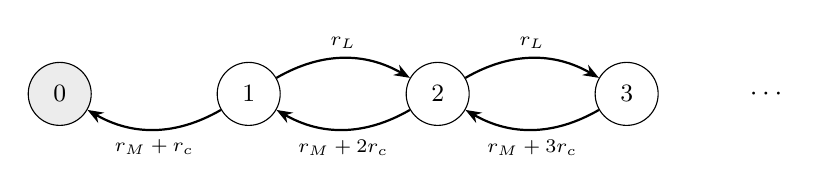
\begin{tikzpicture}[
  st/.style={draw, circle, minimum size=8mm, font=\small},
  arr/.style={-{Stealth[length=2mm]}, thick}]
\node[st, fill=gray!15] (s0) at (0,0) {0};
\node[st] (s1) at (2.4,0) {1};
\node[st] (s2) at (4.8,0) {2};
\node[st] (s3) at (7.2,0) {3};
\node at (9.0,0) {$\cdots$};
\draw[arr, bend left=30] (s2) to node[above, font=\scriptsize]{$r_L$} (s3);
\draw[arr, bend left=30] (s1) to node[above, font=\scriptsize]{$r_L$} (s2);
\draw[arr, bend left=30] (s3) to node[below, font=\scriptsize]{$r_M + 3r_c$} (s2);
\draw[arr, bend left=30] (s2) to node[below, font=\scriptsize]{$r_M + 2r_c$} (s1);
\draw[arr, bend left=30] (s1) to node[below, font=\scriptsize]{$r_M + r_c$} (s0);
\end{tikzpicture}
\end{center}
with birth rate $r_L(s_t/\delta)$ and death rate $r_M + x\,r_c(s_t/\delta)$; reaching state $0$ (shaded) means
the queue has been used up and the price moves, so the count stops there. The authors prove that, up to the first price change,
the two best queues can be replaced by \emph{independent} birth--death processes with these rates. Every
question about the next price move becomes a question about which of two independent counters hits
zero first---the race of Section~\ref{sec:queue-models}, now with exact rates.

\paragraph{Why Laplace transforms.} The time for a birth--death process starting at $x$ to reach zero is
a sum of $x$ independent pieces: the time to go from $x$ to $x-1$, then from $x-1$ to $x-2$, and so on.
Distributions of sums are awkward, but the \emph{Laplace transform} of a waiting time $\tau$,
$\E[\mathrm{e}^{-\varpi \tau}]$ as a function of a variable $\varpi$, turns sums of independent waiting
times into products of their transforms. For birth--death processes each one-step transform has a known
closed form as a continued fraction~\citep{cst2010}, so the transform of the whole first-passage time is a
product of known pieces. Probabilities such as ``queue A empties before queue B'' are then obtained by
numerically inverting a transform built from these products---a computation that takes far less time than
simulating thousands of paths of the book, and gives full distributions rather than only averages.
\inwords{instead of simulating the book many times and counting how often the price went up, the model
writes the answer as a formula in transform space and evaluates it directly. The transform is a
book-keeping device that makes adding independent waiting times as easy as multiplying numbers.}

\subsubsection{Three probabilities a trader needs}

The paper computes three conditional probabilities, each given the current number of orders at the
best bid, $v^b_{1,t}$, and at the best ask, $v^a_{1,t}$, and the spread.

\paragraph{1. Will the next price move be up?} With a one-tick spread, the mid rises next if the ask
queue empties before the bid queue. With a wider spread, a new order can also arrive inside the spread
and move the mid first; the formula adds these arrivals as competing exponential clocks.
Table~\ref{tab:cst-up} compares the model's answer with the empirical frequency in the data. The model
captures the main pattern well---the probability rises with the bid queue and falls with the ask
queue---though it understates how strongly a large ask queue pushes the price down, and some cells
differ noticeably (for example 0.548 against an empirical 0.714 with four orders at the ask and five
at the bid).

\begin{table}[ht]
\centering\footnotesize
\caption{Probability that the next mid move is up, one-tick spread, Sky Perfect Communications:
empirical frequency / Cont--Stoikov--Talreja model (Laplace-transform method)~\citep{cst2010}. Queue sizes
in units of the average limit order.}
\label{tab:cst-up}
\begin{tabular}{lccccc}
\toprule
& \multicolumn{5}{c}{Orders at the best ask, $v^a_{1,t}$} \\
\cmidrule(lr){2-6}
Orders at the best bid, $v^b_{1,t}$ & 1 & 2 & 3 & 4 & 5 \\
\midrule
1 & 0.512 / 0.500 & 0.304 / 0.336 & 0.263 / 0.259 & 0.242 / 0.216 & 0.226 / 0.188 \\
2 & 0.691 / 0.664 & 0.502 / 0.500 & 0.444 / 0.407 & 0.376 / 0.348 & 0.359 / 0.307 \\
3 & 0.757 / 0.741 & 0.601 / 0.593 & 0.533 / 0.500 & 0.472 / 0.437 & 0.409 / 0.391 \\
4 & 0.806 / 0.784 & 0.672 / 0.652 & 0.580 / 0.563 & 0.529 / 0.500 & 0.484 / 0.452 \\
5 & 0.822 / 0.812 & 0.731 / 0.693 & 0.640 / 0.609 & 0.714 / 0.548 & 0.606 / 0.500 \\
\bottomrule
\end{tabular}
\end{table}

\paragraph{2. Will my order at the bid be filled before the price moves?} Suppose an order is placed at
the back of the best bid, so that the bid queue holds $v^b_{1,t}$ orders including our own, and that it
is never cancelled. It is filled when all orders ahead of it
have been removed---by market sells, or by cancellation of the orders ahead---which is a pure-death
process: with $x$ orders in line including our own, the line shortens at rate $r_M + (x-1)\,r_c$, since
our own order is not cancelled. The order is filled before the price moves if this line empties before
the ask queue does. Table~\ref{tab:cst-fill} gives the model's answers. The pattern is the execution
problem of Part~III in numbers: an order alone at the bid, facing five orders at the ask, is filled before
the price moves about 78\% of the time; the last of five orders at the bid, facing one at the ask, about
12\%.
The authors note that their data do not identify individual orders, so these probabilities could not be
checked against data---exactly the gap that order-level data and queue-exact replay fill
(Part~IV).

\begin{table}[ht]
\centering\footnotesize
\caption{Probability that an order placed at the best bid is executed before the mid moves, one-tick
spread, Cont--Stoikov--Talreja model (Laplace-transform method)~\citep{cst2010}.}
\label{tab:cst-fill}
\begin{tabular}{lccccc}
\toprule
& \multicolumn{5}{c}{Orders at the best ask, $v^a_{1,t}$} \\
\cmidrule(lr){2-6}
Orders at the best bid, $v^b_{1,t}$ & 1 & 2 & 3 & 4 & 5 \\
\midrule
1 & 0.497 & 0.641 & 0.709 & 0.749 & 0.776 \\
2 & 0.302 & 0.449 & 0.535 & 0.591 & 0.631 \\
3 & 0.206 & 0.336 & 0.422 & 0.483 & 0.528 \\
4 & 0.152 & 0.263 & 0.344 & 0.404 & 0.452 \\
5 & 0.118 & 0.213 & 0.287 & 0.346 & 0.393 \\
\bottomrule
\end{tabular}
\end{table}

\paragraph{3. Will I ``make the spread''?} A market maker places one order at the best bid and one at
the best ask and earns the spread if both are filled before the price moves. The model computes this
probability too. Its most interesting feature is that it is \emph{not} monotone: for a fixed number of
orders at the ask, the probability first rises and then falls as the bid queue grows. With one order at
the ask, it is about 0.27 with one order at the bid, peaks near 0.31 with two or three, and falls back
to about 0.29 with five. A longer bid queue protects the bid from being exhausted, which helps, but also
makes the bid order wait longer, which hurts; the balance gives an interior optimum.

\subsubsection{What the model reproduces}

Without any tuning for these purposes, the fitted model reproduces several features of the real book:
\begin{itemize}[leftmargin=1.5em,itemsep=2pt]
\item the \textbf{hump-shaped average book}: simulated average depth peaks two ticks from the opposite
  quote, as observed empirically~\citep{bouchaud2002};
\item the \textbf{order of magnitude of volatility}: over the first day of the sample the realised
  volatility was 0.0219 after 370 trades, against $0.0228 \pm 0.0003$ in simulations of the same number
  of trades---computed from order-flow rates alone;
\item the \textbf{one-step behaviour of queues}: the probability that a queue grows at its next change,
  as a function of its size and distance, is close to the empirical frequencies at all five distances.
\end{itemize}

\subsubsection{A trading test, and what it shows}

The authors build a simple strategy on the probability of an up move. When the spread is one tick, there
are at least three orders at the best bid, one at the best ask and at most one at the second ask, buy
with a market order. If one order remained at the second ask, the book now has a two-tick spread, three
or more orders at the bid and one at the ask, and the model gives a 0.62 probability that the next move
is up. Exit with a market sell when the bid rises above the entry price, or when the bid queue falls to
one order (a one-tick loss). In about 30 days of \emph{simulated} trading from the fitted model, the
strategy made 2,376 round trips with an average profit of 0.068 ticks per trade, although fewer than
half of the trades were winners---and without transaction costs.

The test illustrates both the promise and the limits discussed throughout this survey. The decision is
derived from a conditional probability of the book, which is exactly what an execution policy needs.
But it is evaluated inside the model that generated the probability, not on recorded data, and without
costs; a profit of 0.068 ticks per trade must also survive the half spread paid on entry and exit, the
fees, and the latency between seeing the book and the market order arriving. These are the steps of the
chain in Equation~(\ref{eq:chain}) that the model does not cover.

\subsubsection{Limitations and descendants}

The authors are explicit about what the model leaves out. Order arrivals are independent Poisson
streams, so there is no clustering of events and none of the long memory of order flow
(Section~\ref{sec:facts}); orders all have the same size; rates do not change through the day or with
market conditions; and there is no strategic behaviour. Each limitation defines a line of later work:
\begin{itemize}[leftmargin=1.5em,itemsep=2pt]
\item \citet{contlarrard2013,contlarrard2012} reduce the book to the two best queues and obtain closed
  forms and a diffusion limit (Section~\ref{sec:cdl});
\item queue-reactive models let all rates depend on the current queue sizes~\citep{huang2015}, and their
  neural extensions learn that dependence~\citep{deepqr};
\item Hawkes models replace the Poisson streams by self-exciting ones (Section~\ref{sec:hawkes});
\item the micro-price~\citep{stoikov2018} keeps the Markov-chain logic but estimates the transitions
  directly from data rather than from a parametric model;
\item queue-position valuation~\citep{moallemi2017} and fill-probability models~\citep{arroyo2024,kanformer}
  extend the second probability above to individual orders, with adverse selection.
\end{itemize}
Finally, because the Laplace-transform method yields full distributions rather than single
probabilities, it can answer latency questions directly---for example, the probability that the ask
queue empties more than a given delay after the bid queue, which is what matters when an order takes
time to reach the exchange~\citep{cst2010}.

\begin{modelcard}{Cont--Stoikov--Talreja}
\cardrow{What you calibrate}{The limit-order rates $r_L(\bar\ell)$, summarised by $r_0$ and $\Xi$; the
market-order rate $r_M$; the per-order cancellation rates $r_c(\bar\ell)$; the unit of size (the
average limit order).}
\cardrow{How}{Counting: increases, decreases not caused by trades, and market orders at each distance,
divided by trading time (and, for cancellations, by average queue size); a least-squares power-law fit
for $r_L$.}
\cardrow{What you do with it}{Compute, from the current two best queues, the probability that the next
move is up, that a resting order fills before the price moves, and that a market maker earns the
spread---fast and exactly, via Laplace transforms.}
\cardrow{How to picture it}{Two counters racing to zero, each ticking up when an order joins and down
when one is traded or cancelled; the first to hit zero decides the next price move.}
\end{modelcard}

\subsection{The Cont--de Larrard model}
\label{sec:cdl}

\citet{contlarrard2013} give the cleanest closed-form treatment of the race between the two best
queues, and it is worth stating because every term has a direct trading meaning. The model assumes:
\begin{itemize}[leftmargin=1.5em,itemsep=1pt]
\item the spread is always one tick (true over 98\% of the time for the large-tick US stocks they
  study);
\item at each best queue, limit orders arrive at rate $r_L$, market orders at rate $r_M$ and
  cancellations at rate $r_C$, all as independent Poisson streams of unit-size orders, so each queue
  is a random walk that moves up at rate $r_L$ and down at rate $r_M + r_C$
  (in the notation of the bucket picture, $r_{\text{in}} = r_L$ and $r_{\text{out}} = r_M + r_C$);
\item when a queue empties, the price moves one tick and both new best queues are drawn afresh from a
  distribution estimated from the data.
\end{itemize}
Empirically the rates nearly balance: $r_L$ is slightly below $r_M + r_C$ (for example a ratio of
about $0.95$ for Citigroup in their data). Three results follow.

\paragraph{Time to the next price change.} The waiting time has a closed-form distribution in terms
of Bessel functions. Its tail is the important part: when inflow is slightly smaller than outflow,
the probability that no price change has occurred after $u$ seconds decays like $1/u^2$; when they
balance exactly, it decays like $1/u$, so the \emph{expected} waiting time is infinite. Long
quiet periods punctuated by bursts are thus a direct consequence of (nearly) balanced queues, before
any self-excitation is added.

\paragraph{Probability that the next move is up.} In the balanced case the probability depends only
on the two queue sizes, not on the rates---it is the probability that a symmetric two-dimensional
random walk started at the queue sizes hits the ask axis first. In the companion heavy-traffic
analysis~\citep{contlarrard2012}, with uncorrelated queue changes of equal size and intensity on the
two sides, it takes the simple form
\begin{equation}
  \P(\text{next mid move is up} \mid v^b_{1,t}, v^a_{1,t}) =
  \frac{2}{\pi}\arctan\!\left(\frac{v^b_{1,t}}{v^a_{1,t}}\right).
\end{equation}
\inwords{the probability rises from $0$ to $1$ as the bid queue grows relative to the ask queue,
and equals $1/2$ when they are equal. It is the ``thin side breaks first'' rule of
Section~\ref{sec:ofi}, made exact for this model. In Figure~\ref{fig:book}, with 29 lots bid and 14
offered, it gives $(2/\pi)\arctan(29/14) \approx 0.71$.} (The general formula in the paper allows
for correlated queue changes; its printed zero-correlation special case has the two queues
interchanged, and the form above is the one implied by the paper's general expression.)

\paragraph{From queues to volatility.} Over long horizons the price behaves like a random walk whose
volatility, in the balanced case, is proportional to $\delta\sqrt{r_L / \Theta}$, where $\Theta$ is the average
product of the bid and ask queue sizes just after a price change. Volatility rises with order
activity and falls with the depth that reappears after each move---a microstructural explanation of
why thin, busy markets are volatile. Across Dow Jones stocks the authors find ten-minute volatility
roughly proportional to this quantity.

\begin{example}[Why the rates must depend on the state]
\label{ex:fpt}
A best-ask queue holds 200 lots. Averaged over the day, net depletion (executions plus
cancellations minus additions) runs at 40 lots per second, so the first estimate gives
$200/40 = 5$ seconds. Now condition the rate on OFI. When buying pressure is in its top decile, the
net drain is 90 lots per second and $\E[\tau^a] \approx 200/90 \approx 2.2$ s; in the bottom decile
it is 15 lots per second and $\E[\tau^a] \approx 13$ s. The same queue has expected lifetimes six
times apart, depending on what the rest of the market is doing. A model that uses one daily average
rate would be wrong in both directions.
\end{example}

\paragraph{Depletion and adverse selection.} Queue depletion is also where adverse selection
comes from. Consider a resting buy order at the back of the best-bid queue. It is filled only when
everything ahead of it has been traded or cancelled. Because it is last in line, in practice it is
filled mostly by a burst of selling large enough to empty the whole level. And an emptied bid level is, by point~1 above, a downward price move. The
order is therefore filled at the very moment the price is moving against it: the buyer acquires
the lots just as they become cheaper. The fill and the bad price move are not two unlucky events
that happen to coincide; they are the same event.

An order near the \emph{front} of the queue is in a different position. It can be filled by a small
sell order that takes a few lots and leaves the rest of the queue, and the price, where they were.
Such fills carry little information, so front-of-queue orders are less adversely selected. This is
one source of the front--back value difference in \citet{moallemi2017}, whose model splits the value
of an order into a static component---the spread earned minus adverse selection, which increases with
queue position---and a dynamic component, the option value of holding the queue position.

\begin{example}[Filled by the move]
In Figure~\ref{fig:book} we join the best bid at 5000.00 with one lot, behind 29 lots. Suppose a
30-lot sell market order arrives. It takes all 29 lots ahead of us and our lot, and the 5000.00
level is gone: the best bid is now 4999.75 and the mid has fallen from 5000.125 to 5000.00 or below.
We bought at 5000.00 and the market immediately values the contract lower. Had we been first in the
queue, a 2-lot sell would have filled us and left 28 lots and the price untouched.
\end{example}

\begin{modelcard}{Cont--de Larrard}
\cardrow{What you calibrate}{Three rates per best queue, $r_L$, $r_M$, $r_C$, and the distribution of
the new best-queue sizes after a price change (which gives $\Theta$).}
\cardrow{How}{Counting events at the best quotes over a sample, and the empirical distribution of queue
sizes just after each price change.}
\cardrow{What you do with it}{The probability that the next move is up, the distribution of time to
the next price change, and a volatility estimate $\propto \delta\sqrt{r_L/\Theta}$ from order-flow rates
alone.}
\cardrow{How to picture it}{A drunkard's walk in two dimensions, starting at the point (bid size, ask
size): whichever axis the walk hits first decides the price move.}
\end{modelcard}

\subsection{The queue-reactive model}
\label{sec:qr}

\paragraph{The idea.} Cont--Stoikov--Talreja make cancellations proportional to queue size and keep
the other rates fixed. \citet{huang2015} ask the data instead: \emph{how do traders actually behave when
a queue is short, and when it is long?} Their answer is the queue-reactive model, in which the rate of
every kind of event at a queue is an arbitrary function of the current size of that queue (and, in
richer versions, of the neighbouring queues), estimated without assuming a functional form.

\paragraph{State and rates.} The book is described by the queues at the first few price levels on each
side of a reference price $p_{\text{ref}}$ (the mid when the spread is an odd number of ticks; three
levels in the paper, because levels four and five behave like level three). Queue sizes are counted in units of
the average size of events at that level, so a queue of size $x$ holds about $x$ typical orders. In the
basic version each queue is a birth--death process like those of Section~\ref{sec:cst}, but with
size-dependent rates: limit orders arrive at rate $r_L(x)$, and cancellations and market orders remove
units at rates $r_C(x)$ and $r_M(x)$, where $x$ is the current queue size.
\inwords{the model writes down a separate arrival, cancellation and trading rate for each possible queue
size, rather than one rate for all sizes. The data decide how the rates change with size.}

\paragraph{Calibration by counting.} For every event at a queue, record the time since the previous
event at that queue, the event type, and the queue size just before the event. The estimator of the
paper is
\[
  \widehat{r}_L(x) = \frac{\#\{\text{limit orders that arrived while the queue held } x\}}
  {\text{total time the queue spent at size } x},
\]
and likewise for cancellations and market orders. (The paper writes it as the inverse of the mean
waiting time at size $x$, times the fraction of events at size $x$ that were limit orders; the two
forms are algebraically equal.) Bid and ask are pooled by symmetry, and recording restarts whenever
$p_{\text{ref}}$ moves.
\inwords{to learn how fast orders arrive when a queue holds $x$ units, count the arrivals that happened
while it held $x$ units and divide by how long it held $x$ units in total.}

\paragraph{What the data show.} On France Telecom and Alcatel-Lucent (Euronext Paris, 2010--2012, five
levels), the rates are far from those of the simpler models. At the best level, the limit-order rate
is roughly constant in queue size (lower when the queue is empty); the cancellation rate increases
concavely up to about 25 units and then flattens, rather than growing linearly as
Cont--Stoikov--Talreja assume; and the market-order rate \emph{decreases} exponentially with the
available volume---traders hit small queues. The long-run distribution of queue sizes implied by the
fitted rates matches the empirical one closely, and better than a Poisson model with linear
cancellation. Richer versions let the best-level rates depend on the opposite queue: insertion falls
and market orders rise as the opposite queue grows.

\paragraph{Prices.} The full queue-reactive model adds a price. When a best queue empties, the
reference price moves one tick with probability $\pi_{\text{move}}$; and with probability $\pi_{\text{reinit}}$
the whole book is redrawn from its long-run distribution around the new price, which the authors
interpret as the share of price changes driven by outside information. ($\pi_{\text{reinit}} = 1$
recovers the Cont--de Larrard assumption of Section~\ref{sec:cdl}.) The two probabilities are calibrated
to the ten-minute volatility and to the ratio of price continuations to reversals; for France Telecom
$\pi_{\text{move}} = 0.7$ and $\pi_{\text{reinit}} = 0.85$. Order-book dynamics alone, with no outside
information, generate at most about 5 basis points of volatility against 14 observed, and far too much
mean reversion; the authors use this gap to motivate the re-initialisation step, which stands for
information arriving from outside the book.

\paragraph{Uses and descendants.} The model is a simulator of large-tick books that reacts to the
orders a trader adds: the paper uses it to compute execution probabilities and to compare placement
tactics (``fire and forget'' against pegging) for a large order. Its neural extension learns the
dependence of the rates on the book with networks~\citep{deepqr}, and queue-reactive Hawkes models add
self-excitation to the size-dependent rates (Section~\ref{sec:hawkes-variants}).

\begin{modelcard}{Queue-reactive model}
\cardrow{What you calibrate}{The rate functions $r_L(x)$, $r_C(x)$, $r_M(x)$ for each of the first few
levels (and, in richer versions, their dependence on neighbouring queues); the price-move
probabilities $\pi_{\text{move}}$ and $\pi_{\text{reinit}}$.}
\cardrow{How}{Count events by queue size and divide by the time spent at that size; calibrate $\pi_{\text{move}}$
and $\pi_{\text{reinit}}$ to the observed volatility and to the continuation--reversal ratio.}
\cardrow{What you do with it}{Simulate a large-tick book that responds to one's own orders; compute fill
probabilities; compare placement tactics for a large order.}
\cardrow{How to picture it}{A toll booth whose customers and attendant react to the line: when it is
long, more drivers give up and leave; when it is short, cars are served faster.}
\end{modelcard}

\subsection{Decision rules from first-passage times}

Depletion times translate directly into execution decisions.
\begin{description}[leftmargin=1.5em,style=nextline,itemsep=2pt]
\item[Limit or market] If the expected time for a passive order to reach the front and be filled is
  longer than the horizon over which the trader's signal is valid, waiting forfeits the signal;
  crossing the spread is then the better choice despite its cost.
\item[When to cancel] If the estimated depletion time of the side on which an order rests collapses,
  or the race of Section~\ref{sec:cdl} turns against it, the order is about to be filled just
  before an adverse move, and should be cancelled or repriced.
\item[What a queue position is worth] \citet{moallemi2017} split the value of a resting order into a
  \emph{static} part---the spread earned at execution minus the adverse-selection cost, which grows
  with queue position---and a \emph{dynamic} part---the option value of holding a place in the queue
  that advances over time. They find that the front--back difference can be comparable to the
  bid--ask spread for some large-tick US stocks (for example BAC and CSCO), and smaller for others.
\item[Fill probability as survival] The time to fill is a waiting time that, for orders cancelled
  first, is never observed; survival models~\citep{cox1972}, which handle such \emph{censored}
  observations, are the natural statistical tool (Section~\ref{sec:deep-fill}).
\end{description}

Queue-depletion models thus serve execution in two ways: they estimate \emph{when} a resting order
will be filled, and, because a depletion is a price move, they indicate \emph{how informative} the
fill is likely to be. Section~\ref{sec:adverse} develops the second point. Depletion and price
prediction are related but distinct: a depletion model answers \emph{when} a level empties, and says
which way the price goes next only when it is used for the race between the two sides.

% ================================================================
\section{Hawkes processes}
\label{sec:hawkes}
% ================================================================

\paragraph{Works in calm, fails in stress.} The queue models of Section~\ref{sec:queue-models} assume
that orders arrive as independent streams at rates fixed over the sample. In a calm book that is a
reasonable approximation: the Cont--Stoikov--Talreja up-move probabilities of Table~\ref{tab:cst-up}
track the empirical frequencies closely. It breaks down exactly when it matters most. After a large
trade or a news release, rates jump to several times their average for a few seconds, and a model
that uses the day's average rate underestimates how fast queues empty (Example~\ref{ex:fpt}). The
missing ingredient is that events cause events. This section introduces the standard model of that
mechanism.

\subsection{Why not a Poisson process?}

The simplest model of events arriving at random times is the \emph{Poisson
process}~\citep{daley2003}. Divide time into tiny slices and, independently in each slice, let an
event happen with a small fixed probability; in the limit, events arrive at a constant average rate
$\mu$ per second. The number $N(u)$ of events between time $0$ and time $u$---and likewise the
number in any other interval of length $u$---has the distribution
\begin{equation}
  \P\big(N(u) = k\big) = \mathrm{e}^{-\mu u}\, \frac{(\mu u)^k}{k!}, \qquad k = 0, 1, 2, \dots
\end{equation}
\inwords{the chance of seeing exactly $k$ events in $u$ seconds depends only on the average rate
and the length of the interval---not on when the interval starts, and not on anything that happened
before it. The process has no memory: an event now makes the next one neither more nor less
likely. The waiting times between events are independent and exponentially distributed, and the
count in an interval has variance equal to its mean.}

For order-book events these properties fail, in three ways that can be seen in any day of data.
\begin{enumerate}[leftmargin=1.8em,itemsep=2pt]
\item \textbf{Events cluster.} Activity comes in bursts. A large trade is followed by a flurry of
  new orders, cancellations and further trades as other participants react; a news release does the
  same on a larger scale. Between bursts the market can be quiet for long stretches. In a Poisson
  process an event says nothing about the next one, so bursts can only arise by chance, and large
  ones are vanishingly rare.
\item \textbf{Counts vary far more than Poisson allows.} Because of clustering, the number of events
  per second has a variance much larger than its mean, whereas a Poisson count has variance equal to
  its mean~\citep{bacry2015}.
\item \textbf{Event types trigger each other.} A buy market order makes further buy market orders
  more likely, because large orders are split into many small ones and because other traders
  follow; a trade that empties a level triggers cancellations and new limit orders around it. A
  set of independent Poisson processes, one per event type, cannot represent any of this.
\end{enumerate}
A fourth, milder departure is that average activity changes predictably through the day, typically
highest near the open and the close. A Poisson process with a time-varying rate (an
\emph{inhomogeneous} Poisson process) can absorb that pattern, but it still cannot make events
cause other events, which is the defining feature of order flow.

\begin{example}[How rare is a burst under Poisson?]
Suppose events arrive at an average rate of $\mu = 10$ per second. Under a Poisson model the
probability of 30 or more events in a single second is about $2.5 \times 10^{-7}$. Over a 6.5-hour
trading day of 23\,400 seconds, the expected number of such seconds is about $0.006$---roughly one
every 170 trading days. In real order flow, seconds with several times the average activity occur
routinely around large trades and announcements. A model that calls them once-a-year events will
badly underestimate how quickly queues can empty (Section~\ref{sec:queue-models}).
\end{example}

A compact way to remember the difference: a Poisson process is \emph{drizzle}---drops fall
independently at a steady rate, and one drop says nothing about the next. Order flow is a
\emph{storm}---long dry spells broken by downpours, in which each burst of rain makes more rain likely
for a while.

Appendix~\ref{app:pp} gives a self-contained introduction to these ideas: the Poisson, renewal and
Hawkes processes, the conditional intensity, the branching ratio, and the statistics that tell the
three apart on real data, with simulated examples.

The Hawkes process keeps what is convenient about the Poisson process---events at random times,
described by a rate---but lets the rate \emph{rise after each event} and then decay back. It is the
smallest change to the Poisson model that makes events cause events. When every kernel below is
zero, it reduces to independent Poisson processes with rates $\mu_i$.

\subsection{The multivariate model}

Let $N_i(t)$ count events of type $i \in \{1,\dots,K\}$. A linear multivariate Hawkes
process~\citep{hawkes1971} has conditional intensity
\begin{equation}
  \lambda_i(t) = \mu_i + \sum_{j=1}^{K} \int_0^t \phi_{ij}(t-t')\, dN_j(t'),
\end{equation}
with baseline rates $\mu_i$ and non-negative kernels $\phi_{ij}$. Here $\lambda_i(t)$ is the
\emph{intensity}: the expected number of type-$i$ events per second at time $t$. The term
$dN_j(t')$ is nonzero only at the instants $t'$ when a type-$j$ event occurred, so the integral is
simply a sum over past events, and the formula can be read as
$\lambda_i(t) = \mu_i + \sum_j \sum_{\text{past type-}j\text{ events at } t'} \phi_{ij}(t - t')$.
\inwords{the current rate of type-$i$ events is a constant background rate $\mu_i$ plus a ``bump''
for every past event; each bump fades as that event recedes into the past, with a shape set by the
kernel $\phi_{ij}$. Events make further events more likely for a while, the way an earthquake
raises the rate of aftershocks or a viral post triggers reposts.}
The branching matrix $\Gamma_{ij} = \int_0^\infty \phi_{ij}(u)\,du$, the total area under a kernel,
is the expected number of type-$i$ events directly triggered by one type-$j$ event. The process is stationary when the spectral radius
$\rho(\Gamma) < 1$, the largest absolute eigenvalue of $\Gamma$. Then, with
$\mu = (\mu_1, \dots, \mu_K)^\top$ and $I$ the $K \times K$ identity matrix, the stationary mean
intensity vector $\bar\lambda = (\bar\lambda_1, \dots, \bar\lambda_K)^\top$ is
\begin{equation}
  \bar\lambda = (I - \Gamma)^{-1}\mu .
\end{equation}
\inwords{expand the inverse as a geometric series,
$(I-\Gamma)^{-1}\mu = \mu + \Gamma\mu + \Gamma^2\mu + \cdots$. The long-run event rate is the
background events, plus the events they trigger, plus the events \emph{those} trigger, and so on
through every generation. The series converges---the cascade dies out---exactly when
$\rho(\Gamma) < 1$. Readers who know discrete-time linear systems will recognise the condition:
it is the stability condition for $\psi_{k+1} = \Gamma \psi_k + \mu$, a feedback loop whose gain must be
below one.}

\paragraph{A note on notation.} Much of the literature writes the exponential kernel as
$\alpha\mathrm{e}^{-\beta u}$ and the (scalar) branching ratio as $n$. In this survey $\beta$ is
reserved for price impact (Section~\ref{sec:ofi}) and $n$ for event indices, so the decay rate is
written $\omega$ and the branching ratio $\Gamma$ (a $1 \times 1$ branching matrix). With
$\phi(u) = \alpha\mathrm{e}^{-\omega u}$, the branching ratio is $\Gamma = \alpha/\omega$.
Hawkes models have been applied extensively to order flow and price formation~\citep{bacry2015}.

\begin{example}[Endogeneity in two dimensions]
\label{ex:hawkes}
Take buy and sell market orders with $\mu = (1, 1)$ events per second and
\[
  \Gamma = \begin{pmatrix} 0.6 & 0.2 \\ 0.2 & 0.6 \end{pmatrix}.
\]
The eigenvalues are $0.8$ and $0.4$, so $\rho(\Gamma) = 0.8 < 1$. Then
$I - \Gamma = \begin{pmatrix} 0.4 & -0.2 \\ -0.2 & 0.4 \end{pmatrix}$ with determinant $0.12$, and
\[
  \bar\lambda = \frac{1}{0.12}\begin{pmatrix} 0.4 & 0.2 \\ 0.2 & 0.4 \end{pmatrix}
  \begin{pmatrix} 1 \\ 1 \end{pmatrix} = \begin{pmatrix} 5 \\ 5 \end{pmatrix}.
\]
Only one event in five is exogenous. The model says a great deal about clustering and nothing, by
itself, about direction: the two sides are symmetric.
\end{example}

\subsection{Reading the branching matrix}

The branching matrix is the economically interesting output of a fitted Hawkes model. Take two
event types, buy and sell market orders:
\[
  \Gamma = \begin{pmatrix} \Gamma_{BB} & \Gamma_{BS} \\ \Gamma_{SB} & \Gamma_{SS} \end{pmatrix}.
\]
$\Gamma_{BB}$ is the average number of further buy market orders directly triggered by one buy
market order: buys beget buys, for example because a large order is being executed in pieces.
$\Gamma_{SB}$ is the number of sell orders triggered by a buy: a cross effect, for example traders
leaning against a move. A large diagonal relative to the off-diagonal means trends in order flow; a
large off-diagonal means reversal. Asymmetry ($\Gamma_{BS} \ne \Gamma_{SB}$) means one side reacts
more strongly to the other than vice versa. Linear Hawkes models allow only excitation; inhibition
(an event making others \emph{less} likely) requires non-linear extensions. The shape of each kernel
$\phi_{ij}$ says how long an influence lasts: an exponential kernel forgets quickly, a power-law
kernel remembers for a long time.

\paragraph{An analogy: acoustic feedback.} A microphone near a loudspeaker picks up each sound and
plays it again, slightly quieter. If the loop gain is below one, every echo is fainter than the last
and a clap dies away; the closer the gain is to one, the longer the ringing lasts. At a gain of one or
more the echoes grow and the system howls. The branching ratio is that loop gain for order flow: the
average number of events that one event triggers. At $0.8$, a single exogenous event produces on average
$1/(1-0.8) = 5$ events in total, as in Example~\ref{ex:hawkes}; at $0.95$ it produces $20$.

\begin{example}[A chain reaction in the book]
\label{ex:chain}
A stylised sequence at the best ask, all within a few milliseconds:
\begin{center}\small
\begin{tabular}{rl}
\toprule
time & event \\
\midrule
0.0\,ms & a buy market order takes 10 of the 14 lots at the best ask (exogenous) \\
0.3\,ms & two sellers at the best ask cancel, fearing a move up (triggered) \\
0.6\,ms & a buyer joins the best bid, leaning with the flow (triggered) \\
0.9\,ms & a second buy market order takes the remaining lots; the best ask ticks up (triggered) \\
1.2\,ms & new sellers post at the new best ask; buyers follow at the new bid (triggered) \\
\bottomrule
\end{tabular}
\end{center}
One outside event produced four more and a price move. In a Hawkes model each row raises the intensity
of the event types in later rows---entries $\Gamma_{ij}$ for cancellation after trade, trade after
trade, limit order after cancellation---and the fitted kernels say how quickly that influence fades.
\end{example}

\subsection{What Hawkes models are for}

Hawkes models represent clustering, self- and cross-excitation, short-term persistence and the
split between exogenous and endogenous activity. They are valuable for intensity forecasting and
event simulation even when directional alpha is weak. A model can reproduce the temporal
statistics of order flow very well while adding little information about the sign of the next
price move. Hawkes models should therefore be evaluated separately for intensity forecasting,
simulation, price prediction and execution prediction (Table~\ref{tab:three-problems}).

An execution use deserves emphasis. The intensity of aggressive flow on one side is a natural
input to a cancellation decision for a passive order on that side: a spike in sell-market-order
intensity raises the probability that a resting bid is about to be filled at a bad time. This is
an adverse-selection question (Section~\ref{sec:adverse}), not a direction question.

\subsection{From events to prices}

The simplest bridge from event counts to prices treats each mid move as an event. Let $N^{+}(t)$
and $N^{-}(t)$ count the upward and downward mid moves up to time $t$, each of size $\delta_m$. Then
\begin{equation}
  m_t = m_0 + \delta_m\,\big(N^{+}(t) - N^{-}(t)\big).
\end{equation}
\inwords{the price is a running tally of up-ticks minus down-ticks; modelling the two counting
processes models the price.}

Write $\lambda^{+}(t)$ and $\lambda^{-}(t)$ for the intensities of $N^{+}$ and $N^{-}$: the expected
numbers of up and down moves per second. \citet{bacry2013} make the two counts \emph{mutually}
exciting: an up move raises the intensity of down moves and vice versa,
\begin{equation}
  \lambda^{+}(t) = \mu_0 + \int_0^t \alpha\,\mathrm{e}^{-\omega (t-t')}\, dN^{-}(t'), \qquad
  \lambda^{-}(t) = \mu_0 + \int_0^t \alpha\,\mathrm{e}^{-\omega (t-t')}\, dN^{+}(t'),
\end{equation}
\inwords{each down move adds a bump of height $\alpha$ to the up-move rate, and vice versa; the bump
decays at rate $\omega$. The background rate on each side is $\mu_0$.}
The cross-kernel has total weight $\Gamma_{\times} = \alpha/\omega < 1$. This one mechanism
produces the familiar microstructure effects. Measured over short windows, prices look very
volatile because every up-tick tends to be followed by a down-tick (bid--ask bounce); over long
windows that back-and-forth cancels. Writing $\sigma^2(w)$ for the variance of price changes per unit time
measured over windows of length $w$, in units of ticks squared,
\begin{equation}
  \sigma^2(w) = \Lambda\left(\frac{1}{(1+\Gamma_\times)^2} + \Big(1-\frac{1}{(1+\Gamma_\times)^2}\Big)\,\frac{1 - \mathrm{e}^{-(\alpha+\omega) w}}{(\alpha+\omega)\,w}\right),
  \qquad \Lambda = \frac{2\mu_0}{1-\Gamma_{\times}} .
\end{equation}
\inwords{$\Lambda$ is the total rate of price moves. For very short windows the measured variance is
$\Lambda$---every move counts. For long windows it falls to $\Lambda/(1+\Gamma_\times)^2 = 2\mu_0/\big((1-\Gamma_\times)
(1+\Gamma_\times)^2\big)$, because moves that are immediately reversed contribute nothing to the
long-run change. The curve between the two is the ``signature plot'' that practitioners use to choose
a sampling frequency for volatility estimates.} Here cross-excitation \emph{damps} long-run variance.
Self-excitation, by contrast, inflates the variance of event \emph{counts} relative to their mean
rate~\citep{bacry2014}; which effect dominates for prices depends on the structure of the kernel
matrix, not on a single number. The two-dimensional version of the model also reproduces the Epps
effect, the drop in measured correlation between two assets when it is computed over very short
windows~\citep{bacry2013}.

\citet{bacry2014} extend the construction to four kernels linking trades and price changes---trades
exciting trades, prices reverting, trades moving prices, and prices triggering trades---and recover
the concave, relaxing impact of large orders executed in pieces. The same machinery was used early to
study book resilience~\citep{large2007} and to make a zero-intelligence order-book simulator produce
realistic spreads~\citep{munitoke2011}.

\subsection{What fitted Hawkes models find}

\paragraph{Branching ratios.} Estimates of the branching ratio for financial event streams have
been high since the mid-2000s, but the exact value is contested. On E-mini S\&P~500 futures,
\citet{filimonovsornette2012} find it rising from about $0.3$ around 1998--2000 to $0.7$--$0.8$ after
2007, with spikes to $0.9$. \citet{hardimanbercotbouchaud2013}, using power-law kernels, find the
kernel integrating to approximately one---a market at criticality. \citet{filimonovsornette2015}
argue that estimates near one are biased upward by outliers, kernel regularisation, edge effects
and regime shifts---fitting a constant background rate to a period in which the true background
varies; their
re-estimation gives values that later fluctuate between about $0.8$ and $1.1$. On CME NQ market
data, an exponential-kernel fit to packet arrivals gives about $0.80$ (Appendix~\ref{app:pp}).
The defensible summary is that a large majority of events are endogenous, and that the precise
number depends on the kernel family and on how non-stationarity is handled.

\paragraph{Kernel shape and long memory.} Non-parametric estimation~\citep{bacry2016} finds kernels
that decay roughly as power laws with exponent slightly above one (in simulation the method recovers
power laws over six decades of time). In
an eight-dimensional model of DAX and Bund futures (price moves, trades, limit orders and
cancellations, each split by side), trades, limit orders and cancellations mainly excite events of
the same type and side, while price moves on one side mainly excite price moves on the other---mean
reversion. The persistence of order flow is a long-documented fact: the signs of market orders form a
long-memory process with a Hurst exponent of about $0.7$~\citep{lillo2004}, explained mainly by the
splitting of large orders into many small ones~\citep{lillo2005,bouchaud2009}. Power-law Hawkes
kernels are the point-process expression of the same fact.

\subsection{Near-criticality}

When the branching ratio approaches one, appropriately rescaled Hawkes processes converge to
continuous limits. With light-tailed kernels the limit is an integrated Cox--Ingersoll--Ross process,
and the price model of \citet{bacry2013} converges to a Heston stochastic-volatility
model~\citep{jaisson2015}. With heavy-tailed kernels---power laws with tail $\propto u^{-(1+\zeta)}$ with $\zeta \in
(1/2, 1)$---the limit is a \emph{rough} fractional process with Hurst parameter $\zeta -
1/2$~\citep{jaisson2016}, which the authors offer as a microstructural foundation for rough
volatility. Empirically, log-volatility does behave like a fractional process with a Hurst exponent of
order $0.1$---for example $0.125$ for DAX and $0.082$ for Bund futures~\citep{gatheral2018rough}. The lesson for LOB modelling is qualitative: strong endogenous excitation, together with
long memory, generates volatility that is itself random and persistent. It is not that markets
literally sit at a singularity, nor that a single scalar multiplies volatility.

\subsection{State-dependent Hawkes models}

The standard specification lets intensity depend on past events but not on the current book. A
state-dependent form~\citep{morariupatrichi2022} couples the two; one convenient parametrisation is
\begin{equation}
  \tilde\lambda_i(t) = \lambda_i(t)\, \exp\!\left(\vartheta_i^\top X_{t-}\right),
\end{equation}
where $\tilde\lambda_i(t)$ is the state-dependent intensity, $\lambda_i(t)$ the Hawkes intensity
defined above, $\vartheta_i$ a vector of coefficients,
and the state $X_{t-}$ may contain the spread, queue imbalance, depth, volatility or cross-asset variables.
\inwords{take the Hawkes rate and multiply it by a factor that depends on the current book. The
dot product $\vartheta_i^\top X_{t-}$ is a weighted score of the book's features, as in logistic
regression, and the exponential turns any score into a positive multiplier, so the rate can never
go negative.}
The gain is realism; the cost is more parameters and more work to fit them. The relevant question is whether state
dependence provides incremental out-of-sample economic value sufficient to justify that cost.

\begin{modelcard}{State-dependent Hawkes}
\cardrow{What you calibrate}{Everything in the linear Hawkes model, plus the coefficient vector
$\vartheta_i$ that scales each intensity by the current book state.}
\cardrow{How}{Maximum likelihood, as for the linear model, with the book state $X_{t-}$ evaluated just
before each event; more parameters, so more data and regularisation are needed.}
\cardrow{What you do with it}{Intensity forecasts that react to the current spread, imbalance and
depth, for simulation and for timing passive orders.}
\cardrow{How to picture it}{The same aftershock model, with a dial set by the state of the book that
turns every rate up or down.}
\end{modelcard}

\subsection{Fitting Hawkes models in practice}
\label{sec:hawkes-fit}

\paragraph{Maximum likelihood.} The standard method chooses the parameters that make the observed
event times most probable~\citep{ozaki1979}. For a $K$-type process observed on $[0, t_{\text{end}}]$ the
log-likelihood is a sum over types,
\begin{equation}
  \ln \mathrm{Lik} = \sum_{i=1}^{K} \Big( \sum_{n:\ \text{event } n \text{ of type } i} \ln \lambda_i(t_n)
  - \int_0^{t_{\text{end}}} \lambda_i(t')\, dt' \Big),
\end{equation}
\inwords{for every type, reward the model for a high intensity at the moments type-$i$ events
happened, and penalise it for the total number of type-$i$ events it expected.}
Because $\lambda_i$ depends only on $\mu_i$ and on the kernels $\phi_{i1}, \dots, \phi_{iK}$ in row
$i$ of the kernel matrix, the $i$-th term involves only those parameters. As long as no parameter is
shared across rows, the fit splits into $K$ independent problems, one per target type, each with
$1 + K$ kernels' worth of parameters~\citep{wu2019qrhawkes,bacry2015}. For exponential kernels each
term is computed in one pass with a running sum (Appendix~\ref{app:pp-mle}), so the cost grows only
linearly with the number of events~\citep{bacry2015}.

Three practical rules follow. First, parameters have natural bounds---$\mu_i > 0$, jumps
$\alpha_{ij} \ge 0$, decay $\omega > 0$---and the optimiser should enforce them. Second, nothing in the
likelihood forces the fitted $\Gamma$ to satisfy $\rho(\Gamma) < 1$; it must be checked after fitting,
and a fit at or above one read as a sign of non-stationarity or a wrong kernel rather than as a fact
about the market (Appendix~\ref{app:pp-branching}). Third, the likelihood is not convex in the decay
rates, but if the decays are fixed in advance---for example a few exponentials with chosen time
scales---it becomes convex in the background rates and jumps~\citep{wu2019qrhawkes}, so the remaining
fit has a single optimum.

\paragraph{Expectation--maximisation.} Direct maximisation can be unstable because the likelihood is
flat in some directions. The branching structure suggests a different route~\citep{veen2008em}: if we
knew which earlier event triggered each event, or that it was a background event, the parameters would
be simple averages. The EM algorithm alternates between guessing those parents probabilistically and
re-estimating. For one type with kernel $\alpha\mathrm{e}^{-\omega u}$~\citep{lewis2011em}:
\begin{itemize}[leftmargin=1.5em,itemsep=1pt]
\item \emph{E step:} the probability that event $n$ was triggered by earlier event $n'$ is
  $\alpha\mathrm{e}^{-\omega (t_n - t_{n'})}/\lambda(t_n)$, and the probability that it was a background
  event is $\mu/\lambda(t_n)$;
\item \emph{M step:} $\mu$ is the expected number of background events divided by $t_{\text{end}}$; $\Gamma$ is the
  expected number of triggered events divided by the number of events; and $1/\omega$ is the
  probability-weighted average of the parent--child delays $t_n - t_{n'}$; then $\alpha = \Gamma\omega$.
\end{itemize}
\inwords{give each event a fractional family tree, then count: how many events had no parent, how many
children an event has on average, and how long children take to arrive.}

\paragraph{Moments and cumulants.} A second family avoids the likelihood altogether and matches
statistics of the counts. The Wiener--Hopf method estimates kernel shapes from the empirical
second-order statistics of the event streams~\citep{bacrymuzy2016wh} (it underlies the non-parametric
results of~\citet{bacry2016}); the cumulant method NPHC estimates only the integrated kernels---the
branching matrix itself---from second- and third-order integrated cumulants, with no assumption on
kernel shape~\citep{achab2018cumulants}; and method-of-moments calibration with closed-form moments
can be rolled forward through time cheaply~\citep{dafonseca2014}.

\paragraph{The branching ratio from count dispersion.} The simplest moment estimator needs only
counts. Split the data into windows of length $w$, and compute the mean and variance of the number of
events per window; their ratio is the Fano factor $D(w)$ of Appendix~\ref{app:pp-fano}. For a
one-type Hawkes process whose correlations die out on time scales much shorter than $w$,
\citet{hardiman2014branching} show that
\begin{equation}
  \Gamma \approx 1 - \sqrt{1/D(w)} .
\end{equation}
\inwords{self-excitation makes counts burstier than Poisson; the more bursty they are, the closer the
branching ratio is to one. A Poisson stream ($D = 1$) gives $\Gamma = 0$.}
The estimate is biased low for finite windows and exact only as $w$ grows without bound, and because
the sample variance can be zero the authors report medians. Applied to the Fano factors of CME NQ
packet data reported in Appendix~\ref{app:pp-fano}---about 52 at $w = 0.1$\,s and about a thousand at
$w = 60$\,s---the formula gives $\Gamma \approx 0.86$ and $\Gamma \approx 0.97$, against $0.80$ from
the exponential-kernel likelihood fit on the same kind of data. Two cautions make this a teaching
example rather than a measurement. The estimate keeps rising with $w$, the same symptom that a slowly
varying background rate produces~\citep{filimonovsornette2015}. And the same stream with its gaps
shuffled---which destroys all self-excitation but keeps the gap distribution---has $D \approx 17$, for
which the formula would still report $\Gamma \approx 0.76$: dispersion alone does not prove
excitation, because a renewal process with very irregular gaps is also over-dispersed.

\paragraph{Non-stationarity.} A single fit over a long window assumes a constant background rate.
Because activity follows intraday patterns and changes across regimes, such fits overstate
endogeneity~\citep{filimonovsornette2015}. In practice models are fitted over short windows, with a
time-varying background, or with the background modelled explicitly.

\paragraph{Online use.} With exponential kernels the intensity is updated in constant time per event,
which makes Hawkes intensities usable inside a low-latency trading loop. The parameters change more
slowly. One workable scheme, which we describe rather than cite, holds the decay rates fixed during a
session and re-fits the background rates and jumps on a rolling window, starting each fit from the
previous solution; with fixed decays each re-fit is a convex problem. Fully online estimators also
exist: for example, \citet{yang2017online} update non-parametric kernels with projected gradient steps
on a discretised, regularised likelihood, with regret growing only logarithmically in time. Whatever
the scheme, the gradient of the log-likelihood contains the compensator term $-\int \lambda_i$ as well
as the event term, so an update that looks only at the events (``the rate was high when events
happened'') and ignores how many events the model expected will push the intensities up without limit.

\paragraph{Goodness of fit: time rescaling.} A fitted point process can be checked with a classical
transformation. Replace each event time $t_n$ by the expected number of events up to it under the
fitted model, $\int_0^{t_n} \widehat\lambda(t')\,dt'$. If the model is right, the transformed times form
a Poisson process with rate one, so the gaps between them are independent and exponential with mean
one~\citep{ogata1988,brown2002}. A quantile--quantile plot of those gaps against the exponential
distribution, or a Kolmogorov--Smirnov test, shows where the model fails---for example, too few very
short gaps means the model underestimates clustering.

\paragraph{Simulation.} Hawkes paths are generated by \emph{thinning}~\citep{ogata1981}: propose a
candidate event using an upper bound on the current intensity, which is valid because exponential
intensities only decay between events, and accept it with probability equal to the true intensity
divided by the bound. Simulated paths are how a fitted model answers questions that have no closed
form, such as the probability that a queue empties within a given latency.

\paragraph{Software.} The open-source library tick~\citep{bacry2018tick} implements maximum-likelihood
fits with exponential and sum-of-exponential kernels, EM, Wiener--Hopf and cumulant estimators, and
simulation.

\begin{modelcard}{Linear (multivariate) Hawkes}
\cardrow{What you calibrate}{Background rates $\mu_i$; the kernels $\phi_{ij}$---for exponential kernels,
the jumps $\alpha_{ij}$ and decay $\omega$---and hence the branching matrix $\Gamma$.}
\cardrow{How}{Maximum likelihood, split into one problem per target type, with bounded parameters and
a one-pass running sum for exponential kernels; or EM, Wiener--Hopf, cumulant and dispersion estimators.
Fit on short or rolling windows, check $\rho(\Gamma) < 1$ afterwards, and test the fit by time
rescaling.}
\cardrow{What you do with it}{Forecast event intensities and, from them, drift, expected OFI and
depletion times; simulate order flow by thinning; monitor how much activity is endogenous; raise a
cancellation alarm when the aggressive intensity against a resting order spikes.}
\cardrow{How to picture it}{Aftershocks after an earthquake, or acoustic feedback: each event raises
the rate of further events, which fades; the branching ratio is the loop gain.}
\end{modelcard}

\subsection{From intensities to decisions}
\label{sec:hawkes-decisions}

A fitted Hawkes model gives, at every instant, the expected rate of each kind of event. Four
quantities a trader can use follow directly; each is valid only over horizons short enough that the
intensities do not change much, because they decay between events.

\paragraph{Drift.} In the price model of the previous subsection, up and down moves of size
$\delta_m$ arrive at rates $\lambda^+(t)$ and $\lambda^-(t)$, so over a short horizon $H$ the expected
mid change is approximately
\[
  \E[m_{t+H} - m_t] \approx \delta_m\,\big(\lambda^+(t) - \lambda^-(t)\big)\, H .
\]
\inwords{if up moves are currently arriving faster than down moves, the price is expected to drift up,
by one tick per surplus up move.}

\paragraph{Expected order-flow imbalance.} Model six event types at the best quotes: limit orders,
cancellations and market orders on each side, with intensities $\lambda^{L,b}$, $\lambda^{C,b}$,
$\lambda^{M,b}$ (bid queue added to; bid queue cancelled; market \emph{buy}, which takes from the ask)
and $\lambda^{L,a}$, $\lambda^{C,a}$, $\lambda^{M,a}$ (ask queue added to; ask queue cancelled; market
\emph{sell}, which takes from the bid). With $\bar v$ the average event size and the best prices
unchanged, the expected OFI per second is
\[
  \bar v\,\Big( \underbrace{\lambda^{L,b} - \lambda^{C,b} - \lambda^{M,a}}_{\text{net change of the bid queue}}
  \;-\; \underbrace{\big(\lambda^{L,a} - \lambda^{C,a} - \lambda^{M,b}\big)}_{\text{net change of the ask queue}} \Big).
\]
\inwords{the same score as Section~\ref{sec:ofi}, but computed from expected rates instead of observed
events: additions to the bid and removals from the ask count as buying pressure.} It is a forecast of
OFI, which by the regression of Section~\ref{sec:ofi} is a forecast of the price change.

\paragraph{Depletion time.} The bucket picture of Section~\ref{sec:queue-models} needs an inflow and
an outflow. For the best ask, $r_{\text{in}} = \bar v\,\lambda^{L,a}$ and $r_{\text{out}} = \bar
v\,(\lambda^{M,b} + \lambda^{C,a})$, so with the current intensities
\[
  \E[\tau^a] \approx \frac{v^a_{1,t}}{r_{\text{out}} - r_{\text{in}}}, \qquad r_{\text{out}} > r_{\text{in}} .
\]
When this falls below the trader's own latency $T_{\text{lat}}$, a sell order resting in that ask queue
is in danger: if the trader decides to cancel, the level may be swept---filling the order just before
the price moves up---before the cancellation arrives. The
full probability $\P(\tau^a \le T_{\text{lat}})$ has no closed form under a Hawkes model, but can be
estimated by simulating from the current state by thinning.

\paragraph{A branching-ratio monitor.} Re-fitting $\Gamma$ on a rolling window gives a running
measure of how much of current activity is self-generated. A rising value signals a market in which
events are feeding on each other. Two cautions apply. A rise can be produced by a changing background
rate rather than by more excitation~\citep{filimonovsornette2015}; and published estimates differ
widely by instrument, period and method (Section~\ref{sec:hawkes}), so a fixed universal alarm level is
not justified. A threshold should be set from the instrument's own history, and the monitor is a
regime indicator, not a forecast of direction.

\subsection{Variants of the Hawkes model}
\label{sec:hawkes-variants}

The linear model with exponential kernels is a starting point. Each variant below relaxes one of its
assumptions; Table~\ref{tab:hawkes-variants} gives the model card for each.

\paragraph{Sums of exponentials.} Power-law kernels capture long memory but lose the constant-time
update. A power law can be approximated over many decades by a small number of exponentials with
geometrically spaced decay rates---for an exponent of two, about 1.7 exponentials per decade
\citep{bochud2007}---and each exponential keeps its own running sum, so the intensity is still updated
in constant time per event. With the decay rates fixed, the likelihood is convex in the remaining
parameters~\citep{wu2019qrhawkes}.

\paragraph{Nonlinear and inhibitory kernels.} Linear Hawkes kernels can only excite. A nonlinear Hawkes
process passes the sum through a function that keeps the intensity non-negative,
$\lambda_i(t) = h\big(\mu_i + \sum_j \int \phi_{ij}(t-t')\, dN_j(t')\big)$, which allows negative
kernels, that is, events that make others \emph{less} likely; general conditions for a stationary
version were given by~\citet{bremaud1996}. In limit-order-book data, \citet{lu2018} observe inhibition
effects that lead them to nonlinear Hawkes models, and \citet{rambaldi2017marked} find that limit orders
(and cancellations) on one side inhibit the same type on the other side, which they read as a
fair-price effect.

\paragraph{Marks: the size of the event.} A 100-lot trade should excite more than a 1-lot trade, but
the obvious fix---multiplying the kernel by a function of size---is rejected by the data: on Bund and
DAX futures the kernels for different trade sizes have different \emph{shapes}~\citep{rambaldi2017marked}.
The authors instead split events into volume classes and treat each class as its own event type. They
find that large trades excite limit orders on the opposite side, and that large orders are more
exogenous than small ones.

\paragraph{Regimes.} In a Markov-modulated Hawkes process a hidden state switches among a few regimes,
each with its own background rate and decay, and the parameters are fitted by EM~\citep{wang2012mmhp}.
It was developed for earthquake sequences (main shocks, aftershocks, quiescence); the analogue for markets
is a model whose quiet and busy regimes have different parameters, rather than one set of parameters
averaged over both.

\paragraph{Quadratic Hawkes and the Zumbach effect.} Volatility has a time asymmetry: past volatility
measured over long horizons predicts future short-horizon volatility better than the reverse---the
\emph{Zumbach effect}~\citep{zumbach2009}. A Hawkes intensity that depends only on past event counts
cannot produce it. The quadratic Hawkes model of~\citet{blanc2017qhawkes} adds a term in the
\emph{square} of a moving average of past signed price changes, so that a sequence of moves in the same
direction raises activity more than the same number of moves that cancel out. Calibrated on five-minute
bins of 133 NYSE stocks over 2000--2009, it reproduces the time asymmetry, and it generates long memory
in volatility without requiring the process to be critical.

\paragraph{Queue-reactive Hawkes.} \citet{wu2019qrhawkes} combine the two ideas of this part: the
background rates depend on the current queue size, as in Section~\ref{sec:qr}, and events excite each
other through sum-of-exponential kernels. On Bund and DAX futures the Hawkes term greatly improves the
pure queue-reactive model, both in the distribution of times between events and in the distribution of
queue sizes; market-order and price-change rates are mainly functions of the volume imbalance, while
limit and cancellation rates are not.

\paragraph{Cross-asset Hawkes.} Events in one instrument can excite events in another; this is the
point-process form of lead--lag, discussed in Section~\ref{sec:cross}.

\begin{table}[ht]
\centering\footnotesize
\caption{Model cards for the Hawkes variants.}
\label{tab:hawkes-variants}
\setlength{\tabcolsep}{3pt}
\begin{tabularx}{\linewidth}{>{\raggedright\arraybackslash}p{0.14\linewidth}*{4}{>{\raggedright\arraybackslash}X}}
\toprule
Variant & What you calibrate & How & What you do with it & How to picture it \\
\midrule
Sum of exponentials & jumps per (pair of types, decay); decays fixed on a geometric grid & convex likelihood once decays are fixed & long memory with constant-time updates, in software or hardware & a power law drawn with a few rulers of different lengths \\
Nonlinear / inhibitory & signed kernels; the link function & maximum likelihood (poorly convex) & represent events that discourage others & a thermostat as well as an amplifier \\
Marked (volume classes) & one set of kernels per size class & as for a multivariate model, one type per class & let large trades matter more, with their own time profile & a big stone makes bigger, longer ripples \\
Markov-modulated & per-regime background and decay; switching rates & EM over hidden regimes & separate quiet and busy regimes & weather that switches between drizzle and storm \\
Quadratic (Zumbach) & self-excitation kernel; return-feedback kernel & on binned returns (GMM, then likelihood) & volatility forecasts with the right time asymmetry & a trend, not just activity, wakes the market up \\
Queue-reactive Hawkes & size-dependent background; excitation kernels & maximum likelihood with fixed decays & simulate queues with realistic clustering & the toll booth of Section~\ref{sec:qr}, with rush hours \\
\bottomrule
\end{tabularx}
\end{table}

\subsection{Neural point processes}
\label{sec:npp}

\paragraph{Where we are.} Everything so far in this section has the same structure: the rate of
type-$i$ events is a background rate plus a sum of bumps, one per past event, each with a fixed shape
$\phi_{ij}$. The variants of Section~\ref{sec:hawkes-variants} change one ingredient at a time---the
shape of the bump, its sign, its dependence on size or on the queue. A neural point process changes
all of them at once: it keeps the idea of an intensity, but lets a neural network compute it from the
history. This subsection explains what that means, step by step.

\paragraph{What the Hawkes formula cannot say.} Three limitations of the linear Hawkes model motivate
the step.
\begin{enumerate}[leftmargin=1.8em,itemsep=2pt]
\item \textbf{Effects only add.} Each past event contributes its own bump, independently of the
  others. In the chain reaction of Example~\ref{ex:chain}, a trade followed by two cancellations at the
  same level is far more alarming than either alone: together they say the level is about to go.
  A sum of separate bumps cannot express ``A \emph{and then} B matters more than A plus B''.
\item \textbf{The shape is fixed in advance.} The analyst chooses exponential, power law, or a sum of
  exponentials, and the data only set the parameters.
\item \textbf{The rate can only jump up and then decay.} Between events, a linear Hawkes intensity
  with positive kernels can only fall. Real flow can do the opposite: after a sweep, new limit orders
  may arrive slowly at first and then faster as participants re-quote.
\end{enumerate}

\paragraph{The recipe.} Every neural point process has three parts.
\begin{description}[leftmargin=1.5em,style=nextline,itemsep=2pt]
\item[1. Describe each event as a vector] Event $n$ is turned into a vector of numbers (an
  embedding) built from its type, the time since the previous event $t_n - t_{n-1}$, and any marks
  such as size or side.
\item[2. Summarise the history] A sequence model reads the embeddings of events $1, \dots, n$ in order
  and produces a \emph{history vector} $\mathbf{z}^{\text{hist}}(t)$ that summarises everything that
  happened before time $t$. This is the role played in a Hawkes model by the running sums of decaying
  bumps.
\item[3. Turn the summary into intensities] For each event type $i$, the intensity is
\end{description}
\begin{equation}
  \lambda_i(t) = \operatorname{softplus}\!\big(\langle \mathbf{o}_i, \mathbf{z}^{\text{hist}}(t)\rangle\big),
  \qquad \operatorname{softplus}(y) = \ln\big(1 + \mathrm{e}^{y}\big),
\end{equation}
where $\mathbf{o}_i$ is a vector of learned output weights for type $i$ and $y$ stands for any real
number.
\inwords{score the current history with a weighted sum, one set of weights per event type, and pass
the score through the softplus, a smooth function that is always positive and close to the score
itself when the score is large. Rates must be positive; softplus guarantees it, as the exponential
did in the state-dependent model.}
A linear Hawkes model is the special case in which the ``summary'' is the vector of running sums
$\sum \phi_{ij}(t - t_{n'})$ and the output step simply adds them to $\mu_i$. A neural model replaces
the hand-written summary with a learned one.

\paragraph{Training: the same likelihood as Hawkes.} The parameters---the network weights and the
output weights $\mathbf{o}_i$---are fitted by maximising exactly the log-likelihood of
Section~\ref{sec:hawkes-fit}: reward high intensity at the times events happened, penalise the
total expected number of events $\int \lambda_i$. Gradient descent replaces the specialised
optimisers, because the network has many parameters. One new difficulty appears. For an exponential
kernel the integral $\int \lambda_i$ has a closed form; for a neural intensity it usually does not, and
is estimated numerically---commonly by evaluating the intensity at randomly sampled times between
events and averaging (Monte Carlo integration). Two lines of work remove this approximation:
\citet{omi2019} model the \emph{integral} of the intensity with a network constrained to be increasing,
and obtain the intensity as its derivative, so the likelihood is exact; \citet{shchur2020ifl} skip the
intensity altogether and model the probability distribution of the time to the next event directly,
for example as a mixture of simple distributions, which also makes sampling the next event exact.

\paragraph{Three ways to summarise the history.} The models in the literature differ mainly in step 2.
\begin{description}[leftmargin=1.5em,style=nextline,itemsep=2pt]
\item[Recurrent networks] An early and widely cited model, RMTPP~\citep{du2016rmtpp}, updates a recurrent
  network's state at each event and lets the intensity change between events through a fixed function
  of the elapsed time. The \emph{neural Hawkes process}~\citep{mei2017} makes the recurrent state itself
  evolve in continuous time: each memory cell of an LSTM decays exponentially between events towards a
  target value set at the last event. Because the target can be above or below the current value, the
  intensity can rise or fall between events, and one event can make another \emph{less} likely---the
  inhibition that linear Hawkes cannot represent.
\item[Attention] The Transformer Hawkes process~\citep{zuo2020thp} and the self-attentive Hawkes
  process~\citep{zhang2020sahp} let each event attend to all earlier events, as in the
  queries--keys--values box of Section~\ref{sec:deep}, with the time gaps encoded into the
  embeddings. The attention weights play the part of the kernel: they say how much each past event
  matters now, but are computed from the content of the events rather than fixed in advance.
  \citeauthor{zhang2020sahp} argue that the attention weights also give an interpretable measure of
  influence between event types.
\item[State-space models] The Mamba Hawkes process~\citep{gao2024mhp} summarises the history with a
  selective state-space model (Section~\ref{sec:deep}), which processes long sequences in time linear in
  their length.
\end{description}
\citet{shchur2021} survey the family and its design choices.

\begin{example}[What a learned summary can add]
Take the chain reaction of Example~\ref{ex:chain}. A two-type Hawkes model of trades and ask
cancellations gives the intensity of a further buy market order as background plus one bump for the
trade and one for each cancellation, whatever their order. A neural model reads the sequence ``buy
trade, cancel, cancel'' as a whole. If, in the training data, that particular pattern was usually
followed within a millisecond by a sweep of the level, the model can raise the intensity of buy market
orders far more than the sum of the separate bumps would, and leave it unchanged after the same three
events in a different order. Whether it learns this depends entirely on whether the pattern is
frequent enough in the data; the flexibility is useless without the examples.
\end{example}

\paragraph{Applications to order books.} The Transformer Hawkes process and the Mamba Hawkes process
both report results on a data set of financial transactions (buy and sell events of a stock over a
day), among other benchmarks~\citep{zuo2020thp,gao2024mhp}. Models built specifically for the book go
further. \citet{shi2022sdpnhp} compute a separate intensity for each order-book event type with
parallel continuous-time LSTMs and add an interaction between events and the state of the book; on
five days of LOBSTER data for three US stocks it outperforms both classical and neural point-process
baselines in likelihood, timing and event-type accuracy, and the authors note that their simulator
settings remain simple. \citet{lalor2025nhp} drive a twelve-event-type order-book simulator with an
LSTM-based neural Hawkes process and use it as the training environment for a reinforcement-learning
market maker.

\paragraph{What is lost.} The flexibility has three costs, and each matters in this survey's setting.
\begin{itemize}[leftmargin=1.5em,itemsep=2pt]
\item \textbf{Interpretability.} A linear Hawkes fit returns a branching matrix whose entries have a
  meaning (Section~\ref{sec:hawkes}) and a branching ratio that can be monitored. A neural model returns
  weights; quantities such as the fraction of endogenous events have no direct equivalent.
\item \textbf{Speed.} An exponential Hawkes intensity is updated with a few multiplications per event.
  A neural intensity needs a forward pass of a network per event, and more if the intensity is needed
  between events---a cost that matters inside a trading loop (Section~\ref{sec:hardware}).
\item \textbf{Guarantees.} The stability condition $\rho(\Gamma) < 1$ has no simple analogue, so a
  simulated neural model can drift into regimes never seen in training.
\end{itemize}
The evaluation follows Principle~3. The baseline is a multivariate Hawkes model, ideally with
sum-of-exponential kernels, fitted to the same events; the comparison is the held-out log-likelihood per
event, the time-rescaling test of Section~\ref{sec:hawkes-fit} (which applies to any model that outputs
an intensity), and, for a trading use, the economic value of the forecasts. A neural point process
earns its place when it improves these by more than its cost in speed and interpretability.

\begin{modelcard}{Neural point processes}
\cardrow{What you calibrate}{The embedding of events, the weights of the sequence model that summarises
the history (recurrent, continuous-time recurrent, attention or state-space), and the output weights
$\mathbf{o}_i$ that turn the summary into an intensity for each event type.}
\cardrow{How}{Gradient descent on the point-process log-likelihood, with the integral of the intensity
estimated by Monte Carlo, or made exact by modelling the integral or the next-gap distribution
directly. Compare on held-out likelihood and by time rescaling against a multivariate Hawkes baseline.}
\cardrow{What you do with it}{Predict the type and time of the next event; simulate order flow,
including as a training environment for execution or market-making agents; capture interactions
between events that additive kernels miss.}
\cardrow{How to picture it}{A Hawkes model whose bumps are drawn by a network that has read the whole
history in order, instead of by a fixed formula: it can notice that ``trade, cancel, cancel'' means
more than the three events separately.}
\end{modelcard}

% ================================================================
\section{Deep learning for limit order books}
\label{sec:deep}
% ================================================================

Deep learning entered LOB research around 2017 and now dominates the volume of published work. This
section describes what the main families of models actually do, what the large benchmark studies
have found when the models are re-tested, and which design choices matter. Readers new to the
architectures will find short definitions of convolutional, recurrent and attention-based networks
in the glossary (Appendix~\ref{app:glossary}) and textbook treatments in~\citet{goodfellow2016}.

\subsection{Problem formulations}

Most deep LOB papers solve one of six problems:
\begin{description}[leftmargin=1.5em,style=nextline,itemsep=2pt]
\item[Direction classification] predict whether the mid will be up, down or stationary after a horizon $H$
  measured in events or seconds. Labels are usually built by comparing a smoothed future mid with the current one
  against a threshold; the choice of smoothing and threshold changes the problem, and a recent paper
  shows that coupling the smoothing window to the horizon biases the labels~\citep{berti2025tlob}.
\item[Multi-horizon forecasting] predict returns, or their direction, over several horizons at
  once---an ``alpha term structure''~\citep{kolm2023,zhangzohren2021}.
\item[Next-event prediction] predict the type, side, price and size of the next message---the
  natural task for message-level and point-process models~\citep{linna2025lobert}.
\item[Full-book forecasting] predict the whole future book, prices and volumes at several
  levels~\citep{arxiv240902277}.
\item[Fill-time estimation] predict the distribution of the time until a resting order is filled
  (Section~\ref{sec:deep-fill}).
\item[Generation] produce synthetic message streams or book snapshots (Section~\ref{sec:deep-gen}).
\end{description}

\paragraph{The benchmark data set.} A large share of the literature reports results on FI-2010
\citep{ntakaris2018}: five stocks from the Helsinki exchange over ten trading days in June 2010,
about 4.5 million messages, ten levels, already normalised and downsampled into blocks of ten
events. It made comparison possible, and it also made overfitting easy. The DeepLOB authors
themselves describe it as ``far too short, downsampled and taken from a less liquid
market''~\citep{zhang2019}. Results on it should be read with the comparability fields of
Section~\ref{sec:comparable} in mind.

\subsection{Convolutional and recurrent models}

\paragraph{First models.} \citet{tsantekidis2017} applied a convolutional network to sequences of
book snapshots, treating the book like an image whose two axes are time and price level. A
companion paper used an LSTM with 40 hidden units on the last 100 snapshots, reporting F1 scores
of about 61--66\% on FI-2010 against 48--56\% for a multilayer perceptron~\citep{tsantekidis2017lstm}.
\citet{dixon2018} applied a recurrent network to E-mini S\&P~500 Level-2 data to classify the next
price flip.

\paragraph{DeepLOB.} \citet{zhang2019} combined the two ideas and became the most widely used
reference architecture. Its input is the last 100 snapshots of ten levels (40 numbers each:
price and size for bid and ask at each level). Small convolutions first combine price with size at
each level, then bid with ask, then levels with each other; an Inception module applies parallel
convolutions over several time scales; a 64-unit LSTM summarises the sequence; and a softmax outputs
probabilities for down, stationary and up. On a year of London Stock Exchange data for five stocks it
reports F1 of about 70\%, 63\% and 61\% at horizons of 20, 50 and 100 events, with similar numbers on
five stocks not seen in training---evidence that it learns features that transfer. Its trading
simulation, as the authors state, uses mid-prices without transaction costs and is ``not \ldots a fully
developed, stand-alone trading strategy''.

\paragraph{Learning across many stocks.} \citet{sirignano2019dl} introduced a ``spatial'' network that
exploits the ordering of price levels to use information deep in the book with few parameters,
trained on 489 US stocks over twenty months on a GPU cluster; it outperforms logistic regression and a
standard network, especially in the tails of the distribution. \citet{sirignano2019} train a single
model on many stocks and find that it outperforms stock-specific models, which they interpret as
evidence of universal features of price formation.

\paragraph{Lighter models and normalisation.} Not every gain needs more capacity. The temporal
attention-augmented bilinear network (TABL) acts separately on the feature and time axes of the input
matrix and reaches competitive FI-2010 results with about $10^4$ parameters~\citep{tran2019tabl}.
Deep adaptive input normalisation (DAIN) learns how to normalise each input
feature~\citep{passalis2020dain}; on FI-2010 it raises the macro-F1 of a simple MLP from about 55\%
with standard z-scoring to about 68\%. Because the statistics of LOB data drift, how inputs are
normalised is a modelling decision in its own right.

\begin{modelcard}{Convolutional and recurrent models (DeepLOB family)}
\cardrow{What you calibrate}{The network weights (from about $10^4$ to $10^5$ parameters for TABL and
DeepLOB), and before that the input normalisation, the label threshold and the horizon.}
\cardrow{How}{Supervised training with a cross-entropy loss on labelled windows of snapshots
(down/stationary/up), with chronological train, validation and test splits.}
\cardrow{What you do with it}{Short-horizon direction probabilities, used as a signal or as one input
to an execution decision.}
\cardrow{How to picture it}{The book as an image---time across, price levels down---scanned by small
filters that find local patterns, followed by a memory that reads the patterns in order.}
\end{modelcard}

\subsection{Attention and spatial-temporal models}

\paragraph{Attention.} An attention layer lets each element of a sequence form a weighted average of
all the others, with weights computed from the data~\citep{vaswani2017}. Applied to LOBs, the
sequence can run along time, along price levels, or along assets. A model that attends along more
than one of these axes is called \emph{spatial-temporal}: ``space'' is the price ladder (and, in
multi-asset models, the set of instruments), ``time'' is the sequence of snapshots or events.

\begin{tcolorbox}[breakable, enhanced, colback=black!3, colframe=black!45, boxrule=0.5pt, arc=1.5pt,
  fonttitle=\bfseries\small, title={Queries, keys and values on an order book}, fontupper=\small]
Each event $n$ is first turned into a vector of numbers (its embedding). Three learned matrices turn
that vector into a \emph{query} $\mathbf{z}^{\text{qry}}_n$ (``what am I looking for?''), a \emph{key}
$\mathbf{z}^{\text{key}}_n$ (``what do I contain?'') and a \emph{value} $\mathbf{z}^{\text{val}}_n$
(``what do I pass on?''), each of dimension $\dim_{\text{emb}}$. Event $n$ attends to earlier event
$n'$ with weight
\[
  \mathrm{att}_{n n'} = \frac{\exp\big(\langle \mathbf{z}^{\text{qry}}_n, \mathbf{z}^{\text{key}}_{n'}\rangle/\sqrt{\dim_{\text{emb}}}\big)}
  {\sum_{n'' \le n} \exp\big(\langle \mathbf{z}^{\text{qry}}_n, \mathbf{z}^{\text{key}}_{n''}\rangle/\sqrt{\dim_{\text{emb}}}\big)},
  \qquad \text{output}_n = \sum_{n' \le n} \mathrm{att}_{n n'}\, \mathbf{z}^{\text{val}}_{n'} .
\]
\inwords{each event scores every earlier event by how well its key matches the query, turns the scores
into weights that sum to one (the softmax), and takes the weighted average of their values.}

\emph{A stylised sweep.} The current event is a buy market order that empties the best ask. If training
has taught the model that sweeps matter when sellers have been leaving, the sweep's query matches the
keys of the ask cancellations in the last few milliseconds, which receive most of the weight; the bid
limit orders and the quiet stretch before them receive little. The output is, in effect, a summary
``sellers were pulling before this sweep''---the chain reaction of Example~\ref{ex:chain}, read off by
a learned look-up rather than a fixed kernel.
\end{tcolorbox}

\paragraph{TransLOB.} \citet{wallbridge2020} combined five dilated causal convolutions with two
Transformer blocks using masked (causal) self-attention, and reported FI-2010 F1 of 81--92\% across
horizons. An independent re-implementation obtained 59\% on the same data~\citep{prata2024}---the
largest gap between claimed and reproduced performance among the fifteen models tested there, and a
reminder that results on one small data set are fragile.

\paragraph{Axial and dual attention.} Axial-LOB~\citep{kisiel2022axial} applies gated attention
separately along the time and feature axes, keeping the parameter count below $10^4$. TLOB
\citep{berti2025tlob} alternates temporal self-attention (across snapshots) with spatial
self-attention (across the features of a snapshot); its companion MLPLOB replaces attention by
multilayer perceptrons that mix along the two axes, and matches TLOB on several data sets. Three
observations from TLOB are instructive. Performance on Nasdaq and Bitcoin data falls steeply with the
horizon---for INTC, F1 drops from about 80\% at 10 events to about 50\% at 100---whereas on FI-2010 it
\emph{rises} with the horizon, a sign of the data set's peculiarities. Predictability on the same stock
declined between 2012 and 2015. And when the label threshold is set to the average spread, so that
only moves large enough to pay for crossing count, F1 drops to 31--41\% (TSLA, horizons of 50 to 200
events). The authors conclude that the
methods ``are not sufficiently mature for practical deployment''.

\paragraph{Patches, full books and many assets.} LiT~\citep{lit2025} cuts the book into structured
patches---one side of the book over a short time window---as vision Transformers do with images, and
applies it to Binance cryptocurrency data. \citet{arxiv240902277} forecast the entire five-level book
with a sequence-to-sequence Transformer and a loss that penalises forecasts violating the ordering of
prices; on one day of data a linear model is slightly better on the overall forecasting error and
on volumes, but worse on the mid-price and much worse at respecting the ordering of prices. OF-MATNet
\citep{ofmatnet} feeds multi-level order-flow imbalance from many Nasdaq assets into a Transformer
that attends along time, assets and levels, choosing peer assets by rolling Granger-causality tests,
and reports improvements in out-of-sample $R^2$ in over 90\% of cases on 110 assets. HLOB
\citep{briola2025hlob} builds a graph over volume levels and processes it with a homological
convolutional network.

\paragraph{Multi-horizon models and training hardware.} \citet{zhangzohren2021} attach a
sequence-to-sequence decoder with attention to the DeepLOB encoder to produce forecasts at several
horizons at once, and report that training on Graphcore intelligence processing units took about
15\% of the wall-clock time of a GPU.

\begin{modelcard}{Attention and spatial-temporal Transformers}
\cardrow{What you calibrate}{The query, key and value matrices of every attention layer, the feed-forward
weights, and the choice of axes (time, levels, assets) along which to attend.}
\cardrow{How}{Supervised training as for the convolutional models; reproduction studies show that the
result depends heavily on the data set and labelling, so re-testing on new data is part of
calibration.}
\cardrow{What you do with it}{Direction and multi-horizon forecasts, full-book forecasts, and
multi-asset models that choose which peers to read.}
\cardrow{How to picture it}{Every event asks a question of every earlier event and listens most to the
ones whose answers match.}
\end{modelcard}

\subsection{State-space models}

Structured state-space sequence models such as S4~\citep{gu2022s4} and Mamba~\citep{gu2024mamba}
process long sequences with a learned linear recurrence---the same mathematical object as the
classical state-space model of control theory~\citep{kalman1960}---computed efficiently in parallel.
They are attractive for event streams, which are long and irregular. Apart from a hardware-aware design for cryptocurrency tick data~\citep{popov2026ssm}, we could not
identify a widely cited state-space model for LOB forecasting at the time of writing; this is an open
direction rather than an established result (Section~\ref{sec:agenda}).

\begin{modelcard}{State-space sequence models}
\cardrow{What you calibrate}{The matrices of a learned linear recurrence and, for selective models such
as Mamba, the functions that set its step size from the input.}
\cardrow{How}{Supervised training by gradient descent, with the recurrence computed in parallel during
training.}
\cardrow{What you do with it}{Long-context forecasts on long, irregular event streams; for LOB data this
is an open direction rather than an established result.}
\cardrow{How to picture it}{A Kalman-style running state, updated at every event, whose rate of
forgetting is learned.}
\end{modelcard}

\subsection{What the large benchmark studies show}
\label{sec:benchmarks-dl}

Individual model papers report results on their own terms. Two studies re-test many models under
common conditions, and two more vary the input or the evaluation while holding the model fixed; their
findings are more informative than any single paper.

\paragraph{LOBCAST.} \citet{prata2024} re-implemented fifteen published models and tested them on
FI-2010 and on new Nasdaq data from 2021 and 2022. Their headline is that ``all models exhibit a
significant performance drop when exposed to new data'': F1 on the new data lies between 48\% and 61\%
for every model. The best model on the new data, BiNCTABL, loses about a fifth of its FI-2010
score. Five of the six best models use attention. A simple MLP ranks near the bottom but degrades the
least. Parameter counts range from about $10^4$ to $10^7$, with no clear relation between size and
degradation. A trading simulation shows that profitability ``is far from guaranteed''.

\paragraph{Simple models on the same inputs.} \citet{briola2020} compare a random classifier,
logistic regression, an MLP, LSTMs and a CNN--LSTM on identical inputs for one large-tick stock. The
MLP matches or exceeds the CNN--LSTM at all three horizons, while logistic regression is clearly worse.
Linear models are not generally competitive with deep ones on raw book inputs; small non-linear
models often are.

\paragraph{Representation.} \citet{lucchese2024} hold the DeepLOB architecture fixed and change only
the input, on ten Nasdaq stocks. Models fed order-flow inputs or a new volume-on-a-price-grid
representation ``considerably'' outperform those fed the raw level-by-level book, and predictability
is detected up to about 50 order-book events ahead at the 99\% confidence level, using model
confidence sets~\citep{hansen2011mcs} to compare models. The authors stress that mid-to-mid returns
``are not tradable in practice''. \citet{kolm2023}, on 115 Nasdaq stocks, find that networks
trained on order flow ``significantly outperform most models trained directly on order books'', and
that the effective horizon of stock-specific forecasts is about two average price changes. In a later
practitioner-oriented account, as reported in coverage of the authors' 2026 award, very deep models
``don't really help'' for this task, and careful time-stamping and stationary transformations of inputs
mattered more~\citep{kolm_westray}. \citet{wu2021robust} show that level-based inputs are fragile:
adding orders in empty price ticks drops DeepLOB's accuracy from about 77\% to about 51\%, and they
propose representations on a fixed price grid as an alternative.

\paragraph{From forecasts to trades.} \citet{briola2024} retrain DeepLOB on fifteen Nasdaq stocks
grouped by tick size and introduce a transaction-level score,
\begin{equation}
  \mathrm{TO} = \frac{N_{\text{correct}}}{N_{\text{possible}} + N_{\text{predicted}} - N_{\text{correct}}},
\end{equation}
where $N_{\text{possible}}$ counts the round-trip trades (open, then close) that the true price path
would have allowed, $N_{\text{predicted}}$ those the forecasts would have triggered, and
$N_{\text{correct}}$ those in both sets.
\inwords{$\mathrm{TO}$, which its authors call $p_T$, is the overlap between the trades the model would make and the trades that were
actually there to be made, as a fraction of their union---a score of 1 means the model traded exactly
the available opportunities, 0 means no overlap.} The values are sobering: between about 0.01 and 0.19
across stocks and horizons, and close to zero for small-tick stocks once a confidence threshold is
applied, even where F1 is high. Predictability, by both F1-type and transaction-level measures, is
higher for large-tick stocks---those whose average spread is below about 1.5 ticks---than for
small-tick stocks, whose spread exceeds about 3 ticks. The authors conclude that ``high forecasting
power does not necessarily correspond to actionable trading signals''.

\begin{table}[ht]
\centering\footnotesize
\caption{Selected deep LOB models. F1 values are as reported by the authors on the data stated and
are not comparable across rows (Section~\ref{sec:comparable}).}
\label{tab:deep-models}
\setlength{\tabcolsep}{2pt}
\begin{tabularx}{\linewidth}{l*{4}{>{\raggedright\arraybackslash}X}}
\toprule
Model & Architecture & Data & Reported result & Independent re-test \\
\midrule
CNN~\citep{tsantekidis2017} & convolutions over time $\times$ levels & FI-2010 & F1 55--59\% & -- \\
LSTM~\citep{tsantekidis2017lstm} & 40-unit LSTM & FI-2010 & F1 61--66\% & -- \\
DeepLOB~\citep{zhang2019} & CNN + Inception + LSTM, $\sim$60k params & LSE, 5 stocks, 2017 & F1 61--70\% & re-trained on Nasdaq~\citep{briola2024}: $p_T$ 0.01--0.19 \\
TABL~\citep{tran2019tabl} & bilinear + temporal attention, $\sim$10k params & FI-2010 & F1 73--74\% & 70\% on FI-2010, 60\% on 2021 data~\citep{prata2024} \\
TransLOB~\citep{wallbridge2020} & dilated causal CNN + Transformer & FI-2010 & F1 81--92\% & 59\% on FI-2010~\citep{prata2024} \\
Axial-LOB~\citep{kisiel2022axial} & axial attention, $<$10k params & FI-2010 & F1 76--86\% & 73\% on FI-2010~\citep{prata2024} \\
TLOB~\citep{berti2025tlob} & dual spatial/temporal attention & FI-2010, Nasdaq, BTC & F1 to 93\% (FI-2010); 50--80\% (INTC) & -- \\
LiT~\citep{lit2025} & structured patches + Transformer & Binance, 2024 & F1 59--66\% & -- \\
OF-MATNet~\citep{ofmatnet} & multi-asset, multi-axis attention on OFI & 110 Nasdaq assets & $R^2$ gains in $>$90\% of cases & -- \\
\bottomrule
\end{tabularx}
\end{table}

\subsection{Representation versus architecture}

The benchmark evidence suggests that the choice and treatment of inputs can matter as much as the
network---a synthesis across studies, since none compares both systematically. Four decisions should be made, and reported, before capacity is increased.
\begin{description}[leftmargin=1.5em,style=nextline,itemsep=2pt]
\item[Representation] raw levels, order flow, volume on a price grid, or individual
  messages~\citep{lucchese2024,kolm2023,wu2021robust,linna2025lobert}.
\item[Normalisation] fixed statistics from the training set, rolling-window statistics, or a learned
  normalisation~\citep{passalis2020dain}; the statistics of LOB data drift over days.
\item[Target] label construction, threshold relative to the spread, and horizon~\citep{berti2025tlob}.
\item[Clock] event time, a fixed number of book updates, or calendar time; and how events are
  time-stamped~\citep{kolm_westray}.
\end{description}

\begin{quote}
\textbf{Evaluation rule (strongest-baseline comparison).} A complex architecture should be compared
not only against another complex architecture, but against the strongest reasonable low-capacity model
on the best available representation.
\end{quote}

\begin{table}[ht]
\centering\small
\caption{The comparisons a deep-model study should include. Each row should be reported with
out-of-sample log loss and out-of-sample net P\&L under the same execution model. The comparison
that matters is row~3 against row~1, not row~3 against row~2.}
\label{tab:baseline-template}
\setlength{\tabcolsep}{4pt}\footnotesize
\begin{tabular}{llll}
\toprule
Model & Input & Parameters & Typical inference latency \\
\midrule
Logistic & $\OFI^{(w)}_t$, $w = 1,\dots,5$\,s; $\QI_t$ & $\sim 10$ & ns \\
CNN--LSTM (DeepLOB-type) & 10-level snapshots & $\sim 10^5$ & $\mu$s--ms \\
Transformer & raw snapshots & $\sim 10^6$ & ms \\
Transformer & message stream $+$ OFI & $\sim 10^6$ & ms \\
\bottomrule
\end{tabular}
\end{table}

\subsection{Prediction targets}

Superficially similar targets define different statistical problems:
\[
  \begin{gathered}
  \P(\Delta m_{t,H} > 0 \mid X_t),\quad \E[\Delta m_{t,H} \mid X_t],\quad
  \P(\Delta m_{t,H} > \theta \mid X_t),\\
  \P(T_{\text{move}} \le H \mid X_t),\quad \P(\Fill \mid X_t),\quad \E[\Pi \mid X_t],
  \end{gathered}
\]
where $\theta > 0$ is a move threshold and $T_{\text{move}} = \inf\{u > 0 : |m_{t+u} - m_t| \ge
\delta\}$ is the time until the mid first moves by one tick.
\inwords{in order: the probability that the mid goes up; the average size of the move; the
probability that it goes up by more than $\theta$; the probability that it moves at all within $H$;
the probability that our resting order is filled within $H$; and our expected profit. These are six
different questions, and a model good at one need not be good at another.}
They should not be compared as if interchangeable. Benchmark papers should report the target,
horizon, sampling clock and intended execution interpretation.

\subsection{Fill-probability models}
\label{sec:deep-fill}

Deep learning has also been applied to the execution problem directly. \citet{arroyo2024} estimate
the full distribution of the time until a limit order is filled, using a convolutional-Transformer
encoder of recent market activity and a decoder that outputs a monotone survival curve. Cancellations
are treated as censored observations, and the models are trained and compared by the right-censored
log-likelihood, a proper scoring rule; the authors explain why the Brier score and concordance index
are unsuitable here, because their assumptions fail for limit orders. In their study, queue position
enters through the data design---hypothetical orders placed at the back of the queue---rather than as an
input. KANFormer~\citep{kanformer} adds the order's queue position and features of the agents
placing orders as inputs, on CAC~40 index futures, and reports a large improvement in both the
likelihood and discrimination measures over the earlier architecture, which it attributes to including
agent-level information and queue position. The study covers one futures contract, but it is
consistent with the claim of Section~\ref{sec:queue-position} that queue position is a first-class
variable.

\begin{modelcard}{Fill-probability (survival) models}
\cardrow{What you calibrate}{A survival curve $\P(\tau_F > u \mid X_t)$ for a resting order: for deep
models, the weights of an encoder and a decoder constrained to output a monotone curve.}
\cardrow{How}{Maximise the right-censored log-likelihood, treating cancelled orders as censored
observations; queue position enters as an input or through the design of hypothetical orders.}
\cardrow{What you do with it}{Choose between a limit and a market order, set how long to wait before
repricing, and weight expected profit by the probability of being filled.}
\cardrow{How to picture it}{A waiting-room clock for the order, which runs faster when the queue ahead
is short and the other side is aggressive.}
\end{modelcard}

\subsection{Generative and foundation models}
\label{sec:deep-gen}

\paragraph{Generators.} A growing literature generates synthetic order flow. \citet{nagy2023}
tokenise LOB messages and train an autoregressive model that generates message streams, processed
through a simulator; LOB-Bench~\citep{lobbench2025} standardises the evaluation of such generators.
Conditional generative adversarial networks act as ``world agents'' that produce realistic, reactive
order flow inside the ABIDES agent-based simulator~\citep{coletta2021,coletta2022,byrd2020abides}.
Diffusion models---which learn to reverse a gradual noising process---generate future volume
snapshots~\citep{diffvolume}, order flow conditioned on the book~\citep{berti2025trades}, and books
conditioned on a chosen future regime for counterfactual analysis~\citep{wang2026difflob}. M3
\citep{m3lob} trains an autoregressive model on a joint sequence of order events and book states for
800 Chinese stocks and about 32 billion events, reporting a scaling law across model sizes,
reproduction of stylised facts, and a square-root impact law when synthetic execution programmes are
injected. Neural extensions of queue-reactive models~\citep{deepqr} reproduce square-root impact and
cross-queue correlations on Bund futures.

\paragraph{How to judge a generator.} A generator is useful for research only if it preserves the
joint structure of orders, queues, executions and prices---not just marginal statistics such as the
average spread. The evaluation criteria in this literature are: marginal distributions (spreads,
depths, inter-event times); temporal dependence (clustering, long memory); cross-event dependence
(how cancellations follow trades); price dynamics (volatility, signature plots); liquidity dynamics
(queue depletion and refill); responsiveness to injected orders (market impact); and downstream
utility---whether a model trained on generated data performs well on real data~\citep{lobbench2025,jain2024sim}.
Consistent with Principle~1, this survey treats generators as tools for simulation and stress testing
and evaluates trading models only on observed data.

\begin{modelcard}{Generative models of order flow}
\cardrow{What you calibrate}{The weights of an autoregressive, adversarial or diffusion network that
produces messages or book states.}
\cardrow{How}{Next-token likelihood for autoregressive models, an adversarial game against a
discriminator for GANs, a denoising loss for diffusion models; then the generator is checked against
the criteria above.}
\cardrow{What you do with it}{Stress tests, counterfactual scenarios and training environments; not as
evidence that a trading model works.}
\cardrow{How to picture it}{A flight simulator for the order book: good for practice and rare
scenarios, not a substitute for flying.}
\end{modelcard}

\subsection{Foundation encoders and uncertainty}

A \emph{foundation model} is pretrained once on a large, generic corpus and then adapted to many
specific tasks. Two recent contributions from the same group illustrate a useful layering for LOB data.

\paragraph{LOBERT.} LOBERT is a pretrained, fine-tunable message-level encoder~\citep{linna2025lobert}.
Each message is one token (293 distinct message tokens), with its price, volume and time kept as
continuous values alongside; the context is 512 messages. It is pretrained by \emph{masked message
modelling}---hiding messages and asking the model to fill them in, as BERT does with words---on Nasdaq
ITCH data for AAPL, INTC, MSFT and FB from May to September 2015 (about 470 million messages, with
millisecond time stamps). The next-message model has about 1.1 million parameters and predicts the
complete next message correctly 27.8\% of the time, against 6.1\% for a state-space baseline of similar
size. On mid-price direction the comparison with DeepLOB depends on how many forecasts are kept. At
full coverage, 100 messages ahead, the two tie at a macro-F1 of 0.55. When each model forecasts only
when its confidence exceeds 0.9, LOBERT reaches 0.88 on the 10\% of cases it keeps, and DeepLOB 0.61 on
the 28\% it keeps---scores on different subsets, so not a like-for-like comparison. Inference is 53\%
slower than DeepLOB (about 282 predictions per second on one V100 GPU with batch size one, 47\% of
DeepLOB's throughput). The authors list as limitations that realistic long generated sequences are not
established, that the model may lose track of order size and location when price levels move, that it
does not model individual order identifiers, and that the data's millisecond resolution covers time
only partly.

\paragraph{Uncertainty layers.} UQ-LOB is an encoder-agnostic module
that attaches to a pretrained LOB encoder and, in the spirit of attentive neural processes,
conditions each forecast on a context set of recently completed windows whose outcomes are already
known~\citep{manoharan2026uqlob}; the paper evaluates it with one encoder, a deep temporal
attention bilinear network, on Kraken Level-2 and Level-3 data for seven cryptocurrency pairs.
Its regression variant outputs a Gaussian over the future tick
displacement and its classification variant a distribution over down, up and stationary; both
expose a scalar confidence. On 5.2 billion events across seven cryptocurrency assets it reports
near-nominal 68\% interval coverage.

For this survey the point is the change of target: from a direction to a direction \emph{with a
calibrated confidence}. That is precisely the input an execution policy needs, because the
decision to place, keep or cancel a passive order depends on how sure the model is, not only on
which way it leans (Sections~\ref{sec:tradeability} and~\ref{sec:passive}).

\paragraph{General time-series foundation models.} A parallel line of work pretrains forecasters on
very large collections of generic time series and applies them \emph{zero-shot}, without training on
the target series. Chronos~\citep{chronos2024} scales each series by its mean absolute value, bins the
values into 4096 tokens and trains a language-model architecture with a cross-entropy loss on about 84
billion observations. TimesFM~\citep{timesfm2024} is a 200-million-parameter decoder over patches of 32
time points, trained on about 100 billion points, most of them Wikipedia page views. Moirai
\citep{moirai2024} is a masked encoder that outputs a mixture distribution, trained on 27 billion
observations of which 0.1\% are economic or financial. Lag-Llama~\citep{lagllama2023} feeds a
decoder with lagged values and outputs a Student-$t$ distribution. None of these is trained or
evaluated on order-book data.

Finance-specific versions change the corpus. Kronos~\citep{kronos2025} is pretrained on over 12
billion candlestick bars (open, high, low, close, volume) from 45 exchanges and reports large gains
over general models in zero-shot price forecasting; its data are bars from five minutes to a day, not
messages. TradeFM~\citep{tradefm2026}, a 524-million-parameter preprint from J.P.\ Morgan AI Research,
tokenises individual trade-flow events (inter-arrival time, price depth, volume, side, add or cancel)
from more than 9{,}000 US equities and generates order flow inside a deterministic matching simulator.
Its rollouts reproduce heavy tails and volatility clustering, with a smaller distance to the observed
10-second return distribution than a compound Hawkes model (0.013 against 0.039), but the Hawkes model
matches the distribution of spreads better. The evidence for general models on financial prediction is
weak: on daily excess returns from 94 countries, Chronos and TimesFM used zero-shot have negative
out-of-sample $R^2$ ($-1.37\%$ and $-2.80\%$) and lose to gradient-boosted trees, and pretraining from
scratch on financial data closes much of the gap~\citep{rahimikia2025tsfm}. We found no fully reported
study of zero-shot general models on intraday or tick-level order-book data.

\begin{modelcard}{Foundation encoders and uncertainty layers}
\cardrow{What you calibrate}{An encoder pretrained on large volumes of message data; then a small task
head---and, for UQ-LOB, an uncertainty module---fine-tuned on the target task.}
\cardrow{How}{Self-supervised pretraining (for example, predicting masked or next messages), followed by
supervised fine-tuning; for the uncertainty layer, a context set of recently completed windows.}
\cardrow{What you do with it}{Start new tasks from a pretrained representation, forecast only when
confident (as in LOBERT's selective evaluation), and pass a calibrated confidence to an execution
policy that can threshold it. General time-series foundation models serve as baselines rather than
as LOB models.}
\cardrow{How to picture it}{A reader who has studied a library of order flow before being asked a
specific question, and who also says how sure the answer is.}
\end{modelcard}

% ================================================================
\section{Hybrid models}
\label{sec:hybrid}
% ================================================================

Hybrid models combine statistical microstructure structure with learned representations. The
motivation is that a purely learned model must rediscover from noisy data facts that are already known:
that events excite further events, that queues deplete and prices move when they do, that price impact
is roughly linear in order flow over short windows. Supplying this structure explicitly should make a
model more sample-efficient, more stable outside its training regime, and easier to interpret. These
are hypotheses; the published evidence for them in LOB data is still thin, and each hybrid should be
tested against its parts.

\subsection{What the statistical layer supplies}

The statistical models of the preceding sections provide low-dimensional, interpretable features that
can be computed in real time:
\begin{itemize}[leftmargin=1.5em,itemsep=1pt]
\item Hawkes intensities $\lambda_i(t)$ for each event type, updated in constant time per event;
\item best-level, multi-level and integrated OFI, and cross-asset OFI (Section~\ref{sec:ofi});
\item queue imbalance, the micro-price adjustment $m^{\text{micro}}_t - m_t$, and book-shape features
  (Section~\ref{sec:shape});
\item estimated depletion times $\tau^a, \tau^b$ and the up-move probability of the queue race
  (Section~\ref{sec:queue-models});
\item for execution models, the order's own queue position $Q^{\text{ahead}}_t$.
\end{itemize}

\subsection{Ways to combine the two}

\paragraph{Concatenation.} The simplest hybrid appends the statistical features to the network's
input, or projects them into the same embedding space as the learned features. It is easy to test
by ablation (below), and is the form most hybrids in the literature take.

\paragraph{Hawkes-biased attention.} Attention computes, for each event $n$, a weighted average over
earlier events $n'$, with weights proportional to the exponential of a score. A Hawkes kernel can be
built into that score:
\begin{equation}
  \text{score}(n, n') = \frac{\langle \mathbf{z}^{\text{qry}}_n, \mathbf{z}^{\text{key}}_{n'} \rangle}{\sqrt{\dim_{\text{emb}}}}
  + \ln \phi\big(t_n - t_{n'}\big), \qquad t_{n'} \le t_n ,
\end{equation}
where $\mathbf{z}^{\text{qry}}_n$ and $\mathbf{z}^{\text{key}}_{n'}$ are the query and key vectors of the
two events and $\dim_{\text{emb}}$ their dimension, as in Section~\ref{sec:deep}.
\inwords{because the softmax exponentiates the score, adding $\ln\phi$ \emph{multiplies} each
attention weight by the Hawkes kernel: recent events get more weight, and the weight decays with
elapsed time exactly as excitation does in a Hawkes process. With an exponential kernel
$\phi(u) = \alpha \mathrm{e}^{-\omega u}$ the added term is $\ln\alpha - \omega\,(t_n - t_{n'})$, a penalty linear
in elapsed time.} The network learns what to attend to; the kernel imposes how quickly influence
fades. Transformer Hawkes processes~\citep{zuo2020thp,zhang2020sahp} encode time differently, through
learned temporal encodings; the explicit kernel bias above is a design we propose for testing rather
than a published LOB result. A minimal implementation:
\begin{lstlisting}[language=Python]
def hawkes_biased_attention(E, t, Wq, Wk, Wv, log_alpha, omega):
    # E: one embedding row per event; t: event times (sorted)
    Q, K, V = E @ Wq, E @ Wk, E @ Wv
    scores = Q @ K.T / sqrt(Q.shape[1])
    dt = t[:, None] - t[None, :]              # elapsed time from event n' to event n
    scores = scores + (log_alpha - omega * dt)   # log of the exponential kernel
    scores[dt < 0] = -inf                     # causal: no attention to later events
    return softmax(scores, axis=1) @ V
\end{lstlisting}
The added cost over standard attention is one subtraction per pair of events.

\paragraph{Intensity-conditioned state-space models.} Selective state-space models such as
Mamba~\citep{gu2024mamba} let the step size of their recurrence depend on the input, so that the model
decides how quickly to forget. Making that step depend on the current event intensity or OFI would let
the model's memory shorten when the market is busy and lengthen when it is quiet---the same adaptation
that event-time sampling achieves by construction. We know of no published LOB model of this kind.

\paragraph{Residual gating.} A statistical model produces a baseline forecast $\widehat{Y}^{\text{stat}}_t$,
a network produces $\widehat{Y}^{\text{deep}}_t$, and a gate $\nu_t \in [0,1]$---learned, or driven by
volatility or intensity---mixes them:
\begin{equation}
  \widehat{Y}_t = \nu_t\, \widehat{Y}^{\text{stat}}_t + (1 - \nu_t)\, \widehat{Y}^{\text{deep}}_t .
\end{equation}
\inwords{when the gate is near 1 the forecast falls back on the simple, well-understood model; the
network contributes only where it has earned trust. Setting $\nu_t$ by volatility gives a natural safety
layer: in unusual conditions, defer to the model with fewer parameters.} A related form trains the
network on the residuals of the statistical model, so that it learns only what the simple model misses.

\subsection{Published hybrids}

Neural point processes for LOB events are the most developed hybrid. \citet{shi2022sdpnhp} compute a
separate intensity for each event type with parallel continuous-time LSTMs and add an interaction
between events and book state; on three US stocks it outperforms classical and neural
point-process baselines on likelihood and event prediction. \citet{lalor2025nhp} drive a twelve-event
LOB simulator with an LSTM-based neural Hawkes process and use it as the environment for a
reinforcement-learning market maker. The deep queue-reactive model of \citet{deepqr} keeps the
queue-reactive structure of \citet{huang2015} but parameterises the state-dependent event intensities
with neural networks. The uncertainty module UQ-LOB~\citep{manoharan2026uqlob} is hybrid in a different
sense: it attaches a probabilistic, attentive neural-process layer to a pretrained encoder.

\begin{modelcard}{Hybrid models}
\cardrow{What you calibrate}{The statistical component (for example Hawkes parameters or an OFI slope),
the network, and the way they are joined: a kernel bias in attention, or a gate $\nu_t$.}
\cardrow{How}{Fit the statistical part first, then train the network on its features or residuals; or
train end to end with the statistical part as a constrained layer. Always alongside the ablation
below.}
\cardrow{What you do with it}{Forecasts that need less data, behave more predictably outside the
training regime, and fall back on the simple model when the gate says so.}
\cardrow{How to picture it}{A trainee working under a checklist: the network adds judgement, the
statistical model supplies rules it should not have to rediscover.}
\end{modelcard}

\begin{example}[The right ablation]
Let $S_t$ be a Hawkes intensity computed from the same events already supplied to a
neural model $M_0(X_t)$. The experiment is $M_0(X_t)$ against $M_1(X_t, S_t)$ with identical
splits, seeds and economic evaluation, reporting $\Delta V$ with a confidence interval. We argue,
but do not test here, that $\Delta V \approx 0$ when $S_t$ is a deterministic function of $X_t$ and
the network sees enough context to compute it. A hybrid earns its place when $S_t$ brings
information the network cannot reconstruct, or when it lets a much smaller network match a larger
one.
\end{example}

% ================================================================
\section{Cross-asset information}
\label{sec:cross}
% ================================================================

The book of one instrument can carry information about related ones. A simple cross-impact form is
\begin{equation}
  m^{(\kappa)}_t - m^{(\kappa)}_{t-w} = \sum_{\kappa'} \beta_{\kappa \kappa'}\, \OFI^{(w,\kappa')}_t + \varepsilon^{(\kappa)}_t ,
\end{equation}
where the superscripts $(\kappa)$ and $(\kappa')$ index instruments, $m^{(\kappa)}_t$ is the mid of instrument $\kappa$,
$\OFI^{(w,\kappa')}_t$ is the order-flow imbalance of instrument $\kappa'$, $\beta_{\kappa \kappa'}$ is the cross-impact
of instrument $\kappa'$'s flow on instrument $\kappa$'s mid, and $\varepsilon^{(\kappa)}_t$ is a residual.
\inwords{the same straight-line fit as before, except that each instrument's price change may
respond to the buying pressure in \emph{every} instrument. The coefficients form a matrix; the
diagonal is each instrument's own impact and the off-diagonal entries are the cross effects.} The form covers
index constituents, ETF and constituents, futures and cash, correlated equities, related
fixed-income contracts and cross-venue cryptocurrency markets.

\begin{example}[Coefficients multiply]
For NQ,
\[
  m^{(\text{NQ})}_t - m^{(\text{NQ})}_{t-w} = \beta_{\text{NQ},\text{NQ}}\OFI^{(w,\text{NQ})}_t +
  \beta_{\text{NQ},\text{ES}}\OFI^{(w,\text{ES})}_t + \varepsilon^{(\text{NQ})}_t
\]
has two coefficients. Ten related instruments, each predicted from all ten OFIs at five lags, gives
$10 \times 10 \times 5 = 500$ coefficients. At a 5\% level about 25 are ``significant'' under the
null alone.
\end{example}

\paragraph{What the evidence says.} On the 100 largest S\&P~500 stocks, cross-asset order flow adds
nothing to the \emph{contemporaneous} fit once multi-level order flow is integrated, but lagged
cross-asset order flow does improve one-minute-ahead return forecasts, with an effect that decays
within minutes~\citep{contcucuringu2023}. Multi-asset attention models such as OF-MATNet attend along
the asset axis directly and choose which peers to use by Granger-causality tests~\citep{ofmatnet}. For
futures, the natural cross-asset structure is economic rather than statistical: index futures and
their constituents, related equity index futures (ES and NQ), and the Treasury futures curve.

\paragraph{Lead--lag between futures and cash.} The clearest cross-asset structure in futures is that
one market moves first. For the S\&P~500 and Nasdaq-100, most price discovery happens in the E-mini
futures rather than in the cash index or ETF~\citep{hasbrouck2003}. At high frequency the lead is
measured in milliseconds and is bounded by the physical distance between data centres. Between Chicago,
where CME matches, and the New Jersey equity venues, the response of SPY to E-mini price changes took
7.25--7.95\,ms in April 2010, fell after a straighter fibre route was built, and was estimated at 4.2--5.2\,ms
over microwave links, against a speed-of-light minimum of 3.93\,ms; about 20\% of SPY trading could be
identified as a direct response to E-mini moves~\citep{laughlin2014}. Measuring how often trades in two
markets occur at a given time offset, \citet{dobrev2017} find activity peaks at $\pm 5$\,ms between
10-year Treasury futures and cash Treasuries, with leadership running both ways, a clear lead of the
E-mini over SPY at $+5$\,ms, and a lead of the E-mini over cash Treasuries but not the reverse. The
order-flow link between SPY and the E-mini is ``positive, but short-lived'': beyond one second the
correlations have little economic significance~\citep{garrison2019}.

\paragraph{Estimating the lag.} Two markets trade at different, irregular times, so the usual
correlation of returns sampled on a common grid is biased towards zero (the Epps effect). The
Hayashi--Yoshida estimator avoids the grid by summing products of returns over every pair of
overlapping intervals; shifting one series by a candidate lag and choosing the lag that maximises the
estimated correlation gives a consistent lead--lag estimator~\citep{hoffmann2013leadlag}. On European data,
\citet{huth2014} find with this method that the CAC~40 future leads a large constituent stock by about
0.6 seconds on average, and that the leader's past alone predicts the direction of the lagger's next
mid-quote move about 60\% of the time---yet a naive strategy that crosses the spread on that forecast
does not make money.

\paragraph{Cross-asset Hawkes models.} Point-process models express lead--lag as cross-excitation:
events in one market raise the intensity of events in another. The two-asset model of
\citet{bacry2013} reproduces the Epps effect on Euro-Bund and Euro-Bobl futures, and lead--lag
can be read off its second-order properties; \citet{dafonseca2017} fit a multi-asset Hawkes model whose
diffusive limit links high- and low-frequency correlation and which captures lead--lag on Eurex
assets.

\paragraph{The Treasury curve.} For interest-rate futures the related instruments are the points of the
yield curve. On daily inter-dealer data from 1992 to 1999, order-flow imbalances explain up to 26\% of
day-to-day yield changes on days without major announcements, and most of that effect comes from a
factor common to all maturities: net buying across the whole curve says more about the level of yields
than buying in one maturity~\citep{brandt2004}. At one-minute resolution, \citet{tomas2022} compare
cross-impact models on 10-year Treasury note futures and E-mini futures jointly and find that
models built on the covariance of returns and order flow, such as a multivariate Kyle model, fit out of
sample far better than a model with only direct (own-instrument) impact. We found no published
intraday cross-impact study covering the full Treasury futures curve.

Cross-asset models should therefore report in-sample and out-of-sample improvement, incremental
economic value, added latency, parameter count and stability across regimes.

\begin{modelcard}{Cross-asset models}
\cardrow{What you calibrate}{The cross-impact matrix $\beta_{\kappa\kappa'}$ and the lags at which it
acts; for a cross-asset Hawkes model, the cross-excitation kernels between instruments.}
\cardrow{How}{Regression of each instrument's price change on the order flow of all (with shrinkage or
a factor structure to control the number of coefficients); lead--lag by maximising a Hayashi--Yoshida
correlation over candidate lags; Hawkes cross-kernels by maximum likelihood.}
\cardrow{What you do with it}{Use the leader's move to anticipate the lagger---mainly to protect resting
orders in the lagging market from being picked off---and hedge across related contracts.}
\cardrow{How to picture it}{Thunder after lightning: the futures move is the flash and the cash market
the sound, a few milliseconds later; the lag is set by distance.}
\end{modelcard}


\part{From Prediction to Execution}
\paragraph{About this part.} Part~II asked what the book predicts. Part~III asks what a trader can do
with a prediction once the mechanics of trading are included. It compares crossing the spread with
waiting in the queue (Section~\ref{sec:passive}); shows that an order's place in the queue determines
whether, and when, it is filled (Section~\ref{sec:queue-position}); explains why the fills a passive
order does get are biased towards bad ones (Section~\ref{sec:adverse}); measures how latency eats into a
signal (Section~\ref{sec:latency}); and states what a simulation must do to answer these questions
honestly (Section~\ref{sec:replay}).

% ================================================================
\section{Passive and aggressive execution}
\label{sec:passive}
% ================================================================

Consider one unit traded on side $d$ at time $t$. For an aggressive order, which executes
immediately, a simplified realised profit is
\begin{equation}
  \Pi^{\text{agg}} = d\,\Delta m_{t,H} - C_{\text{spread}} - C_{\text{fees}} - C_{\text{impact}},
\end{equation}
where $C_{\text{spread}} = s_t/2$ is the half spread paid to cross, $C_{\text{fees}}$ the exchange
and clearing fees, and $C_{\text{impact}}$ the additional price concession from walking the book.
\inwords{profit from trading immediately is the price move in our favour---multiplying by $d$
flips the sign for a sell, so a falling price is good for a seller---minus what it cost to get in:
half the spread, the fees, and any extra paid for consuming more than the best level.}
A passive order placed at $t$ trades only if it is filled, at time $t_F$ and price
$p^{\text{fill}}$. Define its post-fill mark-out over horizon $h$ as
\begin{equation}
  R^{\text{fill}}_{h} = d\left(m_{t_F+h} - p^{\text{fill}}\right).
  \label{eq:markout}
\end{equation}
\inwords{once our order has traded, look at the mid $h$ seconds later and ask how far it is from
the price we got, counted positive when it is in our favour. A large positive mark-out means we
bought cheaply; a negative one means the market moved against us right after we traded.}
For a passive buy filled at the bid, the mark-out is the half spread at the fill time,
$s_{t_F}/2$, plus the mid move after the fill. The passive profit is
\begin{equation}
  \Pi^{\text{pass}} = \mathbb{1}_{\Fill}\left(R^{\text{fill}}_{h} + R_{\text{rebate}}\right),
\end{equation}
where $R_{\text{rebate}}$ is any liquidity-provision rebate net of fees.
\inwords{if the order is filled, the profit is its mark-out plus any rebate the exchange pays for
providing liquidity; if it is never filled, the indicator is zero and so is the profit.} The passive profit exists
only conditional on execution, which gives the decomposition
\begin{equation}
  \E[\Pi^{\text{pass}}] = \P(\Fill)\; \E[\Pi^{\text{pass}} \mid \Fill].
  \label{eq:decomp}
\end{equation}
\inwords{the average profit of a passive order equals the chance it is filled times the average
profit when it is. This is the identity $\E[Z\,\mathbb{1}_A] = \P(A)\,\E[Z \mid A]$ of
Section~\ref{sec:primer}, with $A$ the fill.}
Equation~\eqref{eq:decomp} separates two quantities that a directional forecast conflates: how
likely the order is to trade, and how good the trade is when it does. The rest of this part is
about the two factors. Market-making models~\citep{avellaneda2008,cartea2015} and optimal-execution
models~\citep{almgren2001} give the surrounding control problems; here we focus on the inputs
those problems need from the book.

\subsection{Signal value and execution value}
\label{sec:tradeability-framework}

The decomposition gives tradeability a precise meaning. A directional model estimates the
\emph{signal value}
\begin{equation}
  V^{\text{sig}}(X_t) = \E[\Delta m_{t,H} \mid X_t],
\end{equation}
the expected price move given what is known. A passive execution decision is worth its
\emph{execution value}
\begin{equation}
  V^{\text{exec}}(X_t, a_t) = \P(\Fill \mid X_t, a_t)\; \E\big[\Pi^{\text{pass}} \mid \Fill, X_t, a_t\big],
\end{equation}
which depends on the action through where the order is placed and therefore on its queue position.
\inwords{signal value asks ``which way will the price go?''; execution value asks ``if I act on that
view with this order, how likely am I to trade, and how good will the trade be when I do?'' A model
can be excellent at the first and useless at the second.}

The two can even point in opposite directions. A forecast of a falling price is most confident when
the book is already one-sided---a thin bid, heavy selling. That is exactly when a resting buy order is
most likely to be filled and least likely to be worth having: the fill and the adverse move arrive
together (Section~\ref{sec:queue-models}). Conditioning on the fill reverses the apparent value of the
signal. This is why the survey treats $\P(\Fill \mid \cdot)$ and $\E[\,\cdot \mid \Fill]$ as separate
modelling targets, and why evaluation must use the conditional quantities rather than unconditional
accuracy.

Who earns the execution value in practice is documented. A large high-frequency market maker studied
by \citet{menkveld2013} traded passively in about four of every five trades, earning the spread while
losing on its inventory; across high-frequency firms, differences in relative speed explain large
differences in trading performance~\citep{baron2019}.

% ================================================================
\section{Queue position and fill probability}
\label{sec:queue-position}
% ================================================================

A passive order is filled only when everything ahead of it in its queue has been traded or
cancelled. This section shows why that makes queue position a variable in its own right: two orders
at the same price, with the same forecast behind them, can have very different chances of being
filled.

\subsection{Residual queue position}

For a resting order, the displayed size at its price does not determine its fill probability. Let
$Q^{\text{ahead}}_t$ be the volume ahead of the order at the same price. Under price--time
priority the order cannot execute until that volume has been removed by executions or
cancellations. Two orders at the same price can therefore have very different values, and queue
position has been modelled explicitly as a source of value~\citep{moallemi2017}.

For a passive order with $q$ ahead of it, the probability of a fill within horizon $H$ is
$\P(\Fill \mid Q^{\text{ahead}}_t = q,\, X_t)$. It must be distinguished from
$\P(\Delta m_{t,H} > 0 \mid X_t)$. A model can predict direction excellently and still have poor
trading value if the predicted moves happen mainly when the passive order is unlikely to execute.

\begin{example}[Same forecast, different orders]
\label{ex:queue}
Two resting bids at the same price have 20 and 480 lots ahead of them. Net depletion runs at 40
lots per second. The naive time to reach the front is $0.5$ s for the first and $12$ s for the
second. Both carry the same $\P(\Delta m_{t,H} > 0 \mid X_t)$. Over a five-second horizon the first
almost surely fills and the second almost surely does not.
\end{example}

% ================================================================
\section{Adverse selection}
\label{sec:adverse}
% ================================================================

Being filled is not always good news. A passive order tends to be filled exactly when someone better
informed wants to trade against it, so the fills it gets are, on average, followed by price moves
against it. This section defines that cost precisely and shows how it depends on queue position.

\subsection{Conditioning on the fill}

Using the mark-out $R^{\text{fill}}_{h}$ of~\eqref{eq:markout}, define the conditional
adverse-selection component for an order that had $q$ ahead of it when placed as
\begin{equation}
  \mathrm{AS}(q, h) = -\E\left[R^{\text{fill}}_{h} - \tfrac{s_{t_F}}{2} \,\middle|\, \Fill,\, Q^{\text{ahead}}_t = q\right],
\end{equation}
the expected mid move against the order after it is filled, excluding the half spread it earns.
\inwords{among orders that started with $q$ lots ahead of them \emph{and were filled}, how far,
on average, did the price then move against us? It is a form of the winner's curse: in an auction,
the times your low bid wins are disproportionately the times when others knew something you did
not. A passive order is most likely to be filled just when an informed trader wants to trade the
other way.}
The conditioning on the fill is essential. Without it, the quantity measures the unconditional
drift of the market rather than the information in the event that the order actually traded.
Classical models make the mechanism explicit: a liquidity provider who trades with a better-informed
counterparty loses on average~\citep{glosten1985,kyle1985}.

\subsection{Queue position as an information variable}

Queue position affects both the probability of execution and the information content of
execution. \citet{moallemi2017} model both effects and find that a position at the front of the
queue is always worth more than one at the back: in their model adverse selection increases with queue
position, because an order at the end of a long queue tends to be filled only by a large aggressive
order, which is more likely to be informed. For some large-tick US stocks they estimate the front--back
value difference to be comparable to the bid--ask spread. The direction of the effect is therefore
supported by a model; its size is an empirical object that can depend on asset, tick regime,
spread, order-flow state, horizon and cancellation behaviour, and execution-aware benchmarks should
report it directly (Section~\ref{sec:agenda}).

\begin{example}[The decomposition at two positions]
\label{ex:as}
All values in ticks; fill window $H = 10$ s, mark-out horizon $h = 10$ s, one-tick spread, no
rebate. Here ``$\mid q$'' abbreviates $\mid Q^{\text{ahead}}_t = q$, and

\[
  \E[\Pi^{\text{pass}} \mid \Fill, q] = s_{t_F}/2 - \mathrm{AS}(q,h):
\]

\begin{center}\small
\begin{tabular}{lccccc}
\toprule
Position & $\P(\Fill \mid q)$ & $s_{t_F}/2$ & $-\mathrm{AS}(q,h)$ & $\E[\Pi^{\text{pass}} \mid \Fill, q]$ & $\E[\Pi^{\text{pass}} \mid q]$ \\
\midrule
Front & 0.80 & $+0.5$ & $-0.20$ & $+0.30$ & $+0.24$ \\
Back  & 0.25 & $+0.5$ & $-0.45$ & $+0.05$ & $+0.0125$ \\
\bottomrule
\end{tabular}
\end{center}
The table shows the arithmetic of~\eqref{eq:decomp}; the ordering of the two rows matches the
direction found by~\citet{moallemi2017}, with stylised magnitudes. A metric that looked
only at direction or only at fill rate would rank the two positions without seeing the product.
\end{example}

% ================================================================
\section{Latency and signal decay}
\label{sec:latency}
% ================================================================

A prediction at horizon $H$ is useful only if its information survives until the decision is
executed. Write the total latency as
\begin{equation}
  T_{\text{lat}} = T_{\text{signal}} + T_{\text{decision}} + T_{\text{network}} + T_{\text{exchange}},
\end{equation}
the times taken to compute the signal, to decide on an action, to transmit the order, and for the
exchange to process it.
\inwords{total delay from seeing the data to the order being live at the exchange is the sum of
the stage delays, just as the latency of a processor pipeline is the sum of its stages.}
A signal whose value decays materially before $T_{\text{lat}}$ is not economically equivalent to
one of the same accuracy with longer persistence. The relevant object is not
$\E[\Delta m_{t,H} \mid X_t]$ but
\begin{equation}
  \E\left[\Pi \mid X_t,\, T_{\text{lat}},\, \text{execution policy}\right],
\end{equation}
the expected profit given the information, the latency, and the rule that maps forecasts to orders.
\inwords{the quantity that matters is not ``will the price go up?'' but ``how much do we expect to
make, given what we knew, how slow we are, and what we do with the forecast?''}
Competition on latency is itself an economic phenomenon~\citep{budish2015,hasbrouck2013}.

\begin{example}[Half-life against latency]
Let a signal's value decay exponentially with a half-life of 2 ms, so a fraction
$2^{-T_{\text{lat}}/2\,\mathrm{ms}}$ of it remains after a delay $T_{\text{lat}}$. At $100\,\mu$s total latency
$2^{-0.05} \approx 97\%$ of its value remains; at 5 ms only $2^{-2.5} \approx 18\%$ does. The same
forecast accuracy yields very different economics.
\end{example}

% ================================================================
\section{Replay and deterministic simulation}
\label{sec:replay}
% ================================================================

The questions of this part---will the order fill, and is the fill a good one---cannot be answered by
a backtest that assumes orders fill when the price touches them. This section shows how such a
backtest misleads and lists what a simulation must model to give trustworthy answers; Part~IV
describes a system built to those requirements.

\subsection{Assumptions of a naive backtest}

A common backtest of a passive signal assumes that a limit order placed at the bid is filled when
the signal fires, or when the price touches the order's level:
\begin{lstlisting}
naive:   signal at t -> assume filled at bid -> P&L = m(t+H) - bid
\end{lstlisting}
This fills every order, including those the market would never have reached. The orders it wrongly
fills are exactly the ones where the price moved away before the queue was consumed---the fills a
real passive order does not get, and which would have been profitable. The naive backtest is
therefore biased toward adverse-selection-free fills that do not exist.

\subsection{Requirements of a queue-exact replay}

A replay that can answer the execution questions of this part needs:
\begin{enumerate}[leftmargin=1.5em]
\item market-by-order data, so that queue position is defined at all;
\item an order-level reconstructed book in which the simulated order occupies a place in the
  first-in-first-out queue;
\item explicit, independent latencies for outbound orders, outbound cancels and inbound market
  data;
\item an explicit fill rule stated in terms of recorded events;
\item a stated assumption about market impact.
\end{enumerate}

\begin{lstlisting}
replay:  signal at t -> order leaves at t
         -> arrives at t + feed delay + order delay
         -> appended at the tail of the real FIFO queue at its price
         -> filled only when recorded executions reach an order behind it
         -> P&L from the actual (simulated) fill time and price
\end{lstlisting}

The fill rule rests on price--time priority: if a recorded aggressor reached a resting order that
arrived later than the simulated order at the same price, it must have passed through the
simulated order first. The standard simplifying assumption is \emph{no market impact}: the
recorded market is replayed as it happened, as though the simulated order had not been there. Every
cost measured this way is a cost before the market's reaction to the order.

Replay and generative simulation answer different questions. Generative simulators produce new
market trajectories and are judged on how realistic they are; a replay simulator keeps the recorded
market fixed and produces only the counterfactual outcome of the researcher's own orders. GPU
simulators such as JAX-LOB~\citep{frey2023} move the matching engine onto accelerators to speed up
reinforcement-learning training; the concern here is not throughput but the fidelity of the fill
inference. Part~IV describes one implementation of a queue-exact replay.


\part{Case Study: The Kaspar HFT Architecture}
\paragraph{About this part.} Part~III listed what a faithful simulation of execution requires. Part~IV
shows one system built to meet those requirements, as a worked case study rather than an empirical
result. It describes the overall architecture (Section~\ref{sec:kaspar}); how simulated orders are
placed into, and filled from, a reconstructed queue of real orders (Section~\ref{sec:kaspar-fills});
how recorded exchange data are turned into replayable input (Section~\ref{sec:kaspar-pipeline}); why a
replay gives the same answer every time (Section~\ref{sec:kaspar-determinism}); how the same code runs
in replay, paper and live trading (Section~\ref{sec:kaspar-equivalence}); a simple execution algorithm
that serves as a model-free baseline (Section~\ref{sec:shadow}); and how latency is measured
(Section~\ref{sec:kaspar-measurement}).

% ================================================================
\section{Architecture overview}
\label{sec:kaspar}
% ================================================================

This part describes one system that implements the chain~\eqref{eq:chain} from market data to
simulated or live execution: Kaspar, a trading and simulation system for CME futures (ES, NQ and
treasury futures) built on a C++20 actor framework~\citep{maciejewski_actor}. It is included as a
case study of the methodology argued for in Part~III, not as an empirical contribution; every
statement below is a description of the design and code, and the few numbers quoted come from
previously published measurements, attributed where they appear.

The data path is
\begin{center}\small
CME MDP~3.0 multicast $\to$ socket reader $\to$ message buffer $\to$ decoder $\to$ feed handler
$\to$ order book $\to$ strategy $\to$ simulated order manager $\to$ [exchange gateway $\mid$ simulated fill].
\end{center}
Every component is an actor: it owns its state and communicates only by messages. Actors can be
placed in a \emph{group}, which runs several actors on one thread, processing one message at a time
in arrival order. The simulated order manager (SOM) sits between the strategy and the venue. In
live mode it forwards orders to the exchange gateway (CME iLink~3); in simulation mode it sends
them into the reconstructed book, where they are matched against recorded order flow.

\begin{figure}[ht]
\centering
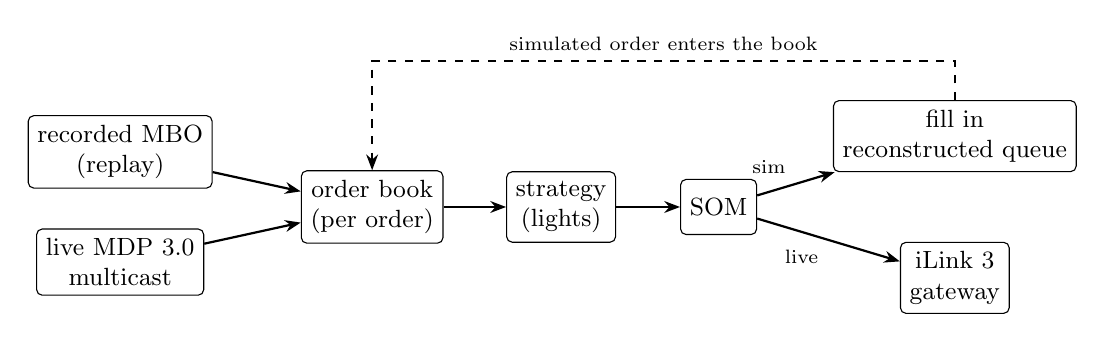
\begin{tikzpicture}[
  node distance=4mm and 6mm,
  box/.style={draw, rounded corners=2pt, minimum height=7mm, align=center, font=\small},
  arr/.style={-{Stealth[length=2mm]}, thick}]
\node[box] (md) at (0,0.7) {recorded MBO\\(replay)};
\node[box] (live) at (0,-0.7) {live MDP 3.0\\multicast};
\node[box] (ob) at (3.2,0) {order book\\(per order)};
\node[box] (strat) at (5.6,0) {strategy\\(lights)};
\node[box] (som) at (7.6,0) {SOM};
\node[box] (sim) at (10.6,0.9) {fill in\\reconstructed queue};
\node[box] (ilink) at (10.6,-0.9) {iLink 3\\gateway};
\draw[arr] (md) -- (ob);
\draw[arr] (live) -- (ob);
\draw[arr] (ob) -- (strat);
\draw[arr] (strat) -- (som);
\draw[arr] (som) -- node[above left, font=\scriptsize]{sim} (sim);
\draw[arr] (som) -- node[below left, font=\scriptsize]{live} (ilink);
\draw[arr, dashed] (sim.north) |- ++(0,5mm) -| node[pos=0.25, above, font=\scriptsize]{simulated order enters the book} (ob.north);
\end{tikzpicture}
\caption{Kaspar data and order paths. Everything downstream of the market-data source is the same
code in replay and live operation; the branch between simulated and live execution is a single
decision in the simulated order manager.}
\label{fig:kaspar}
\end{figure}

% ================================================================
\section{Queue-exact simulated fills}
\label{sec:kaspar-fills}
% ================================================================

The central requirement of Section~\ref{sec:replay} is that a simulated order should be filled only if
a real order in its place would have been. This section explains how Kaspar meets it: simulated
orders sit in the same per-order queue as real ones, reach the book after a modelled delay, and are
filled only by real executions that reach them. Here and throughout, \emph{queue-exact} means exact
with respect to the displayed order sequence carried by the input MBO feed and the documented matching
rules; it does not imply knowledge of hidden liquidity or unobserved participants, and it does not model
the market impact of the simulated orders.

\subsection{The book holds every order}

The simulator reconstructs a full market-by-order book from recorded exchange data. Each price
level is a queue that holds every resting order individually, in arrival order, and simulated
orders are held in the same queue alongside real ones. There is no estimated ``volume ahead''
variable: a simulated order's queue position is its position in the list. This is the property
that makes a fill inference definable at all~\citep{maciejewski_shadow}.

\subsection{Placement and latency}

In simulation mode the SOM turns a new order into a book \emph{add} message tagged with a
simulated venue identifier and sends it to the order-book actor. The book does not insert it
immediately. It holds the order on a delay queue until its modelled arrival time at the matching
engine:
\begin{lstlisting}[language=C++]
auto order_engine_arrive_time =
    order_leave_time
      + uint64_t(feed_delay) * 1000
      + uint64_t(std::max(40, eff_delay)) * 1000; // 40 us floor
\end{lstlisting}
The outbound order delay, the outbound cancel delay and the inbound feed delay are independent
parameters. The feed delay is added because the strategy saw the market late by that amount, so a
round trip is feed plus order, not order alone. When the order arrives it is appended at the tail
of the queue at its price, behind all depth already resting there.

\subsection{The fill rule}

A recorded cancellation of a real order simply unlinks it, and every order behind it moves up. A
recorded execution triggers simulated fills only when the executing real order is the first real
order in the queue and a simulated order sits ahead of it:
\begin{lstlisting}[language=C++]
// fill sim orders only if the executing order is at the front
if (o == q->get_head_no_sim())
{
  fill_prev_sim_order();
  ...
}
\end{lstlisting}
Any remaining executed quantity is carried forward to earlier simulated orders. This is the
price--time-priority argument of Section~\ref{sec:replay} in code: an aggressor that reached a
real order which arrived after the simulated order must have passed through the simulated order.
Simulated orders are excluded from the best bid and offer that the strategy sees, so a strategy
cannot react to its own quote. Market impact is not modelled~\citep{maciejewski_shadow}.

\begin{example}[A fill, step by step]
\label{ex:trace}
Bid queue at 5000.00 over seven successive steps \#0--\#6, sizes in lots, real orders R1--R4 and
one simulated order S:
\begin{lstlisting}
#0  resting:            R1(10) R2(5) R3(20)
#1  S(3) arrives:       R1(10) R2(5) R3(20) S(3)      appended at tail
#2  R2 cancels:         R1(10) R3(20) S(3)            S moves up
#3  exec 10 vs R1:      R3(20) S(3)                   no sim order ahead of R1: no fill
#4  exec 20 vs R3:      S(3)                          S is behind R3: no fill
#5  R4(8) joins:        S(3) R4(8)
#6  exec 5 vs R4:       R4 is head real, S ahead  ->  S filled 3 @ 5000.00
\end{lstlisting}
At step \#6 the aggressor reached R4, which arrived after S, so it must have passed through S. A
``touch'' backtest would have filled S at step \#3, three recorded events earlier and before the
queue ahead of it was consumed.
\end{example}

\paragraph{Market impact: a limitation of replay, and a possible extension.} Because the recorded
market behaves exactly as it did, whatever the simulated orders do, replay answers ``would my order have
been filled against this market?'' but not ``how would the market have moved because of my order?''. A
simulated order never consumes liquidity that real traders would have reacted to. Market impact is
therefore outside what this architecture measures, and it is not implemented.

One way to add a reacting market, which we describe as possible future work rather than a feature, is a
second market-data source: a queue-reactive simulator (Section~\ref{sec:qr}) in place of the recorded feed.
The separation between the source of market data and the book, order manager and strategy actors means
the rest of the pipeline would not change. The generator produces queue counts rather than individual
orders, so its events would have to be turned into synthetic order-level messages---order identifiers and
first-in-first-out placement---for the existing book. The researcher's orders would then change queue
sizes, the simulator's rates would respond, and the price response to the strategy's own trading could be
measured.

What such an extension would estimate is limited, and should be stated with it.
\begin{itemize}[leftmargin=1.5em,itemsep=1pt]
\item It would capture \emph{mechanical} impact: queues consumed by the strategy's orders, refilling at
  state-dependent rates, and price moves when a queue empties. Neural extensions of the queue-reactive
  model reproduce the square-root law of impact on Bund futures~\citep{deepqr}, so this part can be
  realistic.
\item It would not capture \emph{informational} impact: other participants inferring that a large buyer is
  present and repricing. In the queue-reactive model this sits in the random resets of the book, which do
  not respond to the strategy, and for large orders it is a substantial part of real impact.
\item Its impact would be a property of the simulator, and would need checking against impact measured on
  real trading---post-fill mark-outs from paper or live fills, or published impact laws---before being
  relied on.
\end{itemize}
The resulting division of labour would be: queue-exact replay for fill realism on the real market, without
impact; a reactive simulator for mechanical impact and for comparing tactics in a market that responds;
and paper and live trading as the ground truth for both.

% ================================================================
\section{The replay pipeline}
\label{sec:kaspar-pipeline}
% ================================================================

A traditional backtester reads bars or trades from a file and applies a fill rule to a strategy's
orders. A queue-exact replay must instead reproduce the market data exactly as the trading system
would have received it, so that the same code path builds the same book. Kaspar supports three market-data
sources, each feeding the same downstream code:

\begin{center}\footnotesize
\begin{tabularx}{\linewidth}{>{\raggedright\arraybackslash}X>{\raggedright\arraybackslash}X>{\raggedright\arraybackslash}p{0.2\linewidth}}
\toprule
Source & Reader & Clock \\
\midrule
Live CME MDP~3.0 multicast & socket reader & real time \\
Packet capture (\texttt{.pcap}) of the same multicast groups & PCAP reader & capture timestamps \\
Decoded order-by-order record file & binary file reader, directly into the books & file timestamps \\
\bottomrule
\end{tabularx}
\end{center}

\begin{figure}[ht]
\centering
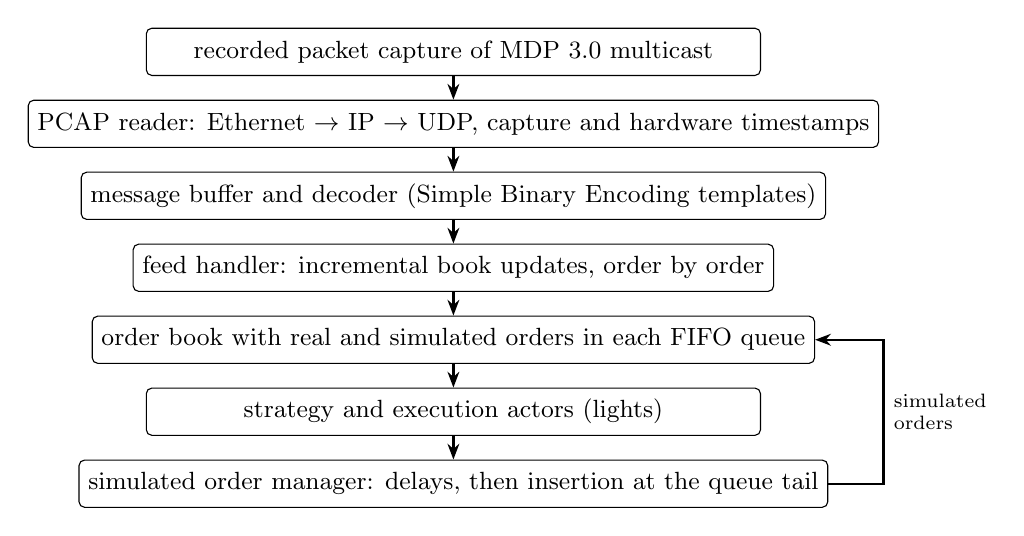
\begin{tikzpicture}[
  node distance=3mm,
  box/.style={draw, rounded corners=2pt, minimum width=78mm, minimum height=6mm, align=center, font=\small},
  arr/.style={-{Stealth[length=2mm]}, thick}]
\node[box] (a) {recorded packet capture of MDP~3.0 multicast};
\node[box, below=of a] (b) {PCAP reader: Ethernet $\to$ IP $\to$ UDP, capture and hardware timestamps};
\node[box, below=of b] (c) {message buffer and decoder (Simple Binary Encoding templates)};
\node[box, below=of c] (d) {feed handler: incremental book updates, order by order};
\node[box, below=of d] (e) {order book with real and simulated orders in each FIFO queue};
\node[box, below=of e] (f) {strategy and execution actors (lights)};
\node[box, below=of f] (g) {simulated order manager: delays, then insertion at the queue tail};
\foreach \x/\y in {a/b,b/c,c/d,d/e,e/f,f/g} \draw[arr] (\x) -- (\y);
\draw[arr] (g.east) -- ++(7mm,0) |- node[pos=0.25, right, font=\scriptsize, align=left]{simulated\\orders} (e.east);
\end{tikzpicture}
\caption{The packet-level replay path. Every stage below the reader is the same code that runs on
live data; only the reader and the final branch of the order manager differ.}
\label{fig:pcap}
\end{figure}

The capture reader parses each packet down to the exchange payload, optionally strips a
hardware-timestamp trailer added by capture equipment, and hands the payload to the same message
buffer the live socket reader uses, with both the software and hardware timestamps. It reads one
packet per message to itself, so replay is an ordinary actor loop rather than a blocking file read.
Two limits are stated in the project documentation: capture replay performs no packet recovery or
A/B feed arbitration, so a gap in the capture propagates to the book; and the decoded-record path
bypasses decoding entirely and is the fast option for repeated backtests. In the distributed
version, the capture and record readers are complete as libraries but not yet selectable from the
trading binary's command line; the separate simulator program drives replay from decoded record
files.

The order book then holds every order individually (Section~\ref{sec:kaspar-fills}), so a simulated
order's queue position is exact, and fills are decided by the recorded executions that follow.

% ================================================================
\section{Determinism}
\label{sec:kaspar-determinism}
% ================================================================

In the replay configuration the file reader, the order book, the timer, the SOM, the strategy
actors and the position manager all run in one actor group on one thread. The reader is added to
the group last, so all consumers exist before the first market-data message is delivered. Three
design choices then make a replay repeatable:
\begin{enumerate}[leftmargin=1.5em]
\item \textbf{One message sequence.} A single thread processes every message---market data, orders,
  acknowledgements, fills, timer events---in one total order.
\item \textbf{Market time.} The timer actor is driven by market-data timestamps, not the wall
  clock, so timeouts fire at the same point in the data on every run.
\item \textbf{Seeded randomness.} Any randomised strategy decision uses a per-actor seeded
  generator set in configuration.
\end{enumerate}
The property this implies, and the test that would check it, is that replaying the same recorded
file twice with the same configuration yields byte-identical fill records. We argue the property
from the design; we do not report the test here.

Determinism addresses a common weakness of trading research: the research implementation and the
production implementation are often different programs, and differences between them are
discovered in production.

% ================================================================
\section{Replay, paper and live equivalence}
\label{sec:kaspar-equivalence}
% ================================================================

Two choices are independent: where market data come from (recorded file or live multicast), and
where orders go (reconstructed book or exchange). Everything downstream of the message buffer---the
decoder, feed handler, order book, strategy and SOM---is the same code whichever source feeds it.
The branch between simulated and live execution is a single condition in the SOM's new-order
handler; both paths apply the same pre-trade reject checks, with one additional rule in live mode
for cancels of orders not yet acknowledged by the exchange. The combination ``live data, simulated
execution'' is paper trading: orders enter the live reconstructed book and are filled by the live
order flow under the same rule as in replay.

The live order-entry path implements CME's iLink~3 protocol: binary message encoding, HMAC request
signing, sequence management, and failover between primary and secondary gateways. The project
documentation states that both the market-data handler and the order-entry session have passed CME's
automated certification. Strategies can be written as in-process actors in C++ or, through an
in-process foreign-function interface, in Rust.

Two qualifications keep the claim precise. Switching between simulated and live execution is a single
flag in the SOM, but in the distributed build that flag is set in the program source rather than in a
configuration file, and the distributed configuration runs in simulation mode; the equivalence
demonstrated day to day is therefore between replay and paper trading, with the live path sharing all
code up to the SOM branch. And equivalence of code is not equivalence of outcomes: replay assumes no
market impact (Section~\ref{sec:kaspar-fills}) and models latency with configured delays, so a strategy
that is profitable in replay can still behave differently live.

% ================================================================
\section{A model-free execution benchmark}
\label{sec:shadow}
% ================================================================

\pov{} is the passive execution algorithm used in the case study~\citep{maciejewski_shadow}. It
makes no prediction about book evolution. When a third-party limit order is added within a
configured distance of the touch, the algorithm may place its own order at the same price, records
that participant's exchange order identifier, and cancels when that order leaves the book. The
placement decision is randomised at a configured rate; cancellation can be delayed by a grace
period measured in events or time. The design comment for the grace period states the trade-off
of Section~\ref{sec:adverse} directly: cancel too quickly and fills are given up; cancel too
slowly and the order bears the adverse selection.

\begin{table}[!htbp]
\centering\small
\caption{Representative \pov{} parameters (one of the configurations in the code repository).}
\label{tab:shadow-params}
\begin{tabular}{lll}
\toprule
Parameter & Value & Meaning \\
\midrule
\texttt{place\_rate\_bp} & 300 & place on 3\% of qualifying third-party adds \\
\texttt{max\_dist} / \texttt{max\_dist\_cancel} & 10 / 12 & ticks from touch to place / to force cancel \\
\texttt{delayed\_cancel\_events} & 5 & grace period after the shadowed order leaves \\
\texttt{nlights\_per\_side} & 10 & number of lights per side; each holds one order at one price \\
\texttt{rng\_seed} & 1 & seed for the placement decision \\
\bottomrule
\end{tabular}
\end{table}

Its role in this survey is as a null model for passive placement. It defines the bottom rung of a
hierarchy:
\begin{center}
model-free placement $\;\to\;$ predictive placement $\;\to\;$ full predictive execution policy.
\end{center}
A predictive model that claims value for passive execution should beat the model-free benchmark
\emph{in the same replay, under the same fill rule}, on slippage and on post-fill mark-outs. Any
improvement measured against a naive backtest instead is confounded by the fill-inference bias
of Section~\ref{sec:replay}.

% ================================================================
\section{Measurement}
\label{sec:kaspar-measurement}
% ================================================================

Latency claims need their endpoints. In the published measurement of Kaspar's market-data
handler, the start point is a software timestamp at the socket read and the end point is the order
book being published; time spent in the network card and kernel before the read is outside the
measurement, which is therefore socket-to-book, not wire-to-book. Measured on live CME multicast,
the median is 8.0\,$\mu$s, with book-message medians of 7.1, 7.3 and 7.1\,$\mu$s for ES, NQ and ZN
and 99th percentiles of 18.5, 13.6 and 57.0\,$\mu$s~\citep{maciejewski_mdlatency}. These numbers are
quoted as an example of stating endpoints, not as a result of this paper.

The simulator's slippage instrumentation measures execution cost for each fill against four
references: the mid at decision time, the interval volume-weighted average price, same-side
passive fills by other participants, and the touch. Comparing against the interval VWAP separates
market drift from adverse selection. Post-fill mark-outs at fixed times and after a fixed number
of book events provide the mark-out $R^{\text{fill}}_{h}$ of~\eqref{eq:markout} (the event-count version is
its analogue on an event clock) and the adverse-selection quantity of Section~\ref{sec:adverse}.

The order-flow signals of Part~II---OFI, queue imbalance, micro-price, fill-probability
models---are not part of the system described here. They are the candidate inputs that
Part~V proposes to search over, using this replay as the evaluator.


\part{LLM-Assisted Model Discovery}
\paragraph{About this part.} Language models can now write code, propose features and suggest model
structures. Part~V asks how that ability fits into the research process of the previous parts without
corrupting it. It first separates three different uses of generative models in LOB research
(Section~\ref{sec:three-uses}); then describes \lamd{}, a loop in which a language model proposes
candidate models and a deterministic replay judges them (Section~\ref{sec:lamd}); explains why a
proposal from a language model is not evidence (Section~\ref{sec:not-validation}); distinguishes
searching a fixed space from inventing explanations (Section~\ref{sec:abduction}); and shows how the
number of candidates tried raises the bar any winner must clear (Section~\ref{sec:search}).

% ================================================================
\section{Three uses of generative models, kept apart}
\label{sec:three-uses}
% ================================================================

Generative and language-model technology now enters LOB research in at least three distinct ways,
and they should not be confused.

\begin{table}[!htbp]
\centering\small
\caption{Three uses of generative models in LOB research.}
\label{tab:three-uses}
\begin{tabularx}{\linewidth}{lXXl}
\toprule
Use & What is generated & Examples & In this paper \\
\midrule
LOB generation & synthetic order and message streams & autoregressive message
  models~\citep{nagy2023} and their evaluation benchmarks~\citep{lobbench2025} & adjacent work \\
LOB modelling & predictions and representations of market state & Transformers, state-space models,
  pretrained encoders~\citep{linna2025lobert} & Part~II \\
Model generation & candidate models, signals and hypotheses & \lamd{} & this part \\
\bottomrule
\end{tabularx}
\end{table}

LOB generation produces market trajectories; the generated messages can be processed by a book
simulator to produce synthetic books. Its value lies in simulation, stress testing and data
augmentation, and its difficulty lies in preserving the joint structure of orders, queues,
executions and prices rather than only their marginal statistics. It is a legitimate research area
but not part of the methodology proposed here: consistent with the first principle of
Section~\ref{sec:intro}, candidate models are evaluated only on observed market data.

A fourth use is now large enough to have its own surveys: the language model as a \emph{trading agent}.
\citet{ding2024llmtrading} review LLM agents for financial trading---their architectures, data inputs,
backtest performance and open challenges---and \citet{dong2025llmfinance} survey LLM agents across five
financial domains (data analysis, investment research, trading, investment management and risk
management), cataloguing over 30 financial benchmarks and 20 representative models and the obstacles to
deployment. \citet{hua2026agentic} review \emph{agentic} quantitative trading across five stages---factor
mining, signal discovery, portfolio construction, order execution and risk management---and find that
current systems concentrate on signal discovery, that integration with execution and risk control is
still uncommon, and that strong model or forecasting capability ``does not reliably translate into
trading performance under live market conditions''. That literature asks how a language model can act
in markets. This part asks a narrower
question: how a language model can take part in quantitative hypothesis generation without becoming
either the source of the market data or the source of the evidence that validates a hypothesis.

LOB modelling is the subject of Part~II. A pretrained encoder that can also predict the next
message, such as LOBERT, is used there as a model of the market, not as a source of data.

Model generation is different in kind. The language model does not produce market data or market
forecasts. It produces \emph{hypotheses about how to trade}, which are then evaluated against the
recorded market.

% ================================================================
\section{The \lamd{} loop}
\label{sec:lamd}
% ================================================================

LLM-Assisted Model Discovery (\lamd)\footnote{An earlier description of the same loop used the
name LLM-Assisted Trading Strategy Search (LATSS)~\citep{mayeski_latss}.} is a research loop in which a language model proposes
candidate models and every other step is external to it and reproducible: given the same data,
configuration and random seeds, it gives the same result. It belongs to a broader
family of methods in which a language model is paired with an automated evaluator to search a
space of programs~\citep{romera2024}. The closest published application in finance is
\citet{kou2025strategy}, in which prompted language models generate executable alpha-factor
candidates, agents filter them by market state and predictive quality, and the surviving factors are
combined with dynamically optimised weights; the authors report a 53.17\% cumulative return on the SSE~50
from January 2023 to January 2024, ahead of their benchmarks. The difference from
\lamd{} lies less in the generation step than in what surrounds it: \lamd{} makes the number of
candidates tried part of the evidence (Section~\ref{sec:search}) and, as proposed here for order-book
strategies, evaluates each candidate's execution in queue-exact replay on recorded order-level data; the
existing implementation~\citep{mayeski_latss} works on daily data. The components are:

\begin{enumerate}[leftmargin=1.5em]
\item \textbf{Vocabulary.} A human-specified set of primitives the proposals may use: OFI at several
  windows, queue imbalance, trade flow, Hawkes intensities, returns and volatility, queue position,
  regime indicators, cross-asset inputs, and execution actions (place, keep, cancel, cross).
\item \textbf{Proposal.} The language model proposes or mutates a candidate: a feature combination,
  a transformation, a decision rule or a model structure, expressed in the vocabulary.
\item \textbf{Compilation.} A deterministic compiler turns the proposal into an executable model
  with explicit free parameters. Proposals that do not compile are rejected without evaluation.
\item \textbf{Fitting.} Parameters are fitted on a training window only.
\item \textbf{Replay.} The fitted model drives an execution policy in a queue-exact replay of
  recorded data (Part~IV), against the model-free benchmark of Section~\ref{sec:shadow}.
\item \textbf{Validation.} Walk-forward out-of-sample evaluation with purging and embargo
  (Section~\ref{sec:validation}).
\item \textbf{Certification.} The out-of-sample result is compared against a null that accounts for
  every candidate evaluated so far (Section~\ref{sec:search}).
\item \textbf{Archive.} Every candidate---prompt, compiled model, fit, split, result---is recorded,
  whether it passed or failed, and the archive seeds the next round of proposals. The running count
  of candidates evaluated is $N_{\text{trials}}$.
\end{enumerate}

\begin{figure}[ht]
\centering
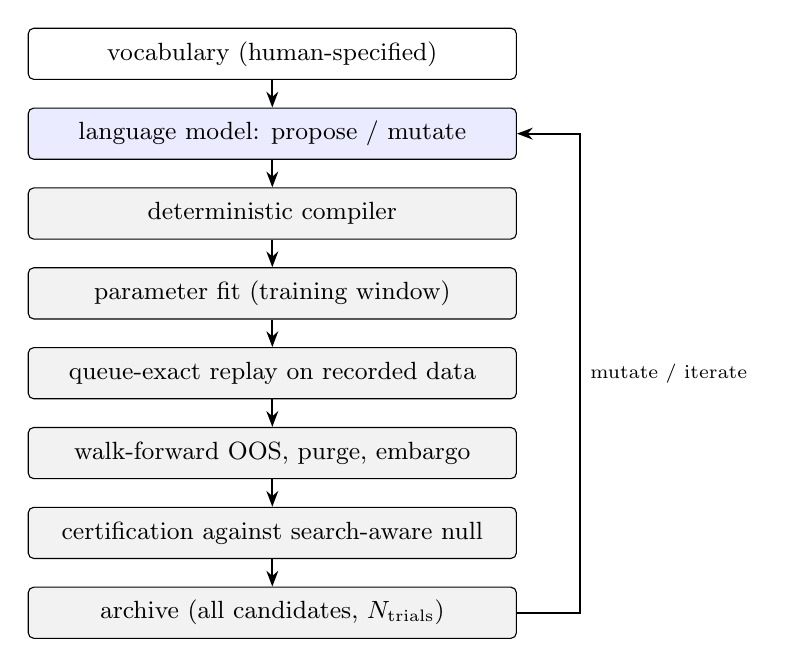
\begin{tikzpicture}[
  node distance=3.5mm,
  box/.style={draw, rounded corners=2pt, minimum width=62mm, minimum height=6.5mm, align=center, font=\small},
  llm/.style={box, fill=blue!8},
  det/.style={box, fill=gray!10},
  arr/.style={-{Stealth[length=2mm]}, thick}]
\node[box] (v) {vocabulary (human-specified)};
\node[llm, below=of v] (p) {language model: propose / mutate};
\node[det, below=of p] (c) {deterministic compiler};
\node[det, below=of c] (f) {parameter fit (training window)};
\node[det, below=of f] (r) {queue-exact replay on recorded data};
\node[det, below=of r] (o) {walk-forward OOS, purge, embargo};
\node[det, below=of o] (s) {certification against search-aware null};
\node[det, below=of s] (a) {archive (all candidates, $N_{\text{trials}}$)};
\foreach \x/\y in {v/p,p/c,c/f,f/r,r/o,o/s,s/a} \draw[arr] (\x) -- (\y);
\draw[arr] (a.east) -- ++(8mm,0) |- node[pos=0.25, right, font=\scriptsize]{mutate / iterate} (p.east);
\end{tikzpicture}
\caption{The \lamd{} loop. Only the shaded blue step involves the language model; every step that
touches data or produces evidence is a fixed, reproducible procedure.}
\label{fig:lamd}
\end{figure}

\begin{example}[One hypothetical iteration, three candidates]
In the table, $\OFI^{(5)}_t$ is $\OFI^{(w)}_t$ with $w = 5$ s; $\lambda_{\text{sell}}(t)$ is the
component $\lambda_i(t)$ of a fitted Hawkes model for which $i$ is the sell-market-order type, and
$\bar\lambda_{\text{sell}}$ the corresponding component of $\bar\lambda$; $\xi$ and $c$ are
thresholds fitted on the training window.
\begin{center}\small
\begin{tabularx}{\linewidth}{lXlll}
\toprule
id & proposal (paraphrased) & compiled form & OOS net, ticks/fill & $N_{\text{trials}}$ \\
\midrule
c1 & keep a passive bid only while short-horizon OFI agrees & cancel if $\OFI^{(5)}_t < \xi$ & $+0.04$ & 1 \\
c2 & interact OFI with queue imbalance & logit on $\OFI^{(5)}_t \times \QI_t$ & $+0.01$ & 2 \\
c3 & cancel faster when sell-order intensity spikes & cancel if $\lambda_{\text{sell}}(t) > c\,\bar\lambda_{\text{sell}}$ & $-0.02$ & 3 \\
\bottomrule
\end{tabularx}
\end{center}
Each result is measured relative to the model-free benchmark in the same replay. Candidate c1 is
not ``discovered'' when it tops this table; it is discovered only if it clears a null adjusted to
the total number of candidates the loop has evaluated, which after a few days of automated search
may be in the tens of thousands.
\end{example}

\subsection{A worked implementation}

The loop has been implemented for daily-frequency strategies in the LATSS system described
in~\citet{mayeski_latss}, and the details show which choices matter.
\begin{itemize}[leftmargin=1.5em,itemsep=1pt]
\item \textbf{The language model writes structure, never sees prices.} It composes transformations from
  a fixed set of fifteen tools (moving averages, rate of change, z-scores, realised volatility,
  breakouts, percentile ranks, crossovers and similar). Prices reach the code only when the engine
  runs it. Everything the system can discover is some arrangement of those tools.
\item \textbf{The model declares parameters; an optimiser sets them.} Every window and threshold is a
  declared ``knob'' with a range; differential evolution chooses its value on training data.
\item \textbf{Validation is fold-based.} Data are split by quarter; candidates are fitted on some
  quarters and scored on the held-out rest, and the median is kept. The author notes two weaknesses:
  long look-back windows leak a little information across fold boundaries, and random quarters
  resample a single regime, which missed a later regime change.
\item \textbf{The skill bar is empirical.} Each candidate's positions are circularly shifted in time,
  which keeps their exposure and turnover but scrambles their timing; the best score achieved by
  these skill-free shifted versions is the bar a candidate must clear.
\end{itemize}
The author's own assessment is the right one for this survey: with a generic vocabulary the results
are generic, and the human decisions---what to look for, which tools to supply, how hard to test, what
to trust---remain the binding constraints. For LOB models the vocabulary would be the primitives of
Part~II, and the evaluator the queue-exact replay of Part~IV.

% ================================================================
\section{Hypothesis generation is not validation}
\label{sec:not-validation}
% ================================================================

A candidate proposed by a language model has no stronger evidentiary status than one proposed by a
person. Its plausibility, its fluency, and the quality of the explanation that accompanies it are
not evidence that it captures market structure. The scientific content of \lamd{} is in the
deterministic steps around the proposal, not in the proposal.

The same caution applies to language models used directly on market data.
\citet{llmlob2026} train a language model on synthetic LOB event sequences and find that it
generates valid sequences almost perfectly, yet its implicit world model fails to learn the state
of the book, which leads to biased estimates and spurious predictability when it is used to
forecast events. Syntactic validity is not evidence of a learned mechanism, and the same holds for
plausible-looking trading rules. Only external evaluation on held-out observed data can establish that a
candidate works.

% ================================================================
\section{Search versus abduction}
\label{sec:abduction}
% ================================================================

A distinction from the philosophy of science clarifies what such a system can and cannot do.
\emph{Search} explores a given space of hypotheses: ``here is a space of possible solutions; try
things''. \emph{Abduction} creates a hypothesis that was not in the space: ``something about reality
does not make sense; what new concept would make sense of it?''~\citep{mayeski2026abduction}. Language
models are effective at search and recombination: program-search systems built on them have found new
mathematical constructions~\citep{romera2024}, and \lamd{} finds new arrangements of supplied tools.
\citet{zahavy2026} argues that current language models handle induction and, increasingly,
deduction, but lack a mechanism for the abductive step from experience to new principles.

For order-book research the implication is concrete. A \lamd{}-style system can search exhaustively
over combinations of known primitives---OFI at several windows, queue imbalance, Hawkes intensities,
queue position, state modulators, targets and horizons---far faster than a person. A system restricted
to such a vocabulary cannot discover a primitive outside it: a new state variable, an unrecognised
interaction between hidden and visible liquidity, or a new relation between depletion and adverse
selection. A less constrained system could, in principle, search over representations as well as over
combinations of supplied primitives; whether current language models can do so reliably is an empirical
question. Whether that limitation is permanent is an open question; that it holds for present systems
is the working assumption of this survey~\citep{mayeski2026agent}. Automated search is an amplifier of
human-specified structure, and its outputs must pass the same certification as any human proposal.

% ================================================================
\section{Search complexity and multiple testing}
\label{sec:search}
% ================================================================

The more candidates a search evaluates, the larger the best in-sample result it will find by
chance. For $N_{\text{trials}}$ independent candidates with no skill, the expected maximum of
their standardised Sharpe-ratio estimates grows roughly like $\sqrt{2 \ln N_{\text{trials}}}$. (The Sharpe ratio is
average return divided by the standard deviation of return---profit per unit of risk.) In words:
toss a thousand fair coins a hundred times each, and the luckiest coin will look like a skilled
one; the more coins, the luckier the best one looks, though the growth is slow. The deflated Sharpe
ratio~\citep{bailey2014} makes the correction precise and accounts for non-normal returns
(Section~\ref{sec:generalisation}). Related tools include the reality check for data
snooping~\citep{white2000}, the probability of backtest overfitting~\citep{bailey2014pbo}, and
raised significance thresholds for factor discovery~\citep{harvey2016}.

\begin{example}[The same Sharpe, different evidence]
Take the standard error of an annualised Sharpe estimate as approximately $1/\sqrt{T_{\text{yr}}}$ for $T_{\text{yr}}$
years of data, so the null maximum is about $\sqrt{2\ln N_{\text{trials}}}/\sqrt{T_{\text{yr}}}$:
\begin{center}\small
\begin{tabular}{rcc}
\toprule
$N_{\text{trials}}$ & null maximum, 1 year & null maximum, 4 years \\
\midrule
1 & 0 & 0 \\
100 & $\approx 3.0$ & $\approx 1.5$ \\
50\,000 & $\approx 4.65$ & $\approx 2.3$ \\
\bottomrule
\end{tabular}
\end{center}
A Sharpe ratio of 2 from a single pre-specified test on four years is evidence. The same Sharpe
ratio as the best of 50\,000 automatically generated variants on four years is below what noise
alone is expected to produce.
\end{example}

Automated proposal therefore changes the evaluation problem from ``performance and model
complexity'' to
\begin{equation}
  \boxed{\ \text{performance} \;+\; \text{model complexity} \;+\; \text{search complexity}\ }
\end{equation}
\inwords{to judge a discovered model you need three things, not one: how well it did, how
complicated it is, and how many other candidates were tried before it was found.}
The archive's trial count is as much a part of the result as the out-of-sample Sharpe ratio.
Faster replay makes this worse, not better: an order-of-magnitude increase in simulation speed is an
order-of-magnitude increase in the number of hypotheses that can be tested, and the skill threshold
must rise with it.

The central research question for automated model discovery is thus not whether an AI system can
generate a profitable-looking model, but whether an automated search can discover economically
significant structure while controlling the false-discovery rate that the search itself induces.


\part{Evaluation}
\paragraph{About this part.} Every earlier part ends with the same question: \emph{is the model any
good?} Part~VI answers it. Evaluation in this field fails in predictable ways---a metric that rewards
the wrong thing, a test set that leaks information from the training set, or a winner chosen from
thousands of tries that only looks good by chance---and each section addresses one of them. In order:
\begin{itemize}[leftmargin=1.5em,itemsep=1pt]
\item which \emph{statistical} scores measure forecast quality honestly, and why accuracy and F1 are
  not enough (Section~\ref{sec:stat-metrics});
\item how to measure \emph{economic} value---profit after costs, fills and adverse selection---which is
  what a forecast is ultimately for (Section~\ref{sec:econ-metrics});
\item how to split time-ordered data so that the test really is unseen (Section~\ref{sec:validation});
\item why more complex models need more evidence, and how to correct for having tried many models
  (Section~\ref{sec:generalisation});
\item how to choose between models of different complexity, which turns Occam's razor (Principle~3)
  into a procedure (Section~\ref{sec:parsimony});
\item and what a benchmark result must report for others to compare and reproduce it
  (Section~\ref{sec:benchmark}).
\end{itemize}
The thread through all six is the distinction of Part~I: a forecast is judged first as a forecast, then
as a trading input, and the second judgement is the one that matters.

% ================================================================
\section{Statistical metrics}
\label{sec:stat-metrics}
% ================================================================

The right statistical metric depends on the target (Table~\ref{tab:metrics}). These metrics
measure predictive quality; none of them, by itself, measures trading value.

\begin{table}[!htbp]
\centering\small
\caption{Statistical metrics by prediction target.}
\label{tab:metrics}
\begin{tabularx}{\linewidth}{lX}
\toprule
Target & Metrics \\
\midrule
Direction & log loss, Brier score~\citep{brier1950}, AUC~\citep{fawcett2006}, balanced accuracy, calibration error~\citep{guo2017} \\
Direction with confidence & risk--coverage curves; F1 by confidence tier; interval coverage against
  nominal (e.g.\ the 68\% coverage reported by~\citet{manoharan2026uqlob}) \\
Return & MSE, MAE, CRPS~\citep{gneiting2007} \\
Event time or fill & right-censored log-likelihood~\citep{arroyo2024}; calibration by queue-position bucket; concordance with caution \\
Intensity & point-process log-likelihood; time-rescaling residual tests \\
\bottomrule
\end{tabularx}
\end{table}

\paragraph{Proper scoring rules.} A scoring rule is \emph{proper} if a forecaster minimises the expected
score by reporting their true beliefs~\citep{gneiting2007}. Log loss, the Brier score and the CRPS are
proper; accuracy and F1 are not, because they reward only the side of a threshold a forecast falls on.
For any model whose output will be used as a probability---for sizing, for the confidence gating of
Section~\ref{sec:tradeability}, or for the fill-probability term of execution value---a proper score
should be the primary statistical metric, and calibration should be checked directly (events forecast
at 70\% should happen about 70\% of the time). For fill-time models, censoring by cancellations makes
some familiar survival metrics improper; the right-censored log-likelihood is the safe
choice~\citep{arroyo2024}.

% ================================================================
\section{Economic metrics}
\label{sec:econ-metrics}
% ================================================================

Economic evaluation starts from the aggressive and passive returns of Section~\ref{sec:passive} and
the decomposition 
\[
  \E[\Pi^{\text{pass}}] = \P(\Fill)\,\E[\Pi^{\text{pass}} \mid \Fill],
\]
which separates execution probability
from conditional execution quality. For passive strategies both factors should be reported, broken
down by queue position where the data allow.

Table~\ref{tab:metric-levels} orders evaluation metrics by how close they come to trading value. A
study should say which levels it reaches; most LOB papers stop at the first or second.

\begin{table}[!htbp]
\centering\footnotesize
\caption{Levels of evaluation, from statistical to economic.}
\label{tab:metric-levels}
\begin{tabularx}{\linewidth}{l>{\raggedright\arraybackslash}X>{\raggedright\arraybackslash}X}
\toprule
Level & Question & Typical metrics \\
\midrule
Prediction & Is the direction or value right? & accuracy, F1, AUC, MSE \\
Probabilistic prediction & Are the stated probabilities right? & log loss, Brier, CRPS, calibration \\
Execution & Will the order trade? & fill probability, fill-time likelihood \\
Conditional execution & How good is the trade when it happens? & mark-outs, adverse selection by queue position \\
Trading & Does it make money after costs? & net P\&L, Sharpe ratio, transaction-level overlap $\mathrm{TO}$~\citep{briola2024} \\
Capacity & How much can be traded before impact erases it? & turnover, impact-adjusted P\&L \\
Robustness & Does it survive new periods, assets and regimes? & out-of-sample by regime and asset \\
Statistical validity & Could the result be luck given the search? & deflated Sharpe ratio, null maximum, backtest-overfitting probability \\
\bottomrule
\end{tabularx}
\end{table}

Cost-aware directional metrics, which ask whether a predicted trade would have produced a favourable
executable outcome rather than whether the mid moved in the predicted direction, are an improvement
over raw accuracy. They are not a complete economic metric: they omit market impact, capacity,
inventory, repeated trading, the distribution of latency, and queue position in detail. In
Example~\ref{ex:as}, a metric that ignored $\P(\Fill)$ would misjudge the two positions. Such
metrics should be reported alongside realised trading metrics, not instead of them.

% ================================================================
\section{Temporal validation}
\label{sec:validation}
% ================================================================

Cross-validation with randomly assigned folds is inappropriate for most LOB problems because observations are
dependent in time. A chronological split preserves the direction of information flow, and
walk-forward evaluation repeats it. Where features and labels overlap in time, training samples
whose information overlaps the test period must be purged and an embargo imposed after each test
window~\citep{lopezdeprado2018}. The embargo should follow from the maximum look-back and the
forecast horizon, not be chosen arbitrarily.

\begin{example}[Sizing an embargo]
Features use a 60-second look-back and labels a 10-second horizon. The embargo at each
train/test boundary is at least 70 seconds. A walk-forward schedule might train on 20 sessions,
validate on 5 and test on 5, then roll forward by 5.
\end{example}

When several models are compared on the same data, a \emph{model confidence set}~\citep{hansen2011mcs}
identifies the subset that cannot be statistically distinguished from the best, at a stated
confidence level; it is the honest alternative to declaring the model with the highest score the
winner. Beyond a single test period, models should be stress-tested across volatility regimes, tick
and fee changes, and assets of different tick size, since predictability differs systematically
between large- and small-tick instruments~\citep{briola2024,gould2016qi}.

LOB research has large implicit search spaces: feature definitions, look-backs, horizons,
normalisations, thresholds, architectures, hyper-parameters, assets, sessions and execution
assumptions. When thousands of configurations are tried, the best one looks good by chance. Model
complexity and research-process complexity must be considered together
(Section~\ref{sec:search}).

% ================================================================
\section{Capacity, generalisation and multiple testing}
\label{sec:generalisation}
% ================================================================

A model that fits the training data well can still fail on new data, and the more flexible the
model, or the more models were tried, the more likely that is. This section gives the theory behind
that statement in three steps: why simpler model families generalise more reliably, how to correct a
performance measure for the number of models tried, and why simple models are also easier to test
honestly.

\subsection{Generalisation of simpler models}

Statistical learning theory makes the intuition behind Occam's razor precise. For a classifier $M$ chosen
from a family of models with \emph{VC dimension} $\mathrm{VC}$---roughly, the largest number of points
the family can label in every possible way---and trained on $N_s$ independent examples, with probability
at least $1-\varsigma$ the error rate on new data satisfies~\citep{vapnik1998}
\begin{equation}
  \text{err}(M) \le \widehat{\text{err}}_{N_s}(M) +
  \sqrt{\frac{\mathrm{VC}\,\big(\ln(2N_s/\mathrm{VC}) + 1\big) - \ln(\varsigma/4)}{N_s}} .
\end{equation}
\inwords{error on new data is at most the training error plus a penalty that grows with the
richness of the model family and shrinks with the amount of data. A richer family can fit more
patterns, including patterns that are only noise, and needs more data before its training error can be
trusted.} Rademacher complexity~\citep{bartlett2002}, which measures how well a model family can fit
random noise on the data actually observed, gives bounds of the same form that are never much worse than the VC bounds and can be tighter.

Two features of LOB data make the penalty bite. The signal is weak relative to the noise, so a family
that can fit noise will. And observations are strongly dependent in time, so the \emph{effective}
number of independent examples is far smaller than the number of events: a day of ES data has
millions of messages but far fewer independent price moves.

Two caveats keep the argument honest. Modern deep networks can fit even random labels perfectly and
still generalise on real labels~\citep{zhang2017rethinking}, and test error can fall again as capacity
grows past the point where the training data are fitted exactly (``double
descent'')~\citep{belkin2019}. Classical capacity bounds therefore do not decide by themselves whether
a deep model will generalise on LOB data. What decides it is out-of-sample evidence---which is why the
benchmark studies of Section~\ref{sec:benchmarks-dl} carry more weight than any bound.

\paragraph{Practical penalties.} Information criteria trade fit against parameter count explicitly:
the Akaike criterion adds twice the number of parameters to minus twice the log-likelihood~\citep{akaike1974},
and the Bayesian criterion adds the number of parameters times the logarithm of the sample
size~\citep{schwarz1978}, penalising complexity more heavily in large samples. The lasso adds a penalty
on the sum of absolute coefficients, which drives unhelpful coefficients exactly to zero and so selects
features automatically~\citep{tibshirani1996}. All three are applied to a single fit; none accounts for
the search that produced the model family in the first place, which is the subject of the next
subsection.

\subsection{Multiple testing and the deflated Sharpe ratio}

If $N_{\text{trials}}$ strategies with no skill are tested, and their estimated Sharpe ratios have
standard deviation $\sigma_{\text{SR}}$ across trials, the expected best estimate is
approximately~\citep{bailey2014}
\begin{equation}
  \E\big[\max \widehat{\text{SR}}\big] \approx \sigma_{\text{SR}}
  \left[(1-\gamma_E)\,\Phi^{-1}\!\left(1 - \frac{1}{N_{\text{trials}}}\right)
  + \gamma_E\, \Phi^{-1}\!\left(1 - \frac{1}{N_{\text{trials}}\, \mathrm{e}}\right)\right],
\end{equation}
where $\Phi^{-1}$ is the inverse of the standard normal distribution function, $\gamma_E \approx 0.5772$
is the Euler--Mascheroni constant and $\mathrm{e}$ is Euler's number.
\inwords{this is the Sharpe ratio that the luckiest of $N_{\text{trials}}$ worthless strategies is
expected to show. It grows with the number of trials, roughly like $\sqrt{2\ln N_{\text{trials}}}$; the
example of Section~\ref{sec:search} used that rough form.} Write this expected maximum as
$\text{SR}_0$. The \emph{deflated Sharpe ratio} is the probability that the selected strategy's true
Sharpe ratio exceeds $\text{SR}_0$, given its estimate $\widehat{\text{SR}}$ from $N_{\text{obs}}$
returns:
\begin{equation}
  \text{DSR} = \Phi\!\left(\frac{(\widehat{\text{SR}} - \text{SR}_0)\sqrt{N_{\text{obs}} - 1}}
  {\sqrt{1 - \widehat{\text{skew}}\;\widehat{\text{SR}} + \frac{\widehat{\text{kurt}} - 1}{4}\,\widehat{\text{SR}}^{\,2}}}\right),
\end{equation}
where $\widehat{\text{skew}}$ and $\widehat{\text{kurt}}$ are the sample skewness and (raw, not excess)
kurtosis of the returns and the Sharpe ratios are per period, not annualised.
\inwords{the numerator asks how far the observed Sharpe ratio is above what luck alone would produce
after this many trials; the denominator widens the uncertainty when returns are skewed or
fat-tailed. A DSR near 1 means the result is unlikely to be luck; near 0.5 or below, it is
indistinguishable from the best of a batch of noise.}

The same authors turn this into a budget. For a given length of history there is a maximum number of
configurations that can be tried before a strategy with no skill is expected to show an impressive
in-sample Sharpe ratio; with five years of data, ``no more than forty-five independent model
configurations should be tried'' if one wants to avoid an expected in-sample Sharpe ratio of 1 from a
strategy whose out-of-sample expectation is zero~\citep{bailey2014pseudo}. The probability of backtest
overfitting~\citep{bailey2014pbo}, White's reality check~\citep{white2000}, raised significance
thresholds~\citep{harvey2016} and false-discovery-rate control~\citep{benjamini1995} address the same
problem from different directions.

\subsection{Backtestability}

These tools favour simple models for a reason beyond generalisation: a simple model family is
\emph{backtestable}. When the family is small, the number of effective trials can be counted or
bounded, the null maximum can be computed, and the path from signal to decision can be audited. As the
family grows---deep networks with many hyper-parameters, richly parameterised point processes, or
automated search over model structures---the effective number of trials becomes hard to state, and with
it the bar a result must clear. Parsimony is therefore a property of the research process as well as of
the model.

% ================================================================
\section{Occam's razor as a model-selection principle}
\label{sec:parsimony}
% ================================================================

This section makes Principle~3 operational. We do not propose a single scalar penalty for
complexity. With $V(M)$ as in
Section~\ref{sec:notation}, let
\begin{equation}
  \mathcal{C}(M) = \left(\mathcal{C}_{\text{param}}(M),\, \mathcal{C}_{\text{lat}}(M),\,
  \mathcal{C}_{\text{fit}}(M),\, \mathcal{C}_{\text{mon}}(M),\, N_{\text{trials}}(M)\right)
\end{equation}
collect the dimensions of complexity: the number of fitted parameters, the inference latency, the
effort to fit and refit its parameters, the effort to monitor in production, and the number of
candidates $N_{\text{trials}}(M)$ searched to find the model (Section~\ref{sec:lamd}).
\inwords{complexity is a list of separate costs, not one number: how many knobs the model has, how
slow it is, how much work it is to tune and to watch, and how hard someone searched to find it.} A complex model
$M_1$ should be preferred to a baseline $M_0$ only if $\Delta V = V(M_1) - V(M_0)$ is statistically
credible and economically meaningful relative to 
\[
  \Delta\mathcal{C} = \mathcal{C}(M_1) - \mathcal{C}(M_0).
\]
Because the
components of $\mathcal{C}$ share no common unit, the framework asks for them to be reported separately
(Table~\ref{tab:parsimony}), so the reader can judge whether the added complexity is justified.

\begin{table}[!htbp]
\centering\small
\caption{Complexity dimensions of the model classes discussed in this survey, in orders of
magnitude. A comparison should add, for each row, the out-of-sample Sharpe ratio, the deflated
Sharpe ratio and the number of configurations tried, all under the same fill model.}
\label{tab:parsimony}
\begin{tabular}{llll}
\toprule
Model & Parameters & Typical inference latency & Fitting burden \\
\midrule
Model-free benchmark (\S\ref{sec:shadow}) & $\sim 10$ settings & $\mu$s & none \\
OFI baseline & $\sim 10$ & ns--$\mu$s & low \\
Shallow network & $10^3$--$10^4$ & $\mu$s & medium \\
Transformer & $\sim 10^6$ & ms & high \\
Hybrid & $\sim 10^6$ & ms & high \\
\bottomrule
\end{tabular}
\end{table}

\paragraph{An explicit exchange rate.} When a decision must be made, the separate dimensions can be
combined by stating, in advance, how much economic value each unit of added complexity must buy.
Writing $\Delta\mathcal{C}$ as a weighted sum of its components with weights chosen by the user, the
rule ``adopt $M_1$ only if $\Delta V > \chi\,\Delta\mathcal{C}$'' for a stated $\chi > 0$ makes
the trade-off explicit and auditable. The value of the rule lies in stating the weights before the
comparison, not in any particular choice of them.

\paragraph{Starting points ordered by complexity.} Table~\ref{tab:selection} orders candidate approaches by increasing
complexity, with the condition under which each is the natural starting point. It is a guide to where
the burden of proof lies, not a ranking of methods: a more complex row is justified when the simpler one
above it has been tried, on the same data and fill model, and found wanting.

\begin{table}[!htbp]
\centering\footnotesize
\caption{Starting points ordered by increasing complexity.}
\label{tab:selection}
\begin{tabularx}{\linewidth}{>{\raggedright\arraybackslash}p{0.24\linewidth}>{\raggedright\arraybackslash}X>{\raggedright\arraybackslash}X}
\toprule
Situation & Start with & Why \\
\midrule
Decision needed within microseconds; large-tick instrument & linear OFI or queue imbalance; queue-race probability (Section~\ref{sec:cdl}) & few operations, deterministic latency, strongest evidence in large-tick names~\citep{gould2016qi,briola2024} \\
Passive execution; fill probability matters & residual-volume and OFI baseline; then a survival model with queue position as an input~\citep{kanformer} & prices fill probability and adverse selection directly \\
Decision within milliseconds; liquid instrument & neural network on order-flow inputs~\citep{kolm2023,lucchese2024} & order-flow inputs carry most of the gain; in re-tests the simple MLP degraded least~\citep{prata2024} \\
Several horizons at once & sequence model only if baselines fail deflated and purged tests & complexity must clear the multiple-testing bar \\
Unusual volatility or liquidity & volatility gating of a simpler model & simple and robust when learned relations break \\
Several related instruments & lagged cross-asset OFI~\citep{contcucuringu2023} & modest complexity; evidence of forecasting value \\
\bottomrule
\end{tabularx}
\end{table}

\paragraph{A parsimony checklist.} The contrast between an over-engineered and a parsimonious approach
can be stated dimension by dimension (Table~\ref{tab:checklist}). The right-hand column is a default,
to be departed from with evidence.

\begin{table}[!htbp]
\centering\footnotesize
\caption{Over-engineered versus parsimonious defaults.}
\label{tab:checklist}
\begin{tabularx}{\linewidth}{l>{\raggedright\arraybackslash}X>{\raggedright\arraybackslash}X}
\toprule
Dimension & Over-engineered & Parsimonious default \\
\midrule
Features & many correlated indicators & a few interpretable drivers (OFI, imbalance, queue position) \\
Model & deep network chosen first & linear or logistic model first, then a shallow network \\
Fitting criterion & in-sample fit & out-of-sample economic value, with information criteria or shrinkage \\
Search & unrecorded trials & counted trials and a deflated result \\
Regime behaviour & fragile under shocks & degrades gracefully; gated by volatility \\
Diagnosis & opaque when it fails & failures traceable to an identifiable input \\
\bottomrule
\end{tabularx}
\end{table}

% ================================================================
\section{Benchmarking standard and datasets}
\label{sec:benchmark}
% ================================================================

A scientifically useful LOB benchmark should report at least the following.
\begin{description}[leftmargin=1.5em,style=nextline]
\item[Data] exchange; instrument; date range; number of sessions; L1, L2 or L3; event count; tick
  size; spread; depth.
\item[Prediction] target; horizon; sampling clock; feature look-back; normalisation.
\item[Model] architecture; parameter count; training procedure; hyper-parameter search;
  computational budget.
\item[Validation] chronological split; walk-forward procedure; purging; embargo; number of trials.
\item[Execution] latency; fees; spread; queue position; fill model; market-impact assumption.
\item[Results] statistical metric; economic metric; confidence interval; null benchmark;
  robustness across regimes.
\end{description}

Public datasets and frameworks each have limits (Table~\ref{tab:datasets}). No single benchmark
represents ``the LOB''; the strongest evidence survives across datasets, assets and regimes.

\begin{table}[!htbp]
\centering\footnotesize
\caption{Data sets and frameworks used in the literature surveyed.}
\label{tab:datasets}
\begin{tabularx}{\linewidth}{>{\raggedright\arraybackslash}p{0.22\linewidth}>{\raggedright\arraybackslash}X>{\raggedright\arraybackslash}X}
\toprule
Resource & What it provides & Limits \\
\midrule
FI-2010~\citep{ntakaris2018} & 5 Helsinki stocks, 10 days of 2010, 10 levels, normalised and downsampled & short, one market, pre-processed; results do not transfer reliably~\citep{prata2024} \\
LOBSTER~\citep{lobster} & Nasdaq books reconstructed from ITCH messages, any level, any period & commercial; Nasdaq only; one venue of a fragmented market \\
Exchange MBO feeds (Nasdaq ITCH~\citep{itch50}, CME MDP~3.0~\citep{cme_mdp3}) & full message-level data, queue positions & require capture or purchase; large; hard to share \\
Cryptocurrency exchange APIs & free, 24/7, many venues & different fees, participants and hours; often snapshots plus updates \\
LOBCAST~\citep{prata2024} & re-implementations of 15 models, common protocol & classification focus \\
LOBFrame~\citep{briola2024} & open framework with transaction-level evaluation & DeepLOB-centred \\
LOB-Bench~\citep{lobbench2025} & evaluation suite for generative LOB models & generation, not trading \\
\bottomrule
\end{tabularx}
\end{table}

A queue-exact replay can supply fields that a snapshot backtest cannot---queue position at entry,
the fill rule, the three latencies, the impact assumption---and in doing so makes the
\emph{Execution} block of the checklist concrete rather than nominal.


\part{Hardware, Failure Modes, and Outlook}
\paragraph{About this part.} The last part steps back from individual models. It asks what the
computing hardware allows, and why faster hardware cannot rescue a signal that decays too quickly
(Section~\ref{sec:hardware}); how models fail in live markets---regime changes, manipulation, hidden
liquidity and data errors (Section~\ref{sec:failures}); which open problems are most worth working on
(Section~\ref{sec:agenda}); and what the survey as a whole concludes (Section~\ref{sec:conclusion}).

% ================================================================
\section{Hardware acceleration and the infrastructure constraint}
\label{sec:hardware}
% ================================================================

Hardware interacts directly with both organising principles. The economic value of a signal
depends on the latency and the determinism of the infrastructure that evaluates it, and richer
models tend to raise both latency and jitter:
\begin{equation}
  \text{model complexity} \uparrow \;\Rightarrow\; \text{inference latency} \uparrow \;\Rightarrow\;
  \text{signal value at execution} \downarrow .
\end{equation}
\inwords{a bigger model takes longer to evaluate, and by the time it answers, some of what it
predicted has already happened.}

\subsection{Determinism as a risk-control property}

General-purpose processors, even with kernel-bypass networking, introduce jitter from caches,
branch prediction, interrupts and scheduling. A strategy that is profitable at its average latency
can lose money if latency spikes during the volatile episodes when its signal matters most.
Deterministic, fixed-cycle execution is therefore a risk-control property, not only a speed
optimisation.

\subsection{Book-building latency versus inference latency}

Two pipelines are often conflated. \emph{Book building}---parsing market data and maintaining the
order book---is protocol-bound and highly regular. \emph{Inference}---evaluating a model on the
book---depends on the model. Field-programmable gate arrays have long been used for the first:
feed handling and book maintenance in hardware are well documented~\citep{leber2011,lockwood2012}.
Placing models on the same fabric is more recent. Tool flows for fast neural-network inference on
FPGAs~\citep{hls4ml} make small, quantised networks feasible with very low and fixed latency,
but model capacity is bounded by the fabric. Vendor-audited benchmarks of FPGA trigger paths now
report minimum trigger latencies on the order of ten nanoseconds~\citep{exegy_stac2024}, and
hardware-aware sequence models designed for FPGA execution from the outset, rather than ported after
training, have been proposed for cryptocurrency tick data~\citep{popov2026ssm}. The two numbers
measure different pipelines---a trigger versus a learned model---and should not be compared
directly.

\subsection{The commercial FPGA landscape}

Most production hardware for trading is commercial, and most of its published figures are vendor
claims rather than audited measurements. Table~\ref{tab:vendors} lists representative offerings with
the figures their makers publish; the one independently audited result is the STAC-T0 benchmark of
an Exegy framework on an AMD card~\citep{exegy_stac2024}. Two cautions apply when reading such
numbers. They measure different things---a transceiver loopback, a trigger, a book build, a model
inference---that must not be compared directly. And the AMD transceiver figure explicitly excludes
protocol processing and programmable logic, so it is a lower bound on a component, not a
tick-to-trade time.

\begin{table}[ht]
\centering\footnotesize
\caption{Representative commercial hardware for trading and the figures published by the vendors.
Except for the STAC result, figures are vendor claims without independent audit.}
\label{tab:vendors}
\begin{tabularx}{\linewidth}{>{\raggedright\arraybackslash}p{0.2\linewidth}>{\raggedright\arraybackslash}X>{\raggedright\arraybackslash}X}
\toprule
Offering & What it is & Published figure \\
\midrule
AMD Alveo UL3524 / UL3422~\citep{amd_ul3524,amd_ul3422} & FPGA cards built for trading, 64 low-latency transceivers & under 3\,ns transceiver latency, raw loopback excluding logic and protocol \\
Exegy (incl.\ Enyx, acquired 2022)~\citep{exegy_enyx,exegy_stac2024} & FPGA feed handling, order entry and trigger frameworks & STAC-T0 audited trigger latency of the order of ten nanoseconds \\
Algo-Logic~\citep{algologic} & CME tick-to-trade system on Alveo U50, with feed handler, book and TCP order entry & under 500\,ns tick-to-trade \\
Magmio~\citep{magmio} & C++ strategies compiled to FPGA by high-level synthesis & under 100\,ns for triggers; under 350\,ns with book building \\
Xelera Silva~\citep{xelera_silva} & tree-ensemble and small-network inference on FPGA & about 250\,ns (99th percentile) for a gradient-boosted model inline on UL3524; 1.1--1.3\,\textmu s as card offload \\
Napatech + Xelera~\citep{napatech} & the same inference on FPGA network cards & 1.55\,\textmu s for a 1000-tree model with 100 features \\
\bottomrule
\end{tabularx}
\end{table}

\subsection{Between FPGA and GPU}

A class of accelerators aims at the gap between FPGA determinism and GPU flexibility.
LightTrader~\citep{lighttrader}, from KAIST and the chip designer Rebellions, combines an FPGA for
market data and orders with dedicated AI processors and a scheduler that manages workload and power;
back-tested on CME data, it reports speed-ups of about 14 times over a GPU-based and 7 times over an
FPGA-based system for AI inference. Corsair~\citep{corsair2025} is an in-memory-computing chiplet
design for large-language-model inference; it is not a trading product, but it illustrates the
direction of the hardware industry. Network cards with programmable logic carry inference into the
network path itself~\citep{napatech}.

\subsection{Transformers on FPGAs}

Mapping attention to FPGAs is an active research topic outside finance. FAMOUS~\citep{famous}
accelerates dense multi-head attention on a data-centre FPGA and reports about 2.6 times the throughput
of a V100 GPU; ELiTeFormer~\citep{eliteformer} co-designs a ternary-weight Transformer with linear
attention for an adaptive SoC. Neither is a trading system. For LOB models the implication is that
small, quantised attention models can be placed on programmable logic, at latencies of microseconds
rather than nanoseconds, while full spatial-temporal Transformers remain GPU workloads.
Quantisation---integer rather than floating-point arithmetic---is the enabling
technique~\citep{jacob2018}.

\subsection{GPUs: throughput for research}

Graphics processors excel at data-parallel workloads: training, large-scale simulation, and models
whose memory footprint or operator mix exceeds practical FPGA budgets. JAX-LOB~\citep{frey2023}
moves LOB matching onto accelerators for reinforcement-learning training. Monte Carlo simulation
of order-book dynamics parallelises well across paths; one vendor demonstration reports speed-ups of
14 to 114 times over a CPU~\citep{nvidia_numba2025}, though for simulated paths rather than a
historical matching-engine backtest. Specialised processors also accelerate training: a multi-horizon
DeepLOB variant trained in about 15\% of the GPU time on intelligence processing
units~\citep{zhangzohren2021}. For single-event,
latency-critical inference, batch-oriented accelerators are at a disadvantage; for signals whose
useful life is measured in milliseconds or longer they are adequate.

Faster research hardware has the effect noted in Section~\ref{sec:search}: it increases the number
of hypotheses that can be tested, and so the certification threshold must scale with it.

\subsection{Networks and distance}

Latency is not only computation. The operating system's network stack adds microseconds;
\emph{kernel-bypass} libraries deliver packets directly to user space~\citep{dpdk}. Published figures for
such stacks include half-round-trip times of about 3\,\textmu s on older 10-gigabit
hardware~\citep{openonload} and about 1\,\textmu s for UDP~\citep{vma}. Physical distance sets a floor no
software can remove: light in optical fibre takes about 5\,\textmu s per kilometre (about 4.9\,ns per
metre)~\citep{corning_smf28,fiberlatency}, which is why trading systems are colocated in the
exchange's data centre and why differences in relative speed translate into differences in trading
performance~\citep{baron2019,budish2015}. At the extreme, application-specific chips fix a design in
silicon, trading the reprogrammability of an FPGA for speed and power~\citep{kuon2007}.

\subsection{Workload placement}

\begin{table}[ht]
\centering\small
\caption{A qualitative guide to workload placement. It reflects the general division of labour
between platforms, not measured results.}
\label{tab:placement}
\begin{tabularx}{\linewidth}{lXX}
\toprule
Workload & Preferred platform & Rationale \\
\midrule
Market-data parsing, book maintenance & FPGA & regular, protocol-bound, deterministic \\
Linear OFI, queue imbalance, simple triggers & FPGA or CPU & few operations; easy to pipeline \\
Small quantised networks or tree ensembles on the critical path & FPGA & feasible when capacity is
  constrained by design \\
Pre-trade risk checks, mass cancel & FPGA & must be deterministic and next to order generation \\
Multi-horizon or cross-sectional deep models, full Transformers & GPU or other accelerator &
  memory and operator mix exceed FPGA budgets \\
Large-scale simulation, training, hyper-parameter search & GPU & throughput dominates \\
Strategy logic that changes often & CPU with kernel bypass & flexibility outweighs nanoseconds \\
\bottomrule
\end{tabularx}
\end{table}

The guiding rule is Occam's razor (Principle~3) again: place a computation on the most constrained, and
therefore most deterministic, hardware that still delivers the required economic performance.
Moving a model to faster hardware is justified only when the reduction in latency and jitter
measurably improves post-cost performance.

\subsection{Hardware cannot extend signal lifetime}

Simpler models have a structural advantage on deterministic hardware: fewer parameters and
simpler data flow map onto fixed-point, branch-free pipelines. Acceleration can rescue part of a
complex model's value by removing engineering latency, but it cannot extend the statistical
lifetime of the signal.

\begin{example}[Second-order latency]
A logistic score on five OFI windows and queue imbalance takes a few tens of multiply--add
operations. If the signal's half-life is 5 ms, evaluating it in 50\,$\mu$s rather than 500\,ns
keeps $2^{-0.01} \approx 99.3\%$ of its value rather than essentially all of it. The difference is
second-order; the binding constraint is the quality and horizon of the signal itself.
\end{example}

The design sequence that follows is: identify the horizon and value of the signal under idealised
execution; choose the simplest model that captures that value; only then choose the hardware tier
whose latency and jitter preserve it after costs.

\subsection{Open questions in hardware}

\begin{itemize}[leftmargin=1.5em,itemsep=1pt]
\item Training objectives that penalise expected inference latency and resource use on a target
  device, so that models trade accuracy against deployability explicitly.
\item Which components of spatial-temporal LOB models survive mapping to programmable logic without
  losing their economic value.
\item Hawkes intensities in hardware: exponential kernels update in constant time and suit pipelines,
  and a power-law kernel can be approximated by a few exponentials, each with its own running
  sum~\citep{bochud2007}; how many are needed at the precision of fixed-point hardware, and how
  state-dependent kernels map to pipelines, are open.
\item How certification thresholds should scale when faster simulation multiplies the number of
  candidates that can be tested.
\item Whether the statistical properties of a strategy developed on one hardware and latency profile
  survive deployment on another---the research--production gap of Part~IV, at the hardware layer.
\item Public, auditable benchmarks that cover book building and inference together, rather than
  isolated kernels or vendor-defined paths.
\end{itemize}

% ================================================================
\section{Failure modes}
\label{sec:failures}
% ================================================================

Models are fitted to the past and run in the future. This section lists the ways that gap breaks
them in practice: the market changes regime, liquidity disappears in stress, other participants place
orders designed to mislead, displayed size hides real size, and the data themselves are wrong. For each
it states what goes wrong and, where one exists, how it can be detected or guarded against.

\paragraph{Regime change and state invalidation.} A model fitted in one liquidity regime can
fail after volatility shocks, tick-size or fee changes, market-structure changes, scheduled
announcements or liquidity withdrawal. A signal can be statistically valid for the regime in which
it was estimated and economically stale after a transition.

\paragraph{Volatility and liquidity withdrawal.} Queue-based signals rely on the book looking roughly
the same when a decision is executed as when the signal was computed. In a volatility burst, best-level
depth can vanish and the intensities that drive depletion change on the same time scale as the queues
themselves, so first-passage estimates become unreliable. A simple defence is to reduce size or disable
microstructure signals when short-term realised volatility is unusually high; it should be compared
against more elaborate regime models before those are adopted.

\paragraph{Spoofing and layering.} Displayed liquidity is not necessarily committed liquidity.
Manipulative orders do not falsify OFI---OFI still measures observed changes---but they alter the
mapping from displayed flow to future executable prices, and they distort queue-imbalance, depth
and depletion estimates.

\paragraph{Documented cases.} Manipulation of the order book is not hypothetical. On the Korea Exchange,
\citet{lee2013spoof} document traders placing large orders away from the market to create imbalance and
withdrawing them. A trader in the E-mini S\&P~500 was charged with layering over five years, conduct the
CFTC alleged contributed to the conditions of the May 2010 flash crash~\citep{cftc2015sarao}. In 2020
JPMorgan paid \$920 million over spoofing in precious-metals and US Treasury futures over at least eight
years~\citep{cftc2020jpm}. In a spoofing episode in Ultra Treasury bond futures, \citet{debie2023} measure ask-side
liquidity costs falling from about 10.4 to about 8 basis points when the spoof order was placed and
recovering after it was cancelled---a displayed improvement in liquidity that was not real.
\citet{cartea2020spoof} model spoofing as an optimal-control problem in which the spoofer trades the gain
from skewing the order imbalance against the expected regulatory penalty. Quote stuffing---bursts of
order messages---affected over 74\% of US-listed securities at least once in 2010, with lower liquidity
and higher short-term volatility during episodes~\citep{egginton2016}.

\paragraph{Hidden liquidity.} Iceberg orders make executable liquidity exceed displayed liquidity,
so a model trained on displayed volume misestimates depletion, impact and fill probability. In
E-mini S\&P~500 futures, one detection study estimates that about 9\% of book volume is iceberg
orders~\citep{christensen2013}; when participants detect an iceberg they trade against it actively, and
icebergs create an adverse-selection cost for other limit orders~\citep{frey2017iceberg}. This is one
reason message-level and trade data are valuable even for book-based models.

\begin{table}[ht]
\centering\footnotesize
\caption{How contamination affects order-book signals.}
\label{tab:contamination}
\begin{tabularx}{\linewidth}{l>{\raggedright\arraybackslash}X>{\raggedright\arraybackslash}X}
\toprule
Form & Signature in the data & Effect on signals \\
\midrule
Spoofing & large orders away from the touch, cancelled quickly & OFI and imbalance point the wrong way \\
Layering & several non-genuine orders at successive levels & distorts depth, slope and multi-level OFI \\
Quote stuffing & bursts of submissions and cancellations & inflates event counts; breaks event-clock assumptions \\
Icebergs and hidden orders & repeated executions at one price with stable visible size & displayed depth understates liquidity; depletion and fill estimates biased \\
\bottomrule
\end{tabularx}
\end{table}

Mitigations include down-weighting orders that are cancelled within a short time, features built from
cancellation rates and from the ratio of trades to orders, and detection of iceberg refills. They reduce
but do not remove the problem; robustness to each form of contamination belongs in a serious
evaluation.

\paragraph{Feed and timestamp errors.} At high frequency, data quality is part of the model:
timestamp synchronisation, packet loss, sequence gaps, book reconstruction, exchange-specific event
semantics, stale snapshots, duplicates, and clock differences between market-data and execution
systems.

\begin{example}[A sequence gap]
On a feed with sequence numbers, a missed packet leaves the reconstructed book wrong until the
handler recovers from a snapshot. A model trained on rows from that interval learns
reconstruction error, not market behaviour. No number of parameters compensates for it; the gap
has to be detected and the interval excluded or repaired.
\end{example}

% ================================================================
\section{Research agenda}
\label{sec:agenda}
% ================================================================

The survey has identified several places where the literature stops short of what a trader needs.
This section collects them as open research questions; Part~VI gives the standard against which
answers to them should be evaluated.

\paragraph{Execution-aware objectives.} Most prediction models stop at
an estimate of $\P(\Delta m_{t,H} > 0 \mid X_t)$. The more useful objective is an estimate of
$\E[\Pi \mid a_t, X_t]$, the expected profit of each available action,
combining prediction, fill probability, queue position and adverse selection. Calibrated
confidence~\citep{manoharan2026uqlob} is a step toward it: it tells an execution policy when to act.

\paragraph{Queue-aware benchmarks.} Queue position should be a first-class state variable.
Benchmarks should report performance conditional on queue rank, residual volume, spread and expected
depletion time, and should measure the size of the queue-rank effect on fill probability and on
conditional mark-outs across assets and regimes, rather than take a single model estimate as
given.

\paragraph{Message-level foundation models for execution.} Pretrained message-level encoders have
so far been evaluated mainly on mid-price and next-message prediction~\citep{linna2025lobert}.
Fine-tuning them for fill probability and conditional mark-outs, evaluated in queue-exact replay,
is an open direction.

\paragraph{Cross-asset information after costs.} When does cross-asset information remain valuable
after costs, latency, multiple testing and parameter instability?

\paragraph{Robustness to structural change.} Models should be tested across volatility regimes,
tick and fee changes, market-structure changes and extreme events.

\paragraph{Automated search as a statistical process.} Automated and LLM-assisted search should be
evaluated as a search: with complete trial accounting, search-aware nulls, and a reported
false-discovery rate. A public, LOB-specific skill-bar benchmark---data with null features and with
signals of known strength injected---would let competing search systems be compared on how often they
find what is not there and how often they miss what is.

\paragraph{End-to-end signal and execution.} Most models output a forecast and leave execution to a
separate rule. Models whose output is the decision itself---quote, keep, cancel, cross---and whose
training objective is execution value would close the gap that this survey describes. Reinforcement
learning in LOB simulators~\citep{lalor2025nhp,frey2023} is one route, ideally validated in queue-exact replay; its results must be
judged against model-free benchmarks in the same simulator.

\paragraph{Causal rather than predictive questions.} The questions that matter for execution are
causal: what happens to the queue and the price \emph{if} an order is placed here? Replay with a
no-impact assumption answers this only for small orders. Models of the market's response to one's own
orders, and ways to validate them without live experiments, remain open.

\paragraph{State-space and long-context models for event streams.} State-space sequence models are well
suited to long, irregular event streams, yet apart from one hardware-oriented design~\citep{popov2026ssm} we found no established LOB forecaster built on them.
Testing them against the baselines of Table~\ref{tab:selection}---not against each other---is a clear
next step.

\paragraph{Near-criticality and learned models.} Estimated branching ratios of order flow are high,
from about $0.7$--$0.8$ to about one depending on method. How deep sequence
models behave on near-critical, long-memory inputs, and whether Hawkes structure built into them
(Section~\ref{sec:hybrid}) improves robustness, is untested.

\paragraph{Contamination-robust features.} Features that remain informative in the presence of spoofing
and hidden liquidity---based on order lifetimes, cancellation behaviour and refill patterns---and
evaluation protocols that test robustness explicitly.

\paragraph{Generative evaluation.} Generators should be evaluated by market invariants and downstream
utility rather than by visual or marginal similarity alone~\citep{lobbench2025}.

\paragraph{A parsimony audit.} For each widely cited deep LOB model, re-estimate its incremental
economic value and deflated performance against the best low-capacity baseline on the same data and
fill model. Such a meta-study would directly test the central claim of this survey.

\paragraph{Correlated signals and systemic risk.} If many participants deploy similar order-book signals,
their trades become correlated, and so do their withdrawals of liquidity under stress. The market-wide
consequences of widely shared LOB alphas are largely unstudied.

% ================================================================
\section{Conclusion}
\label{sec:conclusion}
% ================================================================

The literature on limit-order-book modelling has moved from low-dimensional queue and order-flow
models to expressive sequence architectures and pretrained message-level encoders. Statistical
prediction has improved. Statistical prediction and executable trading remain different problems.
The translation between them is
\[
  \boxed{\ \text{LOB state} \to \text{representation} \to \text{prediction} \to \text{decision} \to
  \text{queue} \to \text{execution} \to \text{P\&L}\ }
\]
and each link can destroy information or add uncertainty.

Order-flow imbalance, queue imbalance, Hawkes intensities and first-passage models give
interpretable low-dimensional descriptions of market dynamics. Deep and pretrained models give
representational capacity and, increasingly, calibrated confidence. Hybrid models offer a route to
combine them. The conclusion is not that simple models are superior. It is that complexity is an
empirical hypothesis: a more complex model is justified when it delivers incremental out-of-sample
economic value that survives realistic execution, temporal validation, and the multiple-testing
burden of its own selection.

Two tools make that standard testable. A deterministic, queue-exact replay turns the execution
questions into measurements on observed data. A disciplined model-discovery loop, in which a
language model proposes and deterministic machinery disposes, widens the search without weakening
the evidence---provided the trial count is part of the result. Automation raises the rate at which
hypotheses are generated. It does not remove the statistical problem of deciding whether a
discovered pattern is real.

For a reader who must choose a model, the survey's guidance reduces to an order of operations.
Decide first what the output is for---aggressive trading, passive execution, market making or
simulation---and therefore which of the targets of Section~\ref{sec:deep} matters. Establish the
strongest simple baseline on the best available representation: order-flow imbalance, queue
imbalance, the micro-price, the queue race, and for passive orders the volume ahead. Evaluate it with
proper scores and economic metrics in a queue-exact replay, counting every configuration tried. Only
then add capacity---a small network, a sequence model, a hybrid---and keep it only if the increment
survives the same test (Table~\ref{tab:selection}).

A useful future literature should therefore report not only whether a model predicts the market,
but what information it extracts, what decision it changes, how that decision is executed, and
whether the incremental value survives a properly constructed null.

\begin{table}[ht]
\centering\small
\caption{Evidence status of the main claims in this survey.}
\label{tab:evidence}
\begin{tabularx}{\linewidth}{Xl}
\toprule
Claim & Status \\
\midrule
Short-horizon mid changes are approximately linear in OFI, with slope inversely related to
  depth~\citep{cks2014} & established \\
Hawkes stationarity when $\rho(\Gamma) < 1$ and $\bar\lambda = (I-\Gamma)^{-1}\mu$ & established \\
Input representation can matter as much as the architecture & synthesis \\
Naive ``touch'' backtests overstate passive fills relative to queue-exact replay & synthesis;
  argued from price--time priority \\
Front-of-queue positions are worth more than back-of-queue positions, with adverse selection
  increasing in queue position~\citep{moallemi2017} & established in a model; size across regimes open \\
Hybrid inputs derived from the same stream add little to a sufficiently large network & open
  hypothesis \\
LLM-driven search raises the multiple-testing burden & established in principle \\
\bottomrule
\end{tabularx}
\end{table}


\FloatBarrier
\appendix
% ================================================================
\section{Symbols and acronyms}
\label{app:notation}
% ================================================================

\subsection{Symbols}

Global symbols are defined in Section~\ref{sec:notation}; the others are defined where they first
appear. The table lists every symbol used in more than one place, and the main local ones, with the
section that defines them.

\begin{center}\footnotesize
\setlength{\tabcolsep}{4pt}
\begin{longtable}{>{\raggedright\arraybackslash}p{0.27\linewidth}>{\raggedright\arraybackslash}p{0.53\linewidth}l}
\toprule
Symbol & Meaning & Defined in \\
\midrule
\endfirsthead
\toprule
Symbol & Meaning & Defined in \\
\midrule
\endhead
\multicolumn{3}{l}{\emph{Time, book and prices}} \\
$t$, $t_n$, $t-$ & time; time of event $n$; just before $t$ & \S\ref{sec:notation} \\
$n$ & index of book events & \S\ref{sec:notation} \\
$H$, $h$ & forecast or fill horizon; mark-out horizon after a fill & \S\ref{sec:notation} \\
$\delta$ & tick size & \S\ref{sec:notation} \\
$L$, $\ell$ & number of levels; level index & \S\ref{sec:intro} \\
$p^{b}_{\ell,t}, v^{b}_{\ell,t}, p^{a}_{\ell,t}, v^{a}_{\ell,t}$ & price and size at bid / ask level $\ell$ & \S\ref{sec:intro} \\
$m_t$, $s_t$ & mid-price; spread & \S\ref{sec:intro} \\
$\Delta m_{t,H}$ & mid change over the next $H$ & \S\ref{sec:notation} \\
$u$ & elapsed time after a reference time & \S\ref{sec:queue-models} \\
\midrule
\multicolumn{3}{l}{\emph{Information, actions and outcomes}} \\
$X_t$, $Y_{t+H}$, $\widehat{Y}_t$ & observable information; target; prediction & \S\ref{sec:notation} \\
$a_t$, $d$ & action; order side ($+1$ buy, $-1$ sell; in \S\ref{sec:npp} $d$ is a decay rate) & \S\ref{sec:notation} \\
$Q^{\text{ahead}}_t$, $q$ & volume ahead of an order in its queue; a value of it & \S\ref{sec:notation} \\
$\tau_F$, $t_F$, $p^{\text{fill}}$ & time to fill; fill time; fill price & \S\ref{sec:notation} \\
$\Fill$, $\mathbb{1}_{\Fill}$ & event $\{\tau_F \le H\}$; its indicator & \S\ref{sec:notation} \\
$\Pi$ & profit per lot & \S\ref{sec:notation} \\
$\Pi^{\text{agg}}$, $\Pi^{\text{pass}}$ & aggressive and passive profit & \S\ref{sec:passive} \\
$R^{\text{fill}}_{h}$, $R_{\text{rebate}}$ & post-fill mark-out; rebate & \S\ref{sec:passive} \\
$C_{\text{spread}}, C_{\text{fees}}, C_{\text{impact}}$ & costs of crossing & \S\ref{sec:passive} \\
$\mathrm{AS}(q,h)$ & adverse selection given queue position & \S\ref{sec:adverse} \\
$V^{\text{sig}}$, $V^{\text{exec}}$ & signal value; execution value & \S\ref{sec:tradeability-framework} \\
$T_{\text{lat}}$, $T_{\text{move}}$ & total latency; time to the next one-tick mid move & \S\ref{sec:latency}, \S\ref{sec:deep} \\
$\theta$ & move threshold in prediction targets & \S\ref{sec:deep} \\
$\mathrm{chg}_t$ & relative change of the future-averaged mid used in direction labels & \S\ref{sec:deep-train} \\
$m^+_t$, $m^-_t$ & average of the next / last $H$ mid-prices & \S\ref{sec:deep-train}, \S\ref{sec:deep-real} \\
\midrule
\multicolumn{3}{l}{\emph{Signals}} \\
$\Delta v^b_n$, $\Delta v^a_n$, $e_n$ & change in best sizes from event $n$; its OFI score & \S\ref{sec:ofi} \\
$w$, $\OFI^{(w)}_t$ & window length; order-flow imbalance over it & \S\ref{sec:ofi} \\
$\beta$, $\varepsilon_t$ & price-impact coefficient; residual & \S\ref{sec:ofi} \\
$\QI_t$, $\iota_t$ & queue imbalance in $[-1,1]$; rescaled to $[0,1]$ & \S\ref{sec:ofi}, \S\ref{sec:microprice} \\
$m^{\text{wmid}}_t$, $m^{\text{micro}}_t$ & weighted mid; micro-price & \S\ref{sec:ofi}, \S\ref{sec:microprice} \\
$\eta_k$, $g^{(k)}$, $g^{\star}$ & times of successive mid changes; expected adjustments; their sum & \S\ref{sec:microprice} \\
$n_\iota$, $n_s$ & numbers of imbalance buckets and spread values & \S\ref{sec:microprice} \\
$N_{\text{paths}}$ & number of simulated paths in a Monte Carlo estimate & \S\ref{sec:microprice} \\
$\mathbf{U}, \mathbf{J}^{(1)}, \mathbf{J}^{(2)}, \mathbf{B}, \boldsymbol{\Delta}$ & micro-price transition matrices and jump sizes & \S\ref{sec:microprice} \\
$\beta_{\kappa\kappa'}$, $m^{(\kappa)}_t$ & cross-impact coefficient; mid of instrument $\kappa$ & \S\ref{sec:cross} \\
\midrule
\multicolumn{3}{l}{\emph{Queues}} \\
$\tau^a$, $\tau^b$ & depletion time of the best ask / bid & \S\ref{sec:queue-models} \\
$r_{\text{in}}$, $r_{\text{out}}$, $r_{\text{out}}(x)$ & rates at which a queue fills and drains; drain rate at size $x$ & \S\ref{sec:queue-models}, \S\ref{sec:cst} \\
$\tau_x$, $\mathcal{L}_x(\varpi)$ & time for a queue to go from $x$ to $x-1$ orders; its Laplace transform & \S\ref{sec:cst} \\
$\tau^{\text{fill}}$ & time until an order at the back of the best bid is filled & \S\ref{sec:cst} \\
$r_L$, $r_M$, $r_C$ & limit-order, market-order and cancellation rates & \S\ref{sec:cdl} \\
$\Theta$ & average product of new best-queue sizes after a price change & \S\ref{sec:cdl} \\
$\bar\ell$ & distance in ticks from the opposite best quote & \S\ref{sec:cst} \\
$\mathcal{Q}^{\text{bid}}_{\bar\ell}$, $\mathcal{Q}^{\text{ask}}_{\bar\ell}$ & orders at distance $\bar\ell$ from the opposite quote & \S\ref{sec:cst} \\
$r_L(\bar\ell)$, $r_c(\bar\ell)$, $r_0$, $\Xi$ & limit-order rate; per-order cancellation rate; power-law scale and exponent & \S\ref{sec:cst} \\
$N_L(\bar\ell)$, $T_{\text{obs}}$ & count of queue increases; observed trading time & \S\ref{sec:cst} \\
$\varpi$ & Laplace-transform variable & \S\ref{sec:cst} \\
$x$ & number of orders (or units) in a queue & \S\ref{sec:cst}, \S\ref{sec:qr} \\
$r_L(x)$, $r_C(x)$, $r_M(x)$ & queue-reactive rates at queue size $x$ & \S\ref{sec:qr} \\
$a_k$, $\ell_k$, $v_k$, $\mathbf{y}_k$ & type, level, size and state before event $k$ (deep queue-reactive model) & \S\ref{sec:hybrid-dqr} \\
$\mathbf{W}$, $r^{\mathbf{W}}_{a,\ell}(\mathbf{y})$, $R^{\mathbf{W}}(\mathbf{y})$ & network weights; learned rate of type $a$ at level $\ell$; their sum & \S\ref{sec:hybrid-dqr} \\
$\widehat{Y}^{(m)}_t$, $a_{m,t}$ & forecast of component model $m$; its attention weight & \S\ref{sec:meta-attn} \\
$J_k$, $\bar J$, $\sigma_J$, $p$ & size of the $k$-th mid move in a compound Hawkes model; its long-run average; its variance constant; probability a move repeats the previous direction & \S\ref{sec:hawkes-prices} \\
$R(x)$, $p^{\mathbf{W}}(v\mid\cdot)$ & total queue-reactive rate; learned order-size probability & \S\ref{sec:hybrid-dqr} \\
$c(t)$, $\bar c$, $d$ & memory cell of a continuous-time LSTM; its target; its decay rate (a local use of $d$, which elsewhere is the order side) & \S\ref{sec:npp} \\
$h_i(t)$ & output of the continuous-time LSTM for type $i$ & \S\ref{sec:hybrid-nhp} \\
$\mathrm{sgn}_i$, $J^{\text{mid}}$ & direction of the mid move caused by event type $i$; size of the move in ticks & \S\ref{sec:hybrid-nhp} \\
$Q_t$, $\text{Cash}_t$, $\varkappa$ & market maker's inventory; cash; inventory penalty & \S\ref{sec:hybrid-nhp} \\
$p_{\text{ref}}$, $\pi_{\text{move}}$, $\pi_{\text{reinit}}$ & reference price; probability it moves when a best queue empties; probability the book is redrawn & \S\ref{sec:qr} \\
\midrule
\multicolumn{3}{l}{\emph{Point processes}} \\
$N(t)$, $N_i(t)$ & counting process; for event type $i$ & \S\ref{sec:hawkes} \\
$\lambda(t)$, $\lambda_i(t)$, $\bar\lambda$ & conditional intensity; for type $i$; stationary mean & \S\ref{sec:hawkes} \\
$\mu$, $\mu_i$, $\mu_0$ & Poisson or background rate; for type $i$; per side in the price model & \S\ref{sec:hawkes} \\
$\phi$, $\phi_{ij}$, $K$ & kernel; between types; number of event types & \S\ref{sec:hawkes} \\
$\Gamma$, $\rho(\Gamma)$, $I$ & branching matrix (scalar: branching ratio); spectral radius; identity & \S\ref{sec:hawkes} \\
$\alpha$, $\omega$ & exponential-kernel jump and decay rate (decay often written $\beta$ elsewhere) & \S\ref{sec:hawkes} \\
$X(t)$, $\pi_j(x'\mid x)$, $\phi_{ij}(u, x)$ & state of the book in a state-dependent Hawkes model; probability it moves from $x$ to $x'$ after a type-$j$ event; kernel when the triggering event occurred in state $x$ & \S\ref{sec:hawkes-sd} \\
$N^{\pm}(t)$, $\lambda^{\pm}(t)$, $\delta_m$, $\Gamma_\times$ & up/down mid-move counts; their intensities; mid jump; cross-excitation weight & \S\ref{sec:hawkes} \\
$\sigma^2(w)$, $\Lambda$ & variance per unit time at window $w$; total move rate & \S\ref{sec:hawkes} \\
$\lambda^{L,b}, \lambda^{C,b}, \lambda^{M,b}$; $\lambda^{L,a}, \lambda^{C,a}, \lambda^{M,a}$ & intensities of limit orders and cancellations at the bid and ask, and of market buys ($M,b$) and sells ($M,a$) & \S\ref{sec:hawkes-decisions} \\
$\bar v$ & average event size & \S\ref{sec:hawkes-decisions} \\
$\zeta$ & power-law kernel tail exponent & \S\ref{sec:hawkes} \\
$\psi_k$ & state of a discrete-time linear system (stability analogy) & \S\ref{sec:hawkes} \\
$D(w)$, $\mathcal{H}$ & Fano factor; Hurst exponent & \S\ref{sec:pp-signatures} \\
$\Delta t_n$, $\Psi_n$ & gap between arrivals; running sum for the likelihood & \S\ref{sec:pp-canon}, \S\ref{sec:pp-mle} \\
$\Omega$, $\mathcal{A}$ & sample space; collection of events with probabilities & \S\ref{sec:pp-language} \\
$\mathcal{I}_t$, $\mathcal{I}_{t-}$ & information up to and including $t$; strictly before $t$ & \S\ref{sec:pp-language} \\
$N_w$, $N_{w,\upsilon}$, $\Upsilon$ & count in a window of length $w$; in window $\upsilon$; number of windows & \S\ref{sec:pp-poisson}, \S\ref{sec:pp-signatures} \\
$u_0$ & time scale of the power-law kernel & \S\ref{sec:hawkes-one} \\
$t_{\text{end}}$, $N_{\text{end}}$ & end of the observation window; number of arrivals in it & \S\ref{sec:pp-mle} \\
\midrule
\multicolumn{3}{l}{\emph{Models and evaluation}} \\
$M$, $M_0$, $M_1$, $V(M)$, $\Delta V$ & model; baseline; candidate; out-of-sample value; its difference & \S\ref{sec:notation} \\
$\mathrm{TO}$ & transaction-level overlap score (called $p_T$ by its authors) & \S\ref{sec:benchmarks-dl} \\
$\mathbf{z}^{\text{qry}}_n$, $\mathbf{z}^{\text{key}}_n$, $\mathbf{z}^{\text{val}}_n$, $\dim_{\text{emb}}$ & attention query, key and value; their dimension & \S\ref{sec:deep} \\
$\mathrm{att}_{nn'}$ & attention weight of event $n$ on event $n'$ & \S\ref{sec:deep} \\
$\mathbf{z}^{\text{hist}}(t)$, $\mathbf{o}_i$ & history vector of a neural point process; output weights for type $i$ & \S\ref{sec:npp} \\
$\operatorname{softplus}(y)$ & $\ln(1+\mathrm{e}^{y})$, a smooth positive function; $y$ any real number & \S\ref{sec:npp} \\
$\nu_t$, $S_t$ & gate; Hawkes-intensity input & \S\ref{sec:hybrid} \\
$\P$, $\E$ & probability; expectation & \S\ref{sec:primer} \\
$A$, $B$, $Z$, $\mathbb{1}_A$ & generic events and random number in the primer; indicator & \S\ref{sec:primer} \\
$R^2$ & coefficient of determination & \S\ref{sec:ofi} \\
$f_{n,k}$, $\beta_k$, $\varrho$ & input $k$ at observation $n$; its regression weight; lasso penalty strength & \S\ref{sec:meta-learner} \\
$\mathrm{e}$, $\ln$ & Euler's number; natural logarithm & -- \\
\bottomrule
\end{longtable}
\end{center}

\subsection{Acronyms}

\begin{center}\footnotesize
\begin{tabularx}{\linewidth}{lX@{\hspace{1em}}lX}
\toprule
AI & artificial intelligence & MLP & multilayer perceptron \\
ASIC & application-specific integrated circuit & OB & \kasparhft{}'s order-book actor \\
AUC & area under the ROC curve & OFI & order-flow imbalance \\
CNN & convolutional neural network & OOS & out of sample \\
CPU & central processing unit & P\&L & profit and loss \\
FAST & FIX Adapted for STreaming & PCIe & PCI Express, the bus linking a processor to add-in cards \\
FIFO & first in, first out & POV & percentage of volume \\
FIX & Financial Information eXchange protocol & QI & queue imbalance \\
FPGA & field-programmable gate array & RNN & recurrent neural network \\
GPU & graphics processing unit & ROC & receiver operating characteristic \\
HFT & high-frequency trading & SOM & simulated order manager \\
HMAC & hash-based message authentication code & SSM & state-space model \\
IOC / FOK & immediate-or-cancel / fill-or-kill & STAC & Securities Technology Analysis Center \\
IP & Internet Protocol & TCP & Transmission Control Protocol \\
ITCH & Nasdaq market-by-order data protocol & TT & Trading Technologies \\
LOB & limit order book & TWAP & time-weighted average price \\
LSTM & long short-term memory network & UDP & User Datagram Protocol \\
MBO / MBP & market by order / by price & VWAP & volume-weighted average price \\
MDP & CME Market Data Platform &  &  \\
\bottomrule
\end{tabularx}
\end{center}

% ================================================================
\section{Glossary}
\label{app:glossary}
% ================================================================

Terms are grouped by subject and listed alphabetically within each group. Each entry gives a
plain-language definition and, where useful, a reference for further reading. Introductory
textbooks for each area are: market microstructure~\citep{harris2003,ohara1995,hasbrouck2007};
futures~\citep{hull}; statistical learning~\citep{hastie2009}; deep learning~\citep{goodfellow2016};
point processes~\citep{daley2003}.

\newcommand{\gl}[1]{\item[#1]}

\subsection{Markets and trading}
\begin{description}[leftmargin=1.2em,style=sameline,itemsep=1pt,font=\normalfont\bfseries]
\gl{Adverse selection} The tendency of a passive order to be filled exactly when the price is
  about to move against it, because the counterparty often knows more~\citep{glosten1985}.
  Section~\ref{sec:adverse}.
\gl{Aggressive / passive} An aggressive order trades immediately against waiting orders; a passive
  order waits in the book for someone else to trade with it.
\gl{Alpha} The return of a strategy or signal beyond an appropriate benchmark, after the relevant risk
  and cost adjustments; in this survey, usually the part of a short-horizon forecast that is profitable
  after costs.
\gl{Arrival price} The mid-price at the moment an order is decided, used as the reference price for
  its execution cost.
\gl{Backtest} Running a trading strategy on historical data to estimate how it would have done.
\gl{Basis point (bp)} One hundredth of a percent, 0.01\%. A parameter of 300\,bp is 3\%.
\gl{Bid and ask} A waiting buy order is a bid and a waiting sell order an ask (or offer); the best
  bid is the highest bid price and the best ask the lowest ask price.
\gl{Capacity} How much a strategy can trade before its own price impact erases its profit.
\gl{Clearing fees} Fees paid to the clearing house, the institution that settles trades and
  guarantees both sides.
\gl{Counterparty} The trader on the other side of a trade.
\gl{Cross-sectional} Across many instruments at the same moment, rather than over time for one.
\gl{Depth} The total size waiting in the book near the best prices; a \emph{deep} book has a lot.
\gl{Drift} The average direction in which the price moves over a period, independent of one's
  own trades.
\gl{Edge} Expected profit per trade, before or after costs as stated.
\gl{Equity / fixed income} Stocks / bonds and other interest-rate products.
\gl{ETF} Exchange-traded fund: a share, traded like a stock, that holds a basket of assets.
\gl{Fill} The execution of an order, in full or in part.
\gl{Futures contract} A standardised exchange-traded agreement to buy or sell an asset at a set
  future date and price~\citep{hull}. ES, NQ and ZN are futures on the S\&P~500 index, the
  Nasdaq-100 index and the 10-year US Treasury note.
\gl{Iceberg / hidden order} An order that shows only part (iceberg) or none (hidden) of its size.
\gl{Implementation cost / slippage} The difference between the price obtained and a reference
  price such as the mid at the moment of decision~\citep{harris2003}.
\gl{Index constituents} The individual stocks that make up an index such as the S\&P~500.
\gl{Informed trader} A trader who knows something about the next price move that others do not.
\gl{Instrument} One specific tradable product, for example the March ES contract.
\gl{Inventory / position} The net quantity held after one's fills, long (positive) or short
  (negative); it carries risk until offset.
\gl{Large-tick asset} An instrument whose tick is large relative to its typical price moves, so the
  spread is almost always one tick and queues are long.
\gl{Lifting the offer / hitting the bid} Buying aggressively at the ask / selling aggressively at
  the bid.
\gl{Limit order} An order to buy or sell up to a given quantity at a given price or better; what
  cannot trade at once waits in the book.
\gl{Liquidity} How easily one can trade without moving the price. Resting limit orders supply it;
  aggressive orders consume it.
\gl{Market impact} How much one's own trading moves the price against oneself~\citep{bouchaud2018}.
\gl{Market making} Continuously posting both a bid and an ask in order to earn the spread, while
  managing inventory~\citep{avellaneda2008,cartea2015}. A posted bid or ask is a \emph{quote}.
\gl{Market order} An order to buy or sell a quantity now at whatever price is available; it trades
  at once against waiting orders and never waits itself.
\gl{Mark-out} The gain or loss of a fill measured against the mid a fixed time later.
  Equation~\eqref{eq:markout}.
\gl{Mass cancel} A single command cancelling all of a trader's open orders.
\gl{Metaorder} A large order executed as a sequence of smaller orders over time.
\gl{Micro-price} An estimate of the ``fair'' price that adjusts the mid toward the side with the
  smaller queue~\citep{stoikov2018}.
\gl{Mid-price} The average of the best bid and the best ask.
\gl{Optimal execution} Splitting a large order over time to minimise its total cost and
  risk~\citep{almgren2001}.
\gl{Paper trading} Running a strategy on live data with simulated, not real, orders.
\gl{P\&L} Profit and loss.
\gl{Pre-trade checks} Automatic checks that block an order breaking size, price or position limits
  before it is sent.
\gl{Price point} The contract's own price unit. One ES point is four ticks, worth \$50 per
  contract.
\gl{Queue position} The volume waiting ahead of an order in the queue at its price.
\gl{Quote skew} Shifting both a market maker's bid and ask in the direction of expected price movement or to reduce inventory.
\gl{Rebate} A payment some venues make to passive orders for supplying liquidity, funded by fees on
  aggressive orders.
\gl{Regime} A stretch of time with stable market behaviour, such as calm or volatile.
\gl{Return} The relative change in value over a period.
\gl{Session} One period during which the exchange is open, usually one trading day.
\gl{Sharpe ratio} Average return divided by the standard deviation of return: profit per unit of
  risk~\citep{sharpe1966,sharpe1994}.
\gl{Spoofing / layering} Placing orders one intends to cancel before they trade---one large order
  (spoofing) or several stacked across prices (layering)---to create a false impression of supply
  or demand. Illegal in US futures markets~\citep{cftc2013spoofing}.
\gl{Spread} The difference between the best ask and the best bid.
\gl{Square-root impact law} The empirical regularity that the price impact of a metaorder grows roughly with the square root of its size~\citep{bouchaud2018}.
\gl{Stress testing} Checking a system or strategy under extreme or rare scenarios.
\gl{The touch} The current best bid and best ask.
\gl{Tick} The smallest allowed price step of an instrument.
\gl{Venue} A trading platform or exchange.
\gl{Volatility} How much the price fluctuates, usually the standard deviation of returns.
\gl{VWAP} Volume-weighted average price: the average trade price over an interval, each trade
  weighted by its size~\citep{harris2003}.
\gl{Zero-intelligence model} A model in which orders arrive at random with no strategy; the matching rules alone generate the book's behaviour~\citep{smith2003}.
\end{description}

\subsection{Exchanges and market data}
\begin{description}[leftmargin=1.2em,style=sameline,itemsep=1pt,font=\normalfont\bfseries]
\gl{CME Group} The Chicago Mercantile Exchange group, the main US futures exchange operator; its
  electronic platform is CME Globex.
\gl{Event clock / calendar clock} Sampling the market after a fixed number of events / a fixed number of seconds.
\gl{Feed / feed handler} An exchange's real-time stream of market-data messages / the software
  that decodes the feed and maintains the book.
\gl{iLink 3} CME's order-entry protocol, used to send, modify and cancel orders~\citep{cme_ilink3}.
\gl{ITCH} Nasdaq's market-by-order data protocol~\citep{itch50}; Section~\ref{sec:intro}.
\gl{L1, L2, L3} Feed detail levels: best bid and ask only; total size at each price level (market
  by price, MBP); every individual order (market by order, MBO).
\gl{LOBSTER} A service that reconstructs Nasdaq order books from ITCH data for
  research~\citep{lobster}.
\gl{Matching engine} The exchange computer that holds the book and matches buy and sell orders.
\gl{MDP 3.0} CME's Market Data Platform protocol: binary messages over UDP
  multicast~\citep{cme_mdp3}.
\gl{Order acknowledgement} The exchange's confirmation that it has accepted an order.
\gl{Packet capture (PCAP)} A file of network packets recorded exactly as they arrived, with timestamps; replaying
  it reproduces a market-data feed.
\gl{Price--time priority (FIFO)} The matching rule in which better prices trade first and, at the same price, earlier
  orders trade first: first in, first out.
\gl{Snapshot recovery} A periodic full-book message that lets a feed handler resynchronise after
  lost packets.
\end{description}

\subsection{Statistics and evaluation}
\begin{description}[leftmargin=1.2em,style=sameline,itemsep=1pt,font=\normalfont\bfseries]
\gl{Ablation} Removing or adding one component of a model to measure what it contributes.
\gl{AUC} Area under the ROC (receiver operating characteristic) curve: the probability that a randomly chosen positive case receives a
  higher score than a randomly chosen negative one~\citep{fawcett2006}.
\gl{Balanced accuracy} The average of the recall (true-positive rate) of each class.
\gl{Brier score} The mean squared difference between predicted probabilities and 0/1
  outcomes~\citep{brier1950}.
\gl{Calibration} Agreement between predicted probabilities and observed frequencies: events given
  70\% happen about 70\% of the time~\citep{guo2017}.
\gl{Calibration error} A summary of how far predicted probabilities are from observed frequencies~\citep{guo2017}.
\gl{Coefficient of determination ($R^2$)} The fraction of the variance of a target explained by a fitted model.
\gl{Concordance (C-index)} The fraction of pairs whose predicted order of event times matches the
  actual order.
\gl{Confidence interval} A range that contains the true value with a stated probability over
  repeated experiments; it can be computed by resampling~\citep{efron1993}.
\gl{Confounding} Mixing of two effects so that the cause of an observed difference cannot be
  isolated.
\gl{Counterfactual} What would have happened under an action that was not actually taken.
\gl{Cross-validation (random folds)} Splitting data into several parts, training on all but one and testing on the
  remaining one, in rotation~\citep{hastie2009}. Inappropriate for time-ordered market data
  (Section~\ref{sec:deep-real}).
\gl{Decile} One tenth of a sorted data set.
\gl{Epps effect} The fall in measured correlation between two assets when it is computed over very short intervals.
\gl{F1 / macro-F1} F1 is the harmonic mean of precision and recall; macro-F1 averages F1 over the
  classes with equal weight.
\gl{False-discovery rate} The expected fraction of claimed discoveries that are
  false~\citep{benjamini1995}.
\gl{Granger causality} A test of whether past values of one series improve forecasts of another beyond its own past.
\gl{In-sample / out-of-sample (OOS)} Measured on the data used to build a model / on data it has
  never seen.
\gl{Interval coverage} The fraction of outcomes that fall inside predicted intervals, compared
  with the intended (\emph{nominal}) fraction.
\gl{Lag} A past value of a variable at a fixed offset in time.
\gl{Lasso} Regression with a penalty on the sum of absolute coefficients, which sets unhelpful coefficients exactly to zero~\citep{tibshirani1996}.
\gl{Lead--lag} A relation in which one instrument's price moves first and a related one follows after a short delay.
\gl{Log-likelihood} The logarithm of the probability a model assigns to the observed data; higher
  means a better fit.
\gl{Log loss} The average of $-\ln$ of the probability a classifier gave to the true class
  (cross-entropy); lower is better~\citep{hastie2009}.
\gl{Model confidence set} The set of models that cannot be statistically distinguished from the best, at a stated confidence level~\citep{hansen2011mcs}.
\gl{MSE / MAE} Mean squared error / mean absolute error.
\gl{Multiple testing} Trying many hypotheses inflates the chance that some look good by
  luck~\citep{white2000,harvey2016}.
\gl{Non-normal returns} Returns whose distribution has fatter tails or more skew than a Gaussian.
\gl{Non-stationary} Having statistical properties that change over time.
\gl{Null hypothesis / significance} The null is the assumption of no effect. A result is
  \emph{significant at 5\%} if it would occur less than 5\% of the time under the null.
\gl{Principal component} A direction in the data along which variance is largest; the first principal component is the best one-number summary of several correlated variables.
\gl{Probability of backtest overfitting} The estimated probability that the configuration that
  looked best in sample performs below the median out of sample~\citep{bailey2014pbo}.
\gl{Proper scoring rule} A score that a forecaster optimises by reporting true beliefs, such as log loss and the Brier score~\citep{gneiting2007}.
\gl{Purging / embargo} Removing training samples whose information overlaps the test period / leaving
  a gap after each test period, both to prevent leakage of future
  information~\citep{lopezdeprado2018}.
\gl{Selective prediction} Acting only on predictions whose confidence exceeds a
  threshold~\citep{geifman2017}.
\gl{Signature plot} Measured volatility plotted against the sampling interval; higher measured volatility at short intervals reveals bid--ask bounce.
\gl{Standard error / annualised} The standard deviation of an estimate / scaled to a one-year
  period.
\gl{Survival model} A model of the time until an event that correctly handles cases where the event
  has not yet happened (\emph{censoring})~\citep{cox1972}.
\gl{Time-rescaling test} A goodness-of-fit test for point-process models: rescaling time by the
  fitted intensity should turn the gaps between events into independent unit-exponential
  variables~\citep{brown2002}.
\gl{Walk-forward evaluation} Train on a past window, test on the next, roll forward and
  repeat~\citep{lopezdeprado2018}.
\end{description}

\subsection{Machine learning}
\begin{description}[leftmargin=1.2em,style=sameline,itemsep=1pt,font=\normalfont\bfseries]
\gl{Attention} A mechanism that weights each input element by its learned relevance to the current
  one~\citep{vaswani2017}.
\gl{Attentive neural process} A model that predicts a distribution for a new input by attending to
  a \emph{context set} of example input--outcome pairs~\citep{kim2019anp}.
\gl{Autoregressive model} A model that generates a sequence one element at a time, each conditioned
  on those before it.
\gl{Axial attention} Attention applied separately along each axis of a multi-dimensional input, such as time and price level.
\gl{Backbone} The main feature-extracting network beneath a task-specific output layer.
\gl{BERT} A Transformer encoder pretrained by predicting masked-out tokens~\citep{devlin2019}.
\gl{CNN / RNN / LSTM} Convolutional networks apply learned sliding filters~\citep{lecun2015};
  recurrent networks carry a hidden state along a sequence; the LSTM is a recurrent network with
  gates for long-range memory~\citep{hochreiter1997}.
\gl{Context length} How many past elements a sequence model sees at once.
\gl{Cross-entropy loss} The negative log-likelihood of the true class under a classifier's predicted
  probabilities; the standard training loss for classification.
\gl{Data augmentation} Enlarging a training set with modified or synthetic examples.
\gl{Diffusion model} A generative model that learns to reverse a gradual process of adding noise to data.
\gl{Embedding} A learned vector representation of an input.
\gl{Encoder} A network that maps an input to a learned vector representation.
\gl{Fine-tuning} Further training a pretrained model on a specific task.
\gl{Foundation model} A large model pretrained on broad data and then adapted to many tasks.
\gl{Generative adversarial network (GAN)} A generator trained against a discriminator that tries to tell generated data from real data.
\gl{Generative model} A model that produces new samples resembling its training data.
\gl{Inception module} A network block that applies several convolutions of different widths in parallel and concatenates the results.
\gl{Inference} Running a trained model to obtain a prediction; \emph{inference latency} is how long
  that takes.
\gl{Logit / logistic regression} The log-odds $\ln\big(\P(A)/(1-\P(A))\big)$ of an event $A$; logistic regression models it as a
  linear function of the inputs~\citep{hastie2009}.
\gl{Meta-model} A model whose inputs are the outputs of other models; here, a learner that combines the outputs of classical order-book models.
\gl{Model capacity} How complex a function a model can represent; roughly, its number of
  parameters.
\gl{Out-of-sample predictions (for stacking)} Predictions of a first-stage model on data it was not fitted on; a second-stage model must be trained on these, not on in-sample predictions, or it learns from the first stage's overfitting~\citep{breiman1996stack}.
\gl{Pretraining} Training a model on a generic task before adapting it to a specific one.
\gl{Quantisation} Using low-precision integers instead of floating point for a network's weights
  and arithmetic, for speed or to fit hardware~\citep{jacob2018}.
\gl{Query, key, value} The three vectors an attention layer computes for each element: the query is
  matched against every key to set the weights, and the output is the weighted average of the values.
\gl{Reinforcement learning} Learning a decision policy by trial and error from rewards.
\gl{Selective state-space model} A state-space model, such as Mamba, whose recurrence parameters depend on the current input~\citep{gu2024mamba}.
\gl{Softmax} A function that turns a vector of scores into probabilities that are positive and sum to one.
\gl{Softplus} The function $\ln(1+\mathrm{e}^{y})$: smooth, always positive, and close to $y$ when $y$ is large; used to keep predicted rates positive.
\gl{Stacking} Training a second-stage model on the predictions of several first-stage models~\citep{wolpert1992,breiman1996stack}.
\gl{State-space model} A model with a hidden state updated by a (learned) linear
  recurrence~\citep{kalman1960}; recent neural versions such as Mamba handle long sequences
  efficiently~\citep{gu2024mamba}.
\gl{Token / tokenisation} The unit of input a sequence model reads / splitting data into such units.
\gl{Transformer} A sequence network built from attention layers; the architecture behind large
  language models~\citep{vaswani2017}.
\gl{Tree ensemble} Many decision trees combined, as in random forests or gradient
  boosting~\citep{hastie2009}.
\end{description}

\subsection{Probability and stochastic processes}
\begin{description}[leftmargin=1.2em,style=sameline,itemsep=1pt,font=\normalfont\bfseries]
\gl{Birth--death process} A counting process that moves up by one at a birth rate and down by one at a death rate that may depend on its current value~\citep{cst2010}.
\gl{Branching process} A model in which each individual independently produces a random number of offspring; a Hawkes process is one~\citep{hawkesoakes1974}.
\gl{Branching ratio} In a Hawkes process, the expected number of events directly triggered by one
  event (the spectral radius of the branching matrix in several dimensions); below one, every cascade dies out.
\gl{Cox--Ingersoll--Ross process} A continuous-time random process that is always positive and
  reverts toward a mean; used for interest rates and volatility.
\gl{Diffusive limit} The continuous random process that a jumpy process resembles when viewed at a
  large scale of time and size.
\gl{Ergodic} Having a unique long-run distribution, so that averages over a long history converge to fixed values.
\gl{Exogenous / endogenous} Caused from outside / triggered by earlier events of the same process.
\gl{Expectation--maximisation (EM)} An iterative fitting method for models with hidden quantities: guess the hidden quantities probabilistically from the current parameters, re-estimate the parameters, and repeat~\citep{veen2008em}.
\gl{First-passage time} The first time a random quantity reaches a given level.
\gl{Hawkes process} A self-exciting point process in which each event temporarily raises the rate
  of future events~\citep{hawkes1971,bacry2015}. Section~\ref{sec:hawkes}.
\gl{Heston model} A stochastic-volatility model in which variance follows a Cox--Ingersoll--Ross process.
\gl{Hurst exponent} A measure of long memory: $0.5$ for no memory, above $0.5$ for persistence.
\gl{Infimum ($\inf$)} The greatest lower bound of a set; for a set of times, the earliest one. By convention the infimum of an empty set is $+\infty$.
\gl{Intensity} The instantaneous expected rate of events.
\gl{Kalman filter} A recursive estimator of a hidden state that evolves linearly and is observed with noise~\citep{kalman1960}.
\gl{Laplace transform} For a waiting time $\tau$, the function $\varpi \mapsto \E[\mathrm{e}^{-\varpi\tau}]$; it turns sums of independent waiting times into products, which is why it is used for first-passage problems.
\gl{Markov} A process whose future depends only on its present state, not on its history.
\gl{Martingale} A process whose expected future value, given the present, equals its present value.
\gl{Point process} A random sequence of event times~\citep{daley2003}.
\gl{Queueing model} A probabilistic model of arrivals to and departures from queues.
\gl{Queue-reactive model} A model of the book in which the rate of each event type at a queue depends on the current queue sizes~\citep{huang2015}.
\gl{Stationary} Having statistical properties that do not change over time. For a Hawkes process,
  the cascade of triggered events does not explode.
\gl{Stochastic} Random.
\gl{Thinning} Simulating a point process by proposing candidate events at an upper-bound rate and keeping each with probability equal to the true intensity divided by the bound~\citep{ogata1981}.
\gl{Zumbach effect} Past volatility over long horizons predicts future short-horizon volatility better than the reverse; a time asymmetry of volatility~\citep{zumbach2009}.
\end{description}

\subsection{Systems and hardware}
\begin{description}[leftmargin=1.2em,style=sameline,itemsep=1pt,font=\normalfont\bfseries]
\gl{Actor model} A model of concurrency in which independent actors own their state and communicate
  only by messages~\citep{hewitt1973}.
\gl{ASIC} Application-specific integrated circuit: a chip designed for one task.
\gl{Chiplet} One of several small dies packaged together to act as a single processor.
\gl{Colocation} Placing trading servers in the exchange's data centre to minimise network distance.
\gl{FPGA} Field-programmable gate array: a chip whose logic can be reconfigured to implement a
  specific circuit; slower and larger than an ASIC for the same function but
  reprogrammable~\citep{kuon2007}.
\gl{GPU} Graphics processing unit: a processor with thousands of simple cores built for many arithmetic operations
  in parallel; a \emph{kernel} is one function launched on it, and a \emph{CUDA graph} records a sequence of kernels
  so it can be relaunched with less overhead.
\gl{High-level synthesis (HLS)} Compiling a program written in a language such as C++ into FPGA logic.
\gl{Jitter} Variation in latency from one event to the next.
\gl{Kernel bypass} Receiving and sending network packets directly from user space, skipping the
  operating system's network stack~\citep{dpdk}.
\gl{Multicast} One-to-many UDP delivery: the sender transmits once and every subscribed host
  receives the packet.
\gl{Operator mix} The kinds of computation a model needs, such as matrix multiplication or softmax.
\gl{PCIe} The bus that connects a processor to cards such as GPUs, FPGAs and network cards.
\gl{Queue-exact replay} A historical replay in which the simulated order sits in the reconstructed queue of recorded
  individual orders and is filled only when recorded executions reach an order that arrived after it; Section~\ref{sec:replay}.
\gl{Roofline model} A model of processor speed: attainable speed is the lower of peak arithmetic rate and memory
  bandwidth times operations per byte loaded~\citep{williams2009roofline}.
\gl{SmartNIC} A network card with programmable logic or processors that can compute on packets as they arrive.
\gl{STAC} An industry body that runs audited benchmarks of trading technology.
\gl{Tick-to-trade} The time from a market-data packet arriving to the resulting order leaving.
\gl{Transceiver} The circuit that converts between parallel data and the serial signal on a network link.
\gl{Trigger} Pre-computed order logic, often in hardware, that sends an order as soon as a market
  condition is detected.
\end{description}

\subsection{Economics}
\begin{description}[leftmargin=1.2em,style=sameline,itemsep=1pt,font=\normalfont\bfseries]
\gl{Agent-based model} A simulation of many artificial traders following rules and interacting.
\gl{Econometric / reduced-form model} A statistical model fitted to economic data that describes
  relationships without modelling traders' decisions.
\gl{Equilibrium model} A theoretical model in which prices result from rational traders' optimal
  strategies.
\gl{Glosten--Milgrom and Kyle models} Classic models in which market makers lose to better-informed
  traders and set prices or spreads to recover those losses~\citep{glosten1985,kyle1985}.
\gl{Latency arms race} Competition among fast traders to be first, and its economic
  costs~\citep{budish2015}.
\gl{Price formation} How trading and information are turned into the market price.
\end{description}

% ================================================================
\section{Point-process background}
\label{app:pp}
% ================================================================

This appendix is a self-contained introduction to the point processes used in
Section~\ref{sec:hawkes}: the Poisson, renewal and Hawkes processes, the conditional intensity,
the branching ratio, the Fano factor and the Hurst exponent, and how a Hawkes process is fitted to
data. It assumes no prior knowledge of point processes. It is adapted from Appendix~A of
\citet{maciejewski2026packets}, which also supplies the empirical figures quoted below for CME NQ
market data. Readers who know what a conditional intensity is can go straight to
Section~\ref{app:pp-canon}.

Symbols follow the rest of this paper. For a single event type ($K = 1$) the branching matrix
$\Gamma$ of Section~\ref{sec:hawkes} is a single number, the branching ratio, written $\Gamma$ here
as well. Arrivals are indexed by $n$, as book events are elsewhere in the paper, and a counting
window has length $w$, as the order-flow-imbalance window does.

\subsection{The Poisson process}
\label{app:pp-poisson}

\paragraph{The setup.} Watch packets arrive from a market-data feed and write down the time of
each arrival:
\begin{verbatim}
09:30:00.213    <- 1st arrival
09:30:00.451    <- 2nd
09:30:00.802    <- 3rd
09:30:01.014    <- 4th
09:30:01.317    <- 5th
...
\end{verbatim}
That list of timestamps is the object being modelled. Nothing else---no prices, no sides, only
\emph{when}.

\paragraph{The Poisson idea.} Suppose that in every very small slice of time there is a small,
\emph{independent} chance of an arrival. Independent means that whether an arrival happens now does
not depend on when the previous one came, on how many came in the last minute, or on anything else
about the past. The \emph{rate} of the process is a single number $\mu$, in arrivals per second. At a
rate of $300$ per second, on average $300$ arrivals occur in each second. Three consequences follow
from the independence.

\paragraph{(1) The gap between consecutive arrivals is exponentially distributed with mean
$1/\mu$.} At $\mu = 300$ per second the mean gap is
\[
  \text{mean gap} = \frac{1}{\mu} = \frac{1}{300/\mathrm{s}} \approx 3.3\ \mathrm{ms}.
\]
The gap distribution is \emph{memoryless}: however long one has been waiting, the expected time to
the next arrival is still $3.3$\,ms. The probability that a gap exceeds a length $u$ is
\[
  \P(\text{gap} > u) = \mathrm{e}^{-\mu u},
\]
so at this rate $\P(\text{gap} > 3.3\,\mathrm{ms}) \approx 36.8\%$,
$\P(\text{gap} > 6.6\,\mathrm{ms}) \approx 13.5\%$ and $\P(\text{gap} > 10\,\mathrm{ms}) \approx 5.0\%$.
The probability that a gap is shorter than a tenth of the mean is
\[
  \P\big(\text{gap} < \tfrac{1}{10}\,\text{mean}\big) = 1 - \mathrm{e}^{-0.1} \approx 9.52\%,
\]
whatever the rate. On CME NQ packet data the share is $73\%$~\citep{maciejewski2026packets}.

\begin{figure}[ht]
  \centering
  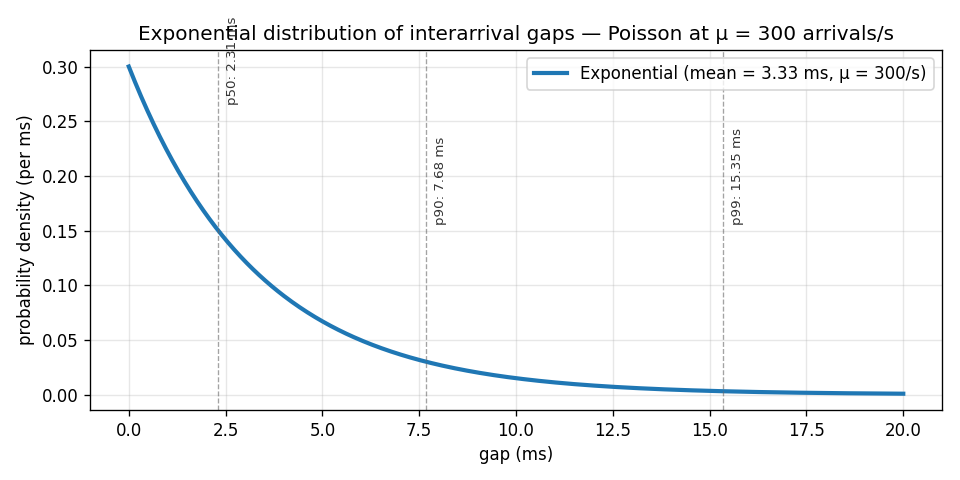
\includegraphics[width=0.7\textwidth]{figs/exponential_gaps.png}
  \caption{The exponential density of the gaps between arrivals of a Poisson process at $300$
  arrivals per second. Dashed vertical lines mark the median, the 90th and the 99th percentile.
  Half the gaps are shorter than the median of $2.3$\,ms and $10\%$ are longer than $7.7$\,ms. Real
  market-data streams have far more mass near zero and a much heavier right tail. Reproduced from
  \citet{maciejewski2026packets}.}
  \label{fig:exp-gaps}
\end{figure}

\paragraph{(2) The count in any window of length $w$ is Poisson-distributed.} Let $N_w$ be the
number of arrivals in a window of length $w$. Then
\[
  \E[N_w] = \mu w, \qquad \mathrm{Var}[N_w] = \mu w,
\]
so the ratio of variance to mean is $1$ for every $w$. This ratio is the \emph{Fano factor}
(Section~\ref{app:pp-fano}); a value other than $1$ rejects the Poisson model.

\paragraph{(3) Counts in non-overlapping windows are independent.} The number of arrivals in the
first second says nothing about the number in the next.

\paragraph{Poisson as the null hypothesis.} The Poisson process is the stream with no memory, no
clustering and no regularity: arrivals are as uncoordinated as possible. Any departure from it is
structure in the arrival stream.

\paragraph{Two ways a real feed departs from Poisson.} The first is \emph{bunching}: many gaps are
far shorter than the exponential law predicts ($73\%$ against $9.52\%$ above). The second is
\emph{memory in the rate}: after a burst starts, more arrivals are likely to follow. Modelling either
needs a process whose rate can change with its own history---a \emph{conditional-intensity point
process}.

\subsection{Points, processes and marks}
\label{app:pp-points}

\begin{itemize}[leftmargin=1.5em,itemsep=1pt]
\item A \textbf{point} is a single instant at which something happens, such as the timestamp of one
  packet or one order-book event.
\item A \textbf{process} is a random object that unfolds in time; here, a random list of arrival
  times $t_1 < t_2 < t_3 < \cdots$.
\item A \textbf{point process} is a random sequence of points on the time axis, specified by
  \emph{when} events happen and nothing else.
\end{itemize}
If each event carries additional information (side, price, size, message type), the process is a
\textbf{marked point process}: the timestamps are the points and the extra information is the
\emph{mark}. Four order-book messages in the first second of a session might read
\begin{verbatim}
09:30:00.001234567   Add,    bid 21432.50, size 3
09:30:00.001234571   Add,    ask 21432.75, size 5
09:30:00.017891234   Cancel, order X, bid 21432.25
09:30:00.238491702   Trade,  ask 21432.75, size 2
\end{verbatim}
The point process is the four timestamps; message type, side, price and size are marks. The
multivariate Hawkes process of Section~\ref{sec:hawkes} is a marked point process whose mark is the
event type $i$.

\subsection{The probability space}
\label{app:pp-probspace}

An arrival stream is modelled as a \textbf{stochastic process}, a family of random variables indexed
by time, on a probability space $(\Omega, \mathcal{A}, \P)$:
\begin{itemize}[leftmargin=1.5em,itemsep=1pt]
\item $\Omega$, the \emph{sample space}, is the set of all possible outcomes; here an outcome is one
  complete realisation of a session's arrivals.
\item $\mathcal{A}$, the \emph{$\sigma$-algebra}, is the collection of yes-or-no questions about the
  outcome to which a probability can be assigned, such as ``did at least one packet arrive between
  09:30:00 and 09:30:01?''. It is closed under negation and countable union.
\item $\P : \mathcal{A} \to [0, 1]$ assigns a probability to each such event, with
  $\P(\emptyset) = 0$, $\P(\Omega) = 1$, and probabilities of disjoint events adding up.
\end{itemize}

\subsection{History: information accumulated over time}
\label{app:pp-history}

The information available at time $t$ grows as time passes. Formally it is a
\textbf{filtration}, an increasing family of $\sigma$-algebras
\[
  \{\mathcal{I}_t\}_{t \ge 0}, \qquad \mathcal{I}_{t'} \subseteq \mathcal{I}_t \text{ for } t' \le t.
\]
$\mathcal{I}_t$ is everything observable up to and including time $t$, and $\mathcal{I}_{t-}$
everything observable strictly before $t$. ``Conditional on $\mathcal{I}_{t-}$'' means ``given
everything seen strictly before $t$''. In the main text this is what conditioning on $X_t$ means: a
model may use only what is in the history.

\subsection{The counting process}
\label{app:pp-counting}

The observable object is the random step function
\[
  N(t) = \#\{\, n : t_n \le t \,\},
\]
the number of arrivals up to time $t$. It starts at $N(0) = 0$, never decreases, and jumps by one at
each arrival. The number of arrivals in the interval $(t, t + \Delta t]$ is $N(t + \Delta t) - N(t)$.

\subsection{Conditional intensity}
\label{app:pp-intensity}

At time $t$, ask for the probability that at least one arrival occurs in the next short interval of
length $\Delta t$, given everything seen so far. The \textbf{conditional intensity} is that
probability divided by $\Delta t$, in the limit of a very short interval:
\[
  \lambda(t \mid \mathcal{I}_{t-}) = \lim_{\Delta t \downarrow 0} \frac{1}{\Delta t}\;
  \P\big( N(t + \Delta t) - N(t) \ge 1 \,\big|\, \mathcal{I}_{t-} \big).
\]
It is the instantaneous arrival rate given the history, in arrivals per second; in the rest of the
paper it is written simply $\lambda(t)$. At an intensity of $300$ per second the probability of an
arrival in the next millisecond is about $\lambda(t)\,\Delta t = 300 \times 0.001 = 0.3$. For a short
interval, and for the expected count over a longer one,
\[
  \P\big(\text{arrival in } (t, t+\Delta t]\big) \approx \lambda(t)\, \Delta t, \qquad
  \E\big[N(t+w) - N(t)\big] = \E\!\int_{t}^{t+w} \lambda(t')\, dt'.
\]
Specifying $\lambda$ as a function of the history specifies the point process completely. For a
Poisson process $\lambda(t) = \mu$ and the history carries no information. For a Hawkes process the
intensity is $\mu$ plus a decaying contribution from each past arrival.

\subsection{Three canonical models: Poisson, renewal and Hawkes}
\label{app:pp-canon}

\paragraph{(a) Poisson.} $\lambda(t) = \mu > 0$. Gaps are independent and exponential with mean
$1/\mu$; the count in a window of length $w$ is Poisson with mean $\mu w$. Every summary statistic
takes its reference value: the Fano factor is $1$ at every $w$, the Hurst exponent is $0.5$, and the
gaps are uncorrelated.

\paragraph{(b) Renewal process.} The gaps $\Delta t_n = t_n - t_{n-1}$ are independent draws from a common
distribution, not necessarily exponential. The intensity depends only on the time since the last
arrival. A renewal process is Poisson only when the gaps are exponential. Heavy-tailed gaps produce
many short gaps and a Fano factor well above $1$, but the Fano factor levels off as $w$ grows instead
of continuing to rise, and the gaps are uncorrelated. Randomly shuffling the order of the gaps leaves
a renewal process statistically unchanged; comparing a statistic on a real stream with the same
statistic on its shuffled gaps therefore separates what the \emph{order} of the gaps carries from
what their \emph{lengths} carry.

\paragraph{(c) Hawkes (self-exciting) process.} Each past arrival raises the intensity for a while:
\[
  \lambda(t) = \mu + \sum_{n:\, t_n < t} \phi(t - t_n).
\]
$\mu \ge 0$ is the \textbf{background rate}, the intensity with no prior arrivals.
$\phi$ is the \textbf{kernel}: an arrival $u$ seconds ago still contributes $\phi(u)$ to the
intensity now. The kernel is the shape of one event's influence on the future. Dropping several
stones into a pond is the usual picture: the disturbance at any moment is the sum of the ripples
still spreading, each faded by the time since its stone fell. For the self-exciting specification
used here the kernel is non-negative, so a past event can only raise future intensity (inhibitory
extensions are discussed in Section~\ref{sec:hawkes-variants}), and its total area
must be finite, so that the past does not accumulate without bound. This is the one-type case of
the multivariate model in Section~\ref{sec:hawkes}.

\paragraph{Kernel families.} The \emph{exponential kernel} $\phi(u) = \alpha\, \mathrm{e}^{-\omega u}$ has
two parameters: $\alpha \ge 0$, the jump in intensity immediately after an arrival, and
$\omega > 0$, the decay rate, whose inverse $1/\omega$ is the kernel's decay time. It is Markovian:
the current intensity summarises everything needed from the past. Right after an arrival the
intensity rises by $\alpha$; between arrivals it relaxes toward $\mu$ as
$\mu + (\lambda(t_n) - \mu)\, \mathrm{e}^{-\omega u}$; so it can be updated in constant time per arrival---a useful
property for a low-latency system. The \emph{power-law kernel} $\phi(u) = \alpha\,(1 + u/u_0)^{-(1+\zeta)}$, with
the same jump $\alpha$, a time scale $u_0 > 0$ and an exponent $\zeta > 0$, decays more slowly; \citet{hardimanbercotbouchaud2013} find power-law kernels on
E-mini S\&P mid-price changes over lags from seconds to days.

\subsection{Branching ratio}
\label{app:pp-branching}

\[
  \Gamma = \int_0^\infty \phi(u)\, du, \qquad \Gamma = \alpha/\omega \text{ for the exponential kernel}.
\]
$\Gamma$ is the mean number of arrivals that one arrival triggers \emph{directly}. The Hawkes process
is equivalently a \textbf{branching process}~\citep{hawkesoakes1974}: every arrival is either an
\emph{immigrant}, generated by the background rate $\mu$, or the \emph{child} of an earlier arrival,
and each arrival has on average $\Gamma$ children. The expected size of the family descended from one
immigrant is the geometric series
\[
  1 + \Gamma + \Gamma^2 + \Gamma^3 + \cdots = \frac{1}{1 - \Gamma} \qquad (\Gamma < 1),
\]
which is the one-type case of the series for $(I - \Gamma)^{-1}$ in Section~\ref{sec:hawkes}. For
$\Gamma < 1$ the process is \emph{subcritical}: families are finite and the long-run rate is
$\bar\lambda = \mu / (1 - \Gamma)$. As $\Gamma \to 1$ it becomes \emph{near-critical}: family sizes
and durations grow without bound and long-range dependence appears. At $\Gamma = 1$ the process is
\emph{critical}: each family still dies out with probability one, but its expected size is infinite,
and with a positive background rate there is no stationary version. For $\Gamma > 1$ it is
\emph{supercritical}: with positive probability one arrival starts a cascade that never ends, and the
intensity grows without bound.

On CME NQ market data, an exponential-kernel fit gives $\Gamma \approx 0.80$ on both packets and
matching-engine transactions, with a kernel decay time $1/\omega$ of about $167\,\mu$s: four of every
five arrivals are triggered by earlier ones~\citep{maciejewski2026packets}.
On E-mini S\&P futures, \citet{filimonovsornette2012} report $0.7$--$0.8$ after 2007, with spikes
to $0.9$, and \citet{hardimanbercotbouchaud2013} report values near $1$ for mid-price changes; \citet{filimonovsornette2015} show that a fit with a
constant background rate, over a window in which the true background varies, overstates $\Gamma$.

\paragraph{The critical boundary in practice.} At $\Gamma = 1$ the stationary rate
$\mu/(1-\Gamma)$ is infinite. On a finite window the process still fires finitely often, but the
variance of the count grows faster than linearly with the window. A maximum-likelihood fit that
lands at $\Gamma = 1$ on real data may signal non-stationarity, a mis-specified kernel or a numerical
problem rather than a genuinely critical market; whether markets are critical or merely close to it is
itself debated~\citep{hardimanbercotbouchaud2013,filimonovsornette2015}.

\subsection{What Hawkes processes look like}
\label{app:pp-visualise}

The long-run rate $\bar\lambda = \mu/(1-\Gamma)$ and the branching ratio $\Gamma$ look different in
an event raster. Figure~\ref{fig:hawkes-grid} simulates an exponential-kernel Hawkes process over
15 seconds at nine combinations, $\bar\lambda \in \{2, 10, 50\}$ events per second and
$\Gamma \in \{0.30, 0.60, 0.90\}$, with a kernel decay time of one second. At low rate and low
branching ratio the stream is nearly Poisson: arrivals spread evenly, the count grows in a straight
line, the intensity is flat. At high rate and low branching ratio it is dense but still nearly
Poisson. At low rate and high branching ratio the mean is 2 per second but arrivals come in
unmistakable bursts, with long empty stretches between them and the intensity reaching 20--30 per
second inside a burst. At high rate and high branching ratio the intensity swings by an order of
magnitude within the window.

\begin{figure}[ht]
  \centering
  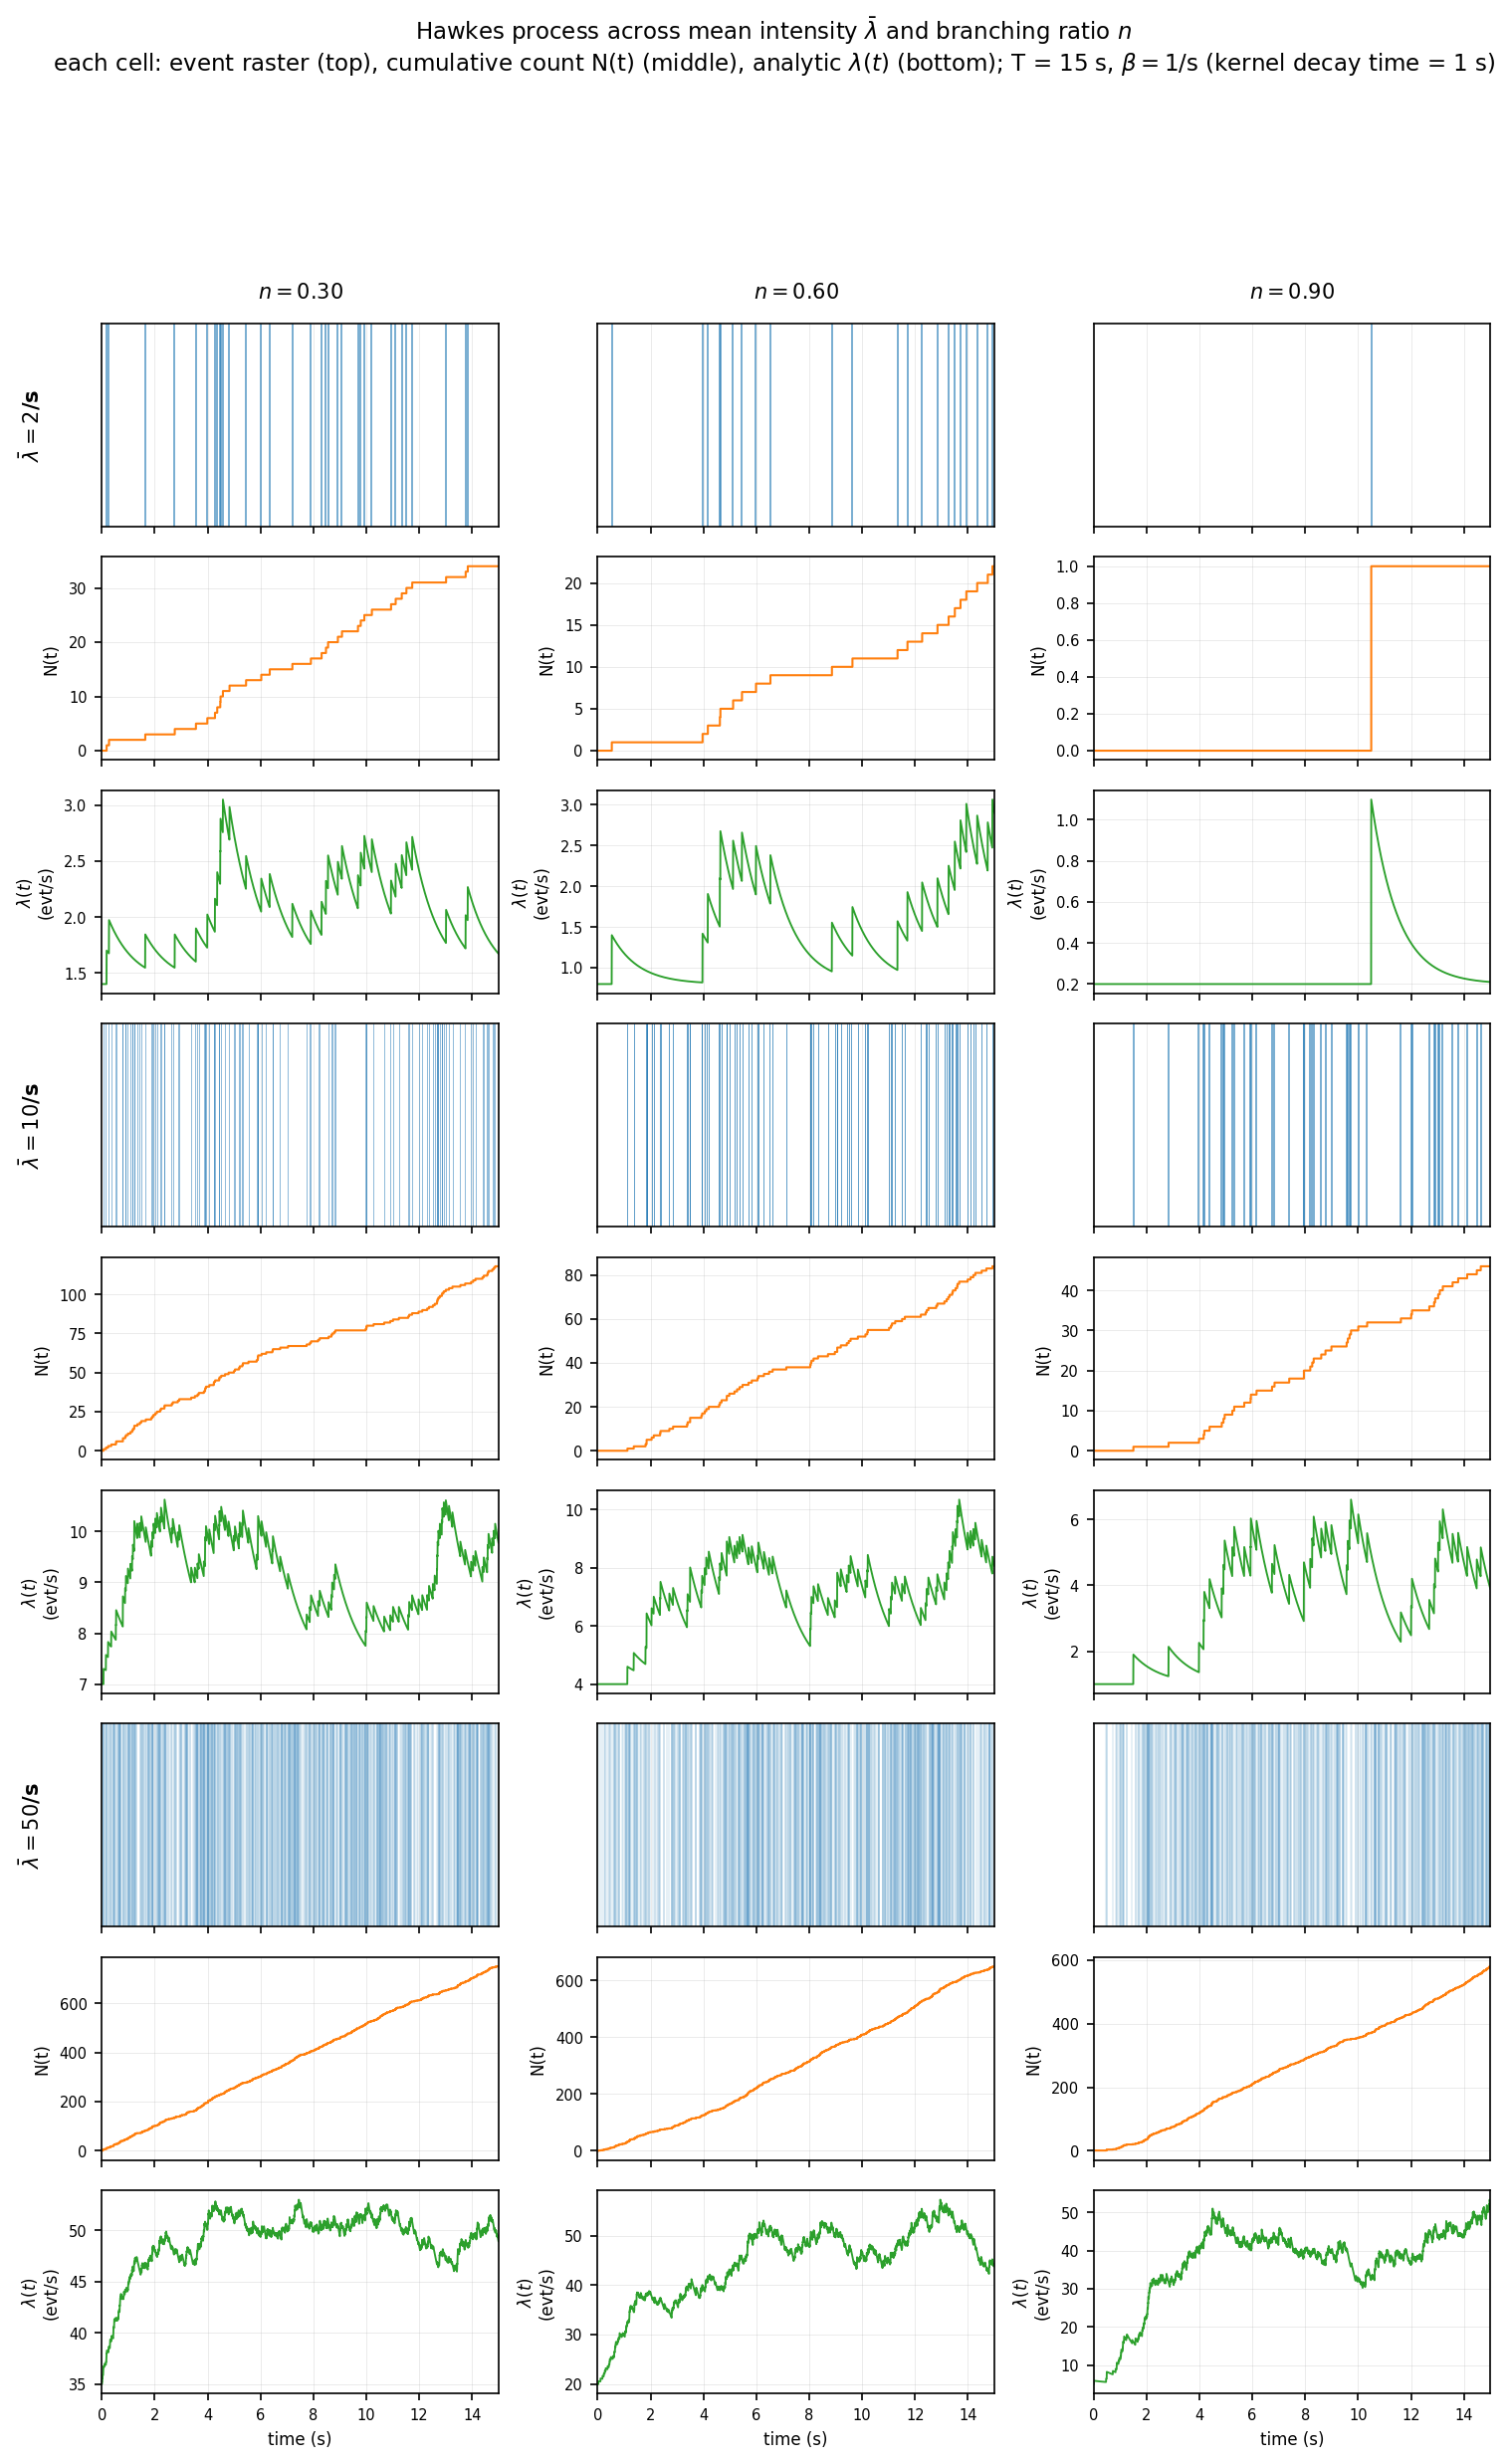
\includegraphics[width=\textwidth,height=0.82\textheight,keepaspectratio]{figs/hawkes_grid_3x3.png}
  \caption{Simulated exponential-kernel Hawkes processes. Each cell stacks the event raster (top),
  the cumulative count $N(t)$ (middle) and the intensity $\lambda(t)$ (bottom). Rows: long-run rate
  $\bar\lambda \in \{2, 10, 50\}$ events per second. Columns: branching ratio
  $\Gamma \in \{0.30, 0.60, 0.90\}$. Fifteen seconds, decay rate $\omega = 1/\mathrm{s}$. The time
  scale is chosen for legibility; the kernel fitted on CME data decays about four orders of
  magnitude faster. Reproduced from \citet{maciejewski2026packets}. Labels inside the image use the source's notation: $n$ for $\Gamma$, $\beta$ for $\omega$, $F$ for $D$ and $\tau$ for $w$.}
  \label{fig:hawkes-grid}
\end{figure}

\subsection{Three signatures that separate Poisson, renewal and Hawkes processes}
\label{app:pp-signatures}

\emph{(i) An excess of short gaps.} On CME NQ packet data $73\%$ of gaps are shorter than a tenth of
the mean gap; any exponential gives $9.52\%$. A Hawkes process produces such an excess, but so does a
renewal process with heavy-tailed gaps, so this signature rejects Poisson without identifying
self-excitation.

\emph{(ii) Correlated gaps.} Under self-excitation, short gaps tend to follow short gaps and long
gaps follow long ones, so successive gaps are positively correlated. A renewal process has
independent gaps. A rate that varies slowly over the observation window also produces positive gap
correlation, so this signature has to be checked against that alternative.

\emph{(iii) Burstiness that grows with the time scale.} The Fano factor rises with the window length
on a Hawkes process and levels off on a Poisson or renewal process. Clustering is then not a feature
of one time scale but looks similar over decades of window lengths. A slowly varying rate can also
make the Fano factor rise, which is the effect \citet{filimonovsornette2015} warn about.

\subsection{Fano factor}
\label{app:pp-fano}

For a window length $w$, cut the observation period into $\Upsilon$ consecutive windows and let
$N_{w,\upsilon} = N(\upsilon w) - N((\upsilon-1)w)$ be the count in window $\upsilon$. The Fano factor, also called the
\emph{index of dispersion}, is
\[
  D(w) = \frac{\mathrm{Var}[N_{w,\upsilon}]}{\E[N_{w,\upsilon}]},
\]
the variance of the window counts divided by their mean. For a Poisson process $D(w) = 1$ at every
$w$. For a renewal process with finite-variance gaps $D(w)$ tends to a constant as $w$ grows. For a
clustered process $D(w) > 1$, and under self-excitation or a varying rate it keeps growing with $w$.
The measure is named after U.~Fano, who introduced it for fluctuations in counts of ions. On CME NQ
packet data $D(w)$ grows from about $52$ at $w = 0.1$\,s to about a thousand at $w = 60$\,s, while
the same stream with its gaps shuffled stays flat at about $17$~\citep{maciejewski2026packets}.

\begin{figure}[ht]
  \centering
  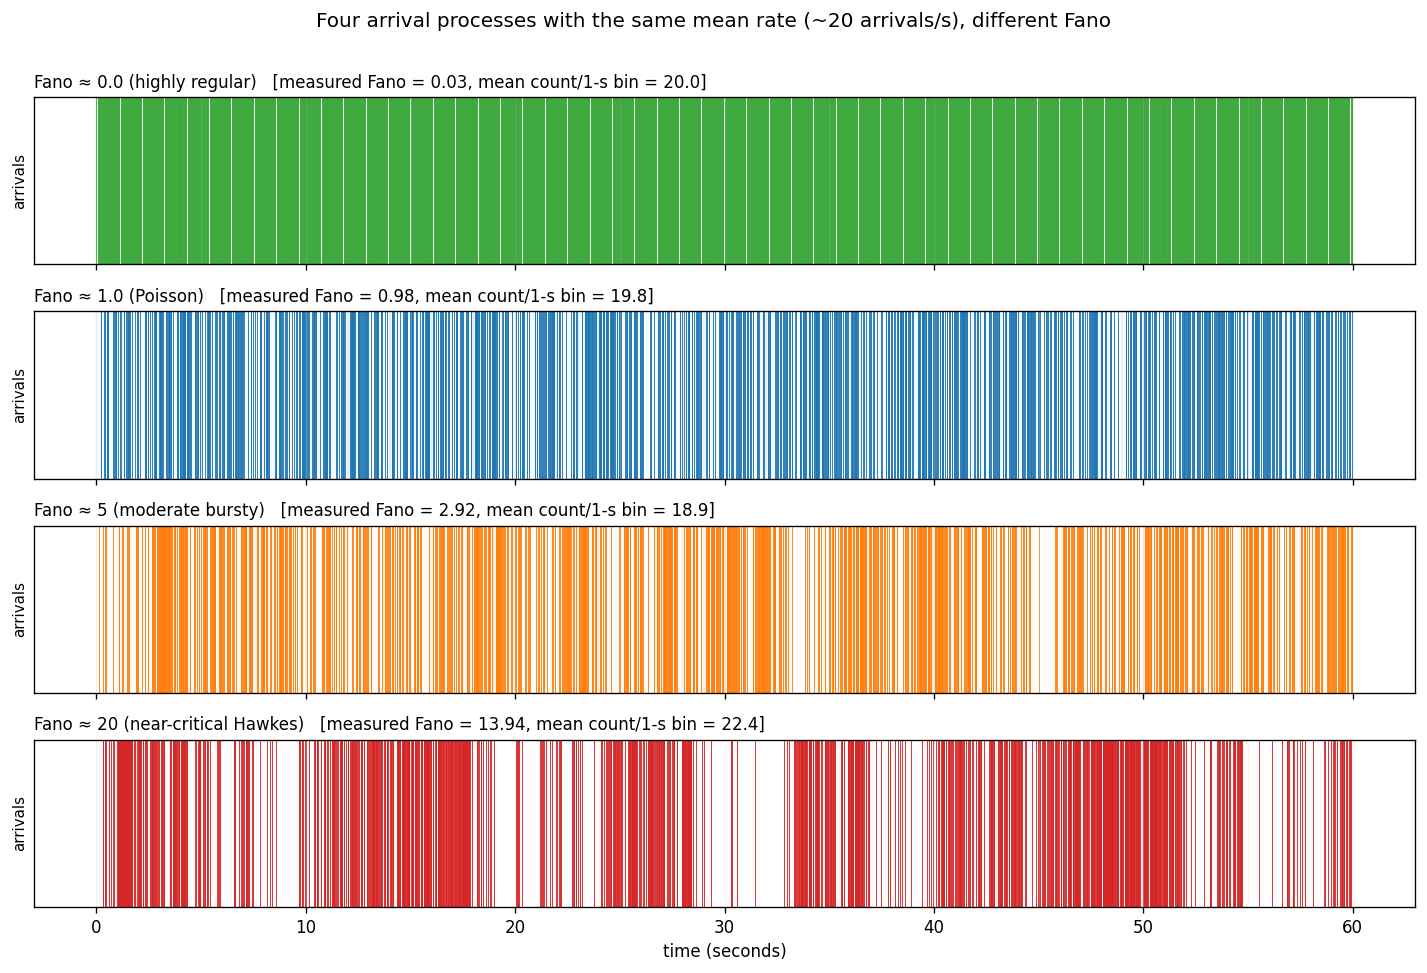
\includegraphics[width=\textwidth]{figs/rasters_by_fano.png}
  \caption{Four simulated processes at the same mean rate of about 20 per second. Top row
  ($D \approx 0$, highly regular): near-lattice arrivals, nearly equal counts per window. Second row
  ($D \approx 1$, Poisson): the reference. Third row ($D \approx 3$, moderate Hawkes): visible
  clumping. Bottom row ($D \approx 14$, near-critical Hawkes): pronounced bursts and long quiet
  stretches, with window counts from near zero to over 50. Reproduced from
  \citet{maciejewski2026packets}. Labels inside the image use the source's notation: $n$ for $\Gamma$, $\beta$ for $\omega$, $F$ for $D$ and $\tau$ for $w$.}
  \label{fig:rasters-fano}
\end{figure}

\begin{figure}[ht]
  \centering
  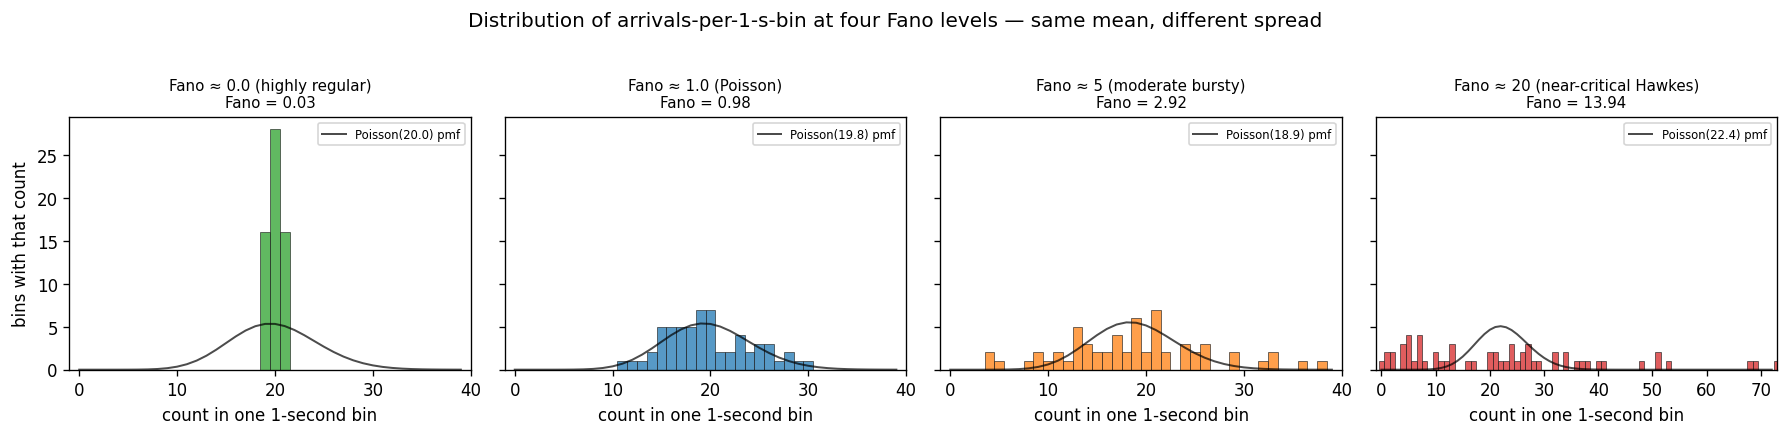
\includegraphics[width=\textwidth]{figs/count_hists_by_fano.png}
  \caption{Distribution of arrivals per one-second window (bars) for the four processes of
  Figure~\ref{fig:rasters-fano}, with the Poisson distribution of the same mean overlaid (curve).
  $D \approx 0$: narrower than Poisson. $D \approx 1$: matches Poisson. $D > 1$: wider than Poisson,
  with extra mass in both tails. The CME NQ packet stream has $D(1\,\mathrm{s}) = 108$, far wider
  than any panel shown. Reproduced from \citet{maciejewski2026packets}. Labels inside the image use the source's notation: $n$ for $\Gamma$, $\beta$ for $\omega$, $F$ for $D$ and $\tau$ for $w$.}
  \label{fig:counthist-fano}
\end{figure}

\subsection{Hurst exponent from the scaling of the Fano factor}
\label{app:pp-hurst}

When the Fano factor grows as a power of the window length,
\[
  D(w) \propto w^{2\mathcal{H} - 1},
\]
the exponent $\mathcal{H}$ is the \emph{Hurst exponent}. $\mathcal{H} = 0.5$ means no long-range
dependence (Poisson, and renewal processes with finite-variance gaps); $0.5 < \mathcal{H} < 1$ means
long-range dependence, with clustering that looks similar across time scales; $\mathcal{H}$ near $1$
means very long memory. It is estimated by a straight-line fit on a log--log plot,
\[
  \ln D(w) = (2\mathcal{H} - 1)\ln w + \text{constant},
\]
so $\mathcal{H} = (\text{slope} + 1)/2$. On CME NQ packet data $\mathcal{H} \approx 0.74$; shuffling
the gaps, which keeps their lengths and destroys their order, takes it to $0.50$, so the long-range
dependence lives in the order of the gaps~\citep{maciejewski2026packets}.

\begin{figure}[ht]
  \centering
  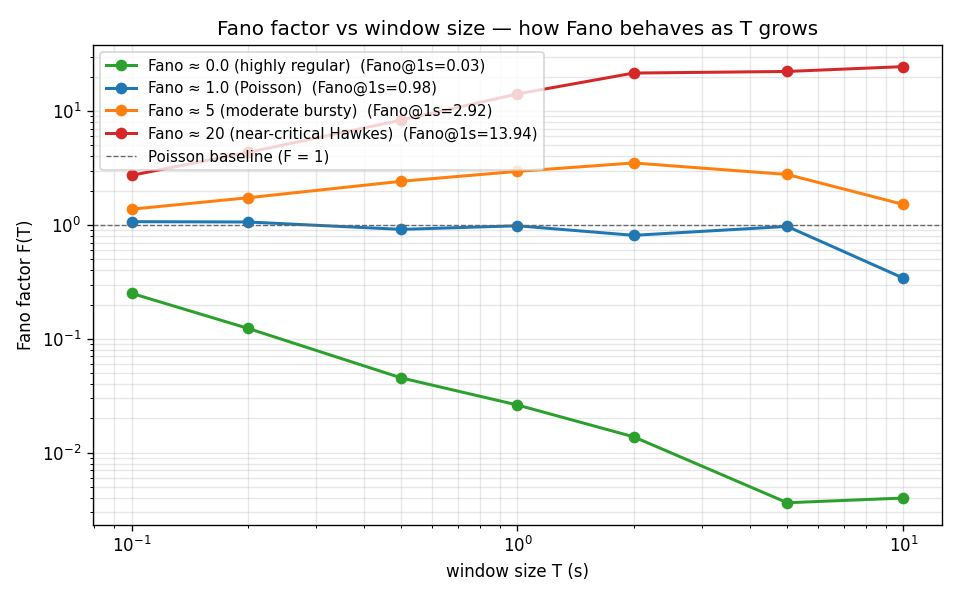
\includegraphics[width=0.7\textwidth]{figs/fano_scaling.png}
  \caption{The Fano factor $D(w)$ against the window length $w$ on logarithmic axes for four
  simulated processes. Regular: near zero. Poisson: flat at 1. Moderate Hawkes: rising. Near-critical
  Hawkes: a steeper rise, with slope about $0.5$, i.e.\ $\mathcal{H} \approx 0.75$. Reproduced from
  \citet{maciejewski2026packets}. Labels inside the image use the source's notation: $n$ for $\Gamma$, $\beta$ for $\omega$, $F$ for $D$ and $\tau$ for $w$.}
  \label{fig:fano-scaling}
\end{figure}

\subsection{Fitting an exponential-kernel Hawkes process}
\label{app:pp-mle}

The input is a sorted list of arrival times $t_1 < \cdots < t_{N_{\text{end}}}$ in a window
$[0, t_{\text{end}}]$, where $N_{\text{end}} = N(t_{\text{end}})$ is the number of arrivals, and
there are three parameters:
\begin{itemize}[leftmargin=1.5em,itemsep=1pt]
\item $\mu$, the \textbf{background rate}: arrivals per second with no recent history;
\item $\alpha$, the \textbf{jump}: the rise in intensity, in arrivals per second, at each arrival;
\item $\omega$, the \textbf{decay rate}: each jump fades as $\mathrm{e}^{-\omega u}$, with decay time
  $1/\omega$.
\end{itemize}
Fitting means choosing the parameters under which the observed timestamps are most probable, that
is, maximising the log-likelihood~\citep{ozaki1979}
\begin{equation}
  \ln \mathrm{Lik}(\mu, \alpha, \omega) = \sum_{n=1}^{N_{\text{end}}} \ln \lambda(t_n)
  - \int_0^{t_{\text{end}}} \lambda(t')\, dt'.
  \label{eq:hawkes-loglik}
\end{equation}
\inwords{the first term rewards the model for predicting a high rate at the moments arrivals
actually happened; the second penalises it for predicting more arrivals in total than occurred. If
$\alpha$ is too small the model cannot explain the bursts; if $\alpha$ approaches $\omega$ it predicts
more clustering than there is; a wrong $\mu$ misexplains the quiet periods.}

For the exponential kernel both terms can be computed in one pass over the data. With
\[
  \Psi_n = \mathrm{e}^{-\omega (t_n - t_{n-1})}\,(1 + \Psi_{n-1}), \qquad \Psi_1 = 0,
\]
the intensity at each arrival is $\lambda(t_n) = \mu + \alpha \Psi_n$, and the integral is
\[
  \int_0^{t_{\text{end}}} \lambda(t')\, dt' = \mu\, t_{\text{end}}
  + \frac{\alpha}{\omega} \sum_{n=1}^{N_{\text{end}}} \Big(1 - \mathrm{e}^{-\omega (t_{\text{end}} - t_n)}\Big).
\]
Timestamps are shifted to the start of the window before fitting, so that the exponentials do not
underflow. The log-likelihood is then maximised numerically over $(\mu, \alpha, \omega)$, for example
with the Nelder--Mead method, and the optimum checked with a second optimiser. From the fitted
parameters follow the branching ratio $\Gamma = \alpha/\omega$, the kernel decay time $1/\omega$, and
the long-run rate $\bar\lambda = \mu/(1 - \Gamma)$: the background rate amplified by $1/(1-\Gamma)$
through self-excitation.

\subsection{Symbols used in this appendix}

\begin{center}\small
\begin{tabular}{@{}ll@{}}
\toprule
Symbol & Meaning \\
\midrule
$\Omega$, $\mathcal{A}$, $\P$ & sample space, $\sigma$-algebra, probability \\
$\mathcal{I}_t$, $\mathcal{I}_{t-}$ & everything observable up to $t$ inclusive / strictly before $t$ \\
$t_1, t_2, \ldots$ & arrival times \\
$N(t)$ & counting process, the number of arrivals up to $t$ \\
$\lambda(t)$ & conditional intensity, arrivals per second \\
$\mu$ & background rate \\
$\phi(u)$ & Hawkes kernel \\
$\alpha$, $\omega$ & exponential-kernel jump and decay rate; decay time $1/\omega$ \\
$\Gamma$ & branching ratio, $\int\phi$; $\alpha/\omega$ for the exponential kernel \\
$\bar\lambda = \mu/(1-\Gamma)$ & long-run mean rate \\
$\Delta t_n = t_n - t_{n-1}$ & gap between arrivals \\
$w$ & window length for counts \\
$N_{w,\upsilon}$, $\Upsilon$ & arrivals in window $\upsilon$; number of windows \\
$D(w)$ & Fano factor, variance over mean of the window counts \\
$\mathcal{H}$ & Hurst exponent, $D(w) \propto w^{2\mathcal{H}-1}$ \\
$\Psi_n$ & running sum used to compute $\lambda(t_n)$ in one pass \\
\bottomrule
\end{tabular}
\end{center}


\FloatBarrier
\bibliographystyle{plainnat}
\bibliography{refs,bib/refs_classic,bib/refs_dl,bib/refs_eval,bib/refs_fm,bib/refs_hawkes2}

\end{document}
